\documentclass[11pt,letterpaper]{article}
\usepackage[T1]{fontenc}
\usepackage{lmodern}
\usepackage[letterpaper,textwidth=449pt,textheight=650pt,hcentering,top=73pt,headheight=14pt,headsep=18pt]{geometry}
\usepackage{amsthm,mathtools,amssymb,microtype}
\usepackage{graphicx,tikz,booktabs,enumitem,fancyhdr}
\usetikzlibrary{arrows.meta,calc,positioning}
\usepackage[font=small,labelfont=bf,labelsep=period]{caption}
\definecolor{ink}{HTML}{213650}
\definecolor{lagoon}{HTML}{175967}
\definecolor{ember}{HTML}{994121}
\usepackage[unicode,colorlinks,linkcolor=ink,citecolor=lagoon,urlcolor=lagoon,
 pdfauthor={OpenAI},pdftitle={Superpolynomial graph diameter of simple polytopes},
 pdfsubject={Superpolynomial-graph-diameter-of-simple-polytopes-November-24-2026}]{hyperref}
\usepackage{bookmark}
\input glyphtounicode
\pdfgentounicode=1
\setcounter{tocdepth}{1}
\pagestyle{fancy}
\fancyhf{}
\fancyhead[L]{\small\color{black!65}\nouppercase{\leftmark}}
\fancyhead[R]{\small\thepage}
\renewcommand{\sectionmark}[1]{\markboth{\thesection.\ #1}{}}
\renewcommand{\headrulewidth}{0pt}
\setlist[itemize,enumerate]{topsep=4pt plus 1pt,itemsep=2pt,parsep=0pt}
\linespread{1.025}
\raggedbottom
\emergencystretch=1.0em
\widowpenalty=6000
\clubpenalty=3500
\newtheorem{theorem}{Theorem}[section]
\newtheorem{lemma}[theorem]{Lemma}
\newtheorem{proposition}[theorem]{Proposition}
\newtheorem{corollary}[theorem]{Corollary}
\theoremstyle{definition}
\newtheorem{definition}[theorem]{Definition}
\newtheorem{example}[theorem]{Example}
\theoremstyle{remark}
\newtheorem{remark}[theorem]{Remark}

\title{Superpolynomial graph diameter\\of simple polytopes}
\author{OpenAI}
\date{November 24, 2026}
\makeatletter
\renewcommand{\maketitle}{%
  \begin{center}
    {\fontsize{21}{25}\selectfont\bfseries\color{ink}\@title\par}\vspace{6pt}
    {\normalfont\large\@author\par}\vspace{2pt}
    {\normalfont\normalsize\@date\par}
  \end{center}\thispagestyle{plain}}
\renewcommand*{\l@section}{\@dottedtocline{1}{0em}{2.05em}}
\makeatother

\begin{document}
\maketitle
\begin{abstract}
\normalsize\noindent
We disprove the polynomial Hirsch conjecture. For every sufficiently large
\(n\), we construct a bounded simple rational polytope with exactly \(n\)
facets whose graph diameter grows faster than every fixed power of \(n\).
Its dimension grows more slowly than every positive power of \(n\).
For any prescribed subpolynomial \(s(n)\), two vertices can remain
superpolynomially far apart even when a single step may cross any face
of dimension at most \(s(n)\).
\end{abstract}
\section{Introduction}\label{sec:introduction}

How many edges must one traverse to get from one vertex of a polytope to
another? In 1957 Hirsch proposed that a \(d\)-dimensional polyhedron with
\(n\) facets should require at most \(n-d\) steps. Santos disproved this
bound for bounded polytopes by constructing an example of dimension \(43\)
with \(86\) facets and two vertices at least \(44\) steps apart~\cite{santos}.
That example left open the possibility that some polynomial in \(n\)
bounds all such distances. We construct bounded polytopes whose diameter
grows faster than every fixed power of their facet count.

The diameter is the maximum, over all pairs of vertices, of the length of
a shortest path in the undirected vertex--edge graph. Our examples are
\emph{simple}, meaning that every vertex lies on exactly \(d\) facets.
We can even allow a move directly between any two vertices of a common
face of dimension at most \(s\). Write \(\operatorname{dist}_s(v,w)\)
for the minimum number of these moves, so that \(\operatorname{dist}_1\)
is the usual graph distance. For a positive function of \(n\), the
notations \(n^{o(1)}\) and \(n^{\omega(1)}\) mean that the ratio of
its logarithm to \(\log n\) tends to zero and to infinity, respectively.

\begin{theorem}[Superpolynomial diameter]\label{thm:main}
For each positive integer-valued \(s(n)=n^{o(1)}\) there is a family
of bounded simple rational polytopes \(P_n\), one for every sufficiently
large \(n\), with exactly \(n\) facets, dimension \(n^{o(1)}\), and
\(s(n)\)-move diameter \(n^{\omega(1)}\).

Moreover, there is a linear functional \(x\) on each \(P_n\), of positive
range \(\Delta x=\max_{P_n}x-\min_{P_n}x\), such that for every fixed
\(0<\alpha<1\),
\[
 \min_{\substack{v,w\ \mathrm{vertices\ of}\ P_n\\
               |x(v)-x(w)|\ge n^{-\alpha}\Delta x}}
       \operatorname{dist}_{s(n)}(v,w)=n^{\omega(1)}.
\]
\end{theorem}

Taking \(s(n)=1\) disproves the polynomial Hirsch conjecture. The objective
estimate explains where the long distances occur. On the same polytope,
every pair of vertices separated by even a fraction \(n^{-\alpha}\) of
the objective range requires a long walk. Intermediate vertices may take
any objective values.

There is also a bound with both the dimension \(d\) and the facet excess
\(E=n-d\) prescribed. This includes the classical \(d\)-step case
\(E=d\), as well as regimes in which the two parameters grow at very
different rates.

\begin{theorem}[Prescribed dimension and facet excess]\label{thm:excess}
For any \(a,b>0\) there exist \(c,\delta>0\) such that, for all
integers \(d,E\) with \(m=\min\{d,E\}\) sufficiently large, some
rational simple \(d\)-polytope with exactly \(d+E\) facets has two
vertices requiring at least
\[
                         cE\min\{E^a,d^b\}
\]
moves across faces of dimension at most \(\lfloor m^\delta\rfloor\).
\end{theorem}

At \(n=2d\), for every prescribed \(s(d)=d^{o(1)}\), there are
vertices at \(s(d)\)-move distance \(d^{\omega(1)}\) such that each
facet contains exactly one of them (Corollary~\ref{cor:spindle}).
In the polar these vertices correspond to two disjoint simplex facets
that together contain every vertex. A section between the facets yields
a Minkowski sum of two simplices with superpolynomial facet-adjacency
diameter (Corollary~\ref{cor:minkowski}).

\subsection{Diameter and linear programming}

The simplex method gives Hirsch's question an algorithmic interpretation.
Starting from a feasible vertex, a pivot can move to an adjacent vertex.
Even complete knowledge of the destination cannot shorten a walk below
the graph distance. General LP algorithms have other choices.
In the companion paper~\cite{lpcompanion}, a strongly polynomial algorithm
finds an optimum by recovering its primal and dual certificates from the
inequalities. Corollary~\ref{cor:packing} makes this distinction concrete. It gives
packing linear programs in which the origin and the all-ones vector are
the unique minimizer and maximizer of the sum of the coordinates, yet
every edge path between these explicit endpoints has superpolynomial length.

Dantzig recorded Hirsch's original question in his treatment of linear
programming~\cite[p.~160]{dantzig}. Klee and Walkup reduced the linear
conjecture to the case \(n=2d\) and gave an unbounded counterexample~\cite{kw}.
For bounded polytopes, Matschke, Santos and Weibel brought the dimension
of Santos's counterexample down to \(20\)~\cite{msw}. Davies and
coauthors constructed five-dimensional prismatoids whose width grows
linearly in their number of vertices~\cite{davies}. The polynomial
conjecture asks for a single polynomial valid in all dimensions
\cite[Conjecture~1.3]{santos}.

Larman's upper bound \(n\,2^{O(d)}\) shows that a superpolynomial
diameter forces \(d/\log n\) to tend to infinity~\cite{larman}.
Theorem~\ref{thm:main} places the examples within this range while
keeping \(d\) smaller than every positive power of \(n\).
The Kalai--Kleitman bound and its refinements give quasipolynomial upper
bounds as \(d\) varies~\cite{kalai,todd,sukegawa}. Liu, Ge and Ye
also obtain a quasipolynomial upper bound in the facet excess alone
\cite{liugeye}. Our construction concerns actual convex polytopes.
It complements work on combinatorial models of diameter, including
connected layer families~\cite{abstraction}. By polarity, the examples
also give rational simplicial polytopes whose facets have superpolynomial
diameter under adjacency across ridges~\cite{ziegler}.

\subsection{Why distances multiply}

The construction uses a linear coordinate \(x\) to measure progress through
a polyhedron. We call \(x\) \emph{time}, although a path can move in either
direction in \(x\). The elementary way to force a bend is to give
\(J+1\) independent coordinates \(z_i\) the lower bounds
\(z_i\ge |x-a|\). At a fixed \(x\), a point in a face of the slice of
dimension at most \(J\) must attain at least one bound. In particular,
some \(z_i=0\) when the path reaches \(x=a\). If an affine segment
crossed that level in its interior, its \(z_i\) coordinate would give a
line through the corner lying above both branches of \(|x-a|\).
Figure~\ref{fig:kink} shows why this is impossible. A convex piecewise
affine lower bound with many corners forces a separate bend at each one.

\begin{figure}[htbp]
\centering
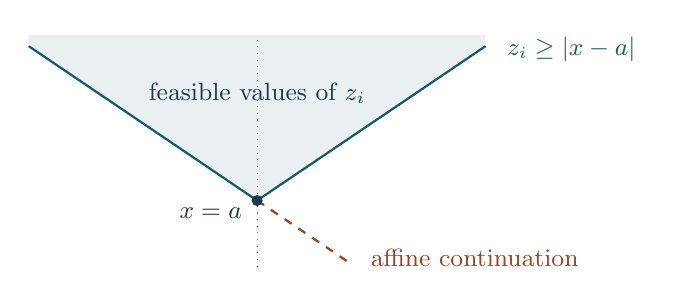
\begin{tikzpicture}[x=1cm,y=.8cm,font=\small,>=Stealth]
  \fill[lagoon!9] (-2.9,2.63) -- (-2.9,2.45) -- (0,0)
       -- (2.9,2.45) -- (2.9,2.63) -- cycle;
  \draw[lagoon,thick] (-2.9,2.45) -- (0,0) -- (2.9,2.45);
  \draw[ink!65,dotted] (0,-1.05) -- (0,2.64);
  \draw[ember,thick,dashed] (0,0) -- (1.21,-1.02);
  \fill[ink] (0,0) circle[radius=2pt];
  \node[left=2pt,ink] at (0,-.2) {\(x=a\)};
  \node[ink] at (0,1.7) {feasible values of \(z_i\)};
  \node[lagoon,anchor=west] at (3.05,2.4) {\(z_i\ge |x-a|\)};
  \node[ember,anchor=west] at (1.32,-.91) {affine continuation};
\end{tikzpicture}
\caption{A coordinate that attains its lower bound at \(x=a\) cannot be affine
through the crossing. Continuing the left branch past \(a\) violates the
right-hand inequality. More generally, the two inequalities require an
affine line through the contact point to have slope at most \(-1\) on the
left and at least \(1\) on the right.}
\label{fig:kink}
\end{figure}


To make the cost grow faster than the number of inequalities, we place
a copy of an expensive crossing inside each of many disjoint intervals
of \(x\). Within one such interval, called an \emph{episode}, a pair
of auxiliary coordinates records progress by its difference \(w\).
A pair can be chosen for which \(w\) crosses from near zero to near one.
Several disjoint triples of smaller intervals are marked on the \(w\)-axis.
On a traversal of a triple, either part of the path describes an entire
inner crossing, with \(w\) as its time, or the path crosses an overlap
of two phases in \(x\). We put another copy of the test in each such
overlap. Figure~\ref{fig:episode} shows the two time coordinates.
The last overlaps in this recursion use the piecewise affine lower
bounds above.

The lower bound for the inner crossing is counted repeatedly. For a
sufficiently large crossing cost \(D\), one level with \(N\) episodes
and \(q\) triples per episode forces at least \(NqD/4\) segments. To count them
on an undirected walk, for each interval stop at the first hit of its
far endpoint and look back to the last hit of its near endpoint. The
selected subpaths occupy disjoint intervals of the \emph{path parameter}.
Even two visits to the same physical overlap can force different bends
(Figure~\ref{fig:return-traversals}).

The cost in facets is a separate matter. Giving every inner crossing
its own variables and inequalities would spend the very factor the
construction gained in distance. The copies instead use common clock
readings. Different copies on the same bank of clocks can contribute
tight inequalities only in disjoint reading intervals. Eliminating the
readings therefore requires combinations containing at most one row
from an inner copy. When a coordinate needed for that copy is missing,
a prescribed group of slacks can take its place. The scheduler is the
system of inequalities that makes the required slacks available at
the appropriate times. It must do this for many episodes using few
coordinates.

Section~\ref{sec:diameter} converts a finite crossing bound into
Theorems~\ref{thm:main} and~\ref{thm:excess}, including the passage
to bounded simple rational polytopes with an exact facet count.
Sections~\ref{sec:framework}--\ref{sec:recursion} establish the crossing
bound using the scheduler. Its numerical input is Theorem~\ref{thm:coarse},
which assigns states to successive times subject to a coordinatewise
inequality between neighbors. Sections~\ref{sec:numerical}--\ref{sec:finite}
construct these states and prove the inequality.
Sections~\ref{sec:layers}--\ref{sec:compiler} turn them into the scheduler's
linear constraints. Section~\ref{sec:geometry} gives the consequences
for complementary vertices, Minkowski sums and packing linear programs.

\clearpage
{\small\tableofcontents}
\medskip
\section{From crossings to diameter}\label{sec:diameter}

A move in a face can be drawn as a straight chord. We force a path of
such chords to change direction many times as it crosses the level
sets of a linear functional. The construction starts with a polyhedron
\(Q\) in coordinates \((x,z)\in\mathbb R\times\mathbb R^p\). We call
\(x\) the time and write \(Q(x)=\{z:(x,z)\in Q\}\). A \emph{crossing}
of a closed interval is a polygonal path in \(Q\) that joins its two
endpoint slices and stays between them. Its time coordinate may reverse
direction any number of times. A \emph{segmentation} partitions the
parameter interval into affine pieces. Its interior partition points
are the \emph{breaks}.

\begin{theorem}[Finite-scale crossing bound]\label{thm:seed}
Fix an integer \(K\ge2\) and \(0<\eta<1\). There are an integer
\(L\ge2\) and a constant \(\gamma>0\) with the following property. For
every sufficiently large power \(N=L^h\), every integer \(R\ge1\), and
every choice of \(N\) pairwise disjoint nondegenerate closed intervals in
\((0,1)\), there is a polyhedron \(Q\) defined by \(F\) inequalities of
the form \(c\cdot z\ge\ell(x)\), with \(c\ge0\) nonzero and \(\ell\)
affine. Each coordinate of \(z\) has an individual lower bound among
these rows, and
\[
                  p+1\le N^\eta,\qquad F+3\le R N^{1+\eta}.
\]
Set \(k=\lfloor N^\gamma\rfloor\). Suppose that along a crossing, at
every point \((x,z)\), the smallest face of \(Q(x)\) containing \(z\)
has dimension at most \(k+1\). Every segmentation of a crossing of
\([0,1]\) has at least \(RN^K\) pieces. Every segmentation of a
crossing of one of the prescribed intervals has at least \(RN^{K-1}\)
interior breaks. Both bounds hold in either orientation.
\end{theorem}

Section~\ref{sec:recursion} proves Theorem~\ref{thm:seed} using the
scheduler of Section~\ref{sec:framework}. The distinction between pieces
and interior breaks matters when we add the costs of separate intervals.
A break inside a trimmed crossing is still a break of the original path.

\subsection{A bounded simple rational realization}

\begin{lemma}\label{lem:cap}
For \(K,\eta,L,\gamma,N,R,k\) as in Theorem~\ref{thm:seed} there is a bounded simple rational polytope of dimension at most \(N^\eta\) with at most \(R N^{1+\eta}\) facets and a linear functional \(x\) of positive range. Every pair of vertices on its opposite extreme \(x\)-faces has \(k\)-move distance at least \(RN^K\). More generally, two vertices whose \(x\)-coordinates differ by a fraction \(g\) of the full range have distance at least
\[
                         RN^{K-1}\max\{0,Ng-8\}.
\]
\end{lemma}
\begin{proof}
Prescribe intervals \(I_i=[(i+1/4)/N,(i+3/4)/N]\) inside cells \(C_i=[i/N,(i+1)/N]\), \(0\le i<N\). Add the bounds
\[
             -1/N\le x\le1+1/N,\qquad \sum_{j=1}^p z_j\le M .
\]
The individual lower bounds on the \(z_j\) are uniform on this compact
time interval. The sum bound then gives a bounded polytope. At each
extreme time all original rows can be made strict by taking all
coordinates \(z_j\) equal and sufficiently large. Choose \(M\) so that
these two witnesses satisfy the sum cap strictly as well. The capped
polytope has interior and both extreme time faces are facets.

\emph{Stability of the crossing costs.}
Keep the two time bounds fixed and perturb the right-hand sides of the other rows. The strict witnesses persist. We claim that the following two costs hold for all sufficiently small such perturbations. Across the full time range, polygonal paths whose individual segments lie in faces of dimension at most \(k\) require at least \(RN^K\) segments. Across each \(C_i\), such paths staying in the cell require at least \(RN^{K-1}\) interior breaks. Endpoints here may be arbitrary points of the capped polytope.

Suppose a sequence of perturbations tends to zero while violating one
of these bounds. The offending paths have boundedly many pieces.
Pass to a subsequence with the same number of pieces throughout. Put
\(D=p+1\). On each piece choose \(\max\{D-k,0\}\) independent row normals
tight along it, which is possible by the face-dimension bound. The
normals do not vary with the perturbation. A further subsequence fixes
the choice of rows for every piece. All endpoints belong to one compact
set by the individual lower bounds and the sum cap. Taking their limits
gives a segmented path in the unperturbed capped polytope. Each piece
retains its selected equalities, and collapsed pieces can be discarded.

The space of directions annihilating the selected normals has dimension
at most \(k\). Restricting to fixed-time directions can only decrease
that dimension. The time bounds impose no constraint on fixed-time directions. Dropping the sum bound increases their dimension by at most one. Thus in the original slice the minimal face containing each point of the limiting path has dimension at most \(k+1\). Trimming the full traversal to \([0,1]\) or the cell traversal to \(I_i\) cannot increase the number of pieces or interior breaks. To trim, take the last hit of the near endpoint before the first hit of the far endpoint. This contradicts Theorem~\ref{thm:seed}. There are only finitely many cells, so one perturbation tolerance suffices.

\emph{Simplicity and rationality.}
Choose a perturbation in this neighborhood for which every simultaneously tight set of normals is independent. For a minimally dependent set, consistency of its equalities imposes a nontrivial linear equation on the right-hand sides. This rules out a proper affine hyperplane of choices unless the dependence involves only the two time bounds, whose equalities are inconsistent. Avoid the finite union of these hyperplanes. Every vertex now lies on exactly \(p+1\) independent rows, and the polytope is simple.

We can approximate this realization by a rational one with the same face lattice and move the \(x\)-coordinate of every vertex by less than \(1/(4N)\), keeping the time rows fixed. Here is a direct justification. Nearby systems remain uniformly bounded, since otherwise a normalized unbounded sequence of feasible points would give a nonzero recession direction in the limit. Every old vertex persists continuously as the intersection of its defining rows, with all other inequalities strict. Any sequence of new vertices would limit, after a subsequence, to a point with the same \(p+1\) specified tight rows. These rows are independent in the original perturbed system by its genericity, so the limit was one of the old vertices and its continuation accounts for that vertex. The active row sets and hence all face incidences persist. Rational coefficients are dense in this neighborhood. Both time facets still contain their corresponding vertices.

\emph{Separating objective levels.}
Transfer any walk by \(k\)-moves in the rational polytope to the real polytope by the face isomorphism. Join successive vertices there by chords. The extreme-face cost is preserved. If the rational endpoints differ in time by \(g(1+2/N)\), their corresponding real endpoints differ by at least \(g(1+2/N)-1/(2N)\). At most \(2/N\) of this time interval lies outside \([0,1]\), and at most two partial cells need be discarded. The remaining interval contains at least \(\max\{0,Ng-8\}\) complete cells. Orient the path from the lower-time endpoint to the higher one. For
each complete cell, stop its traversal at the first hit of the upper
endpoint and start it at the last preceding hit of the lower endpoint.
By this start the path has already reached the preceding cell's upper
endpoint. Thus the selected traversals have disjoint parameter
interiors even when the path backtracks. Each contributes its own
\(RN^{K-1}\) interior breaks to the chord segmentation.
\end{proof}

\subsection{Prescribing dimension and facet count}
If \(A,B\) are polytopes, every face of \(A\times B\) is a product of faces. Hence projection of a face cannot increase dimension, and projection of a path cannot increase its number of moves. Facet counts and dimensions add. We use rational polygons with any prescribed number \(t\ge3\) of sides, for instance the convex hull of \(t\) distinct rational points on a circle.

\begin{proof}[Proof of Theorem~\ref{thm:main}]
For each integer \(j\ge2\) use \(K=j+2,\ \eta=1/(4j),\ R=1\). For a target facet count \(n\), choose the largest power \(N\) of the resulting \(L\) with \(N^{1+\eta}\le n/2\). At fixed \(j\),
\[
 (n/2)^{1/(1+\eta)}/L<N\le n,\qquad N\ge n^{1-1/j}
\]
for all sufficiently large \(n\). Pad the seed of Lemma~\ref{lem:cap}, with \(f\le n/2\) facets, by a product with an \((n-f)\)-gon. Keep the objective \(x\) on the seed factor.

Choose strictly increasing thresholds \(n_j\to\infty\) so that for \(n\ge n_j\) the seed exists, the displayed estimates hold, \(\lfloor N^\gamma\rfloor\ge s(n)\), and \(N^\eta+2\le n^{1/j}\). At each fixed \(j\), \(N\) grows as a positive power of \(n\), whereas
\(s(n)=n^{o(1)}\). Hence these thresholds exist and can be chosen
before specifying the objective gap. On \([n_j,n_{j+1})\) use the construction for \(j\). Its dimension is \(n^{o(1)}\), and \(N\ge n^{1-1/j}\). Fix \(0<\alpha<1\). For \(g\ge n^{-\alpha}\), \(Ng-8\ge1\) eventually as \(j\to\infty\). Lemma~\ref{lem:cap} gives distance at least \(N^{j+1}\ge n^{(1-1/j)(j+1)}\), as claimed.
\end{proof}

\begin{proof}[Proof of Theorem~\ref{thm:excess}]
Here \(d\) and \(E\) are prescribed separately. We use \(N\) to fit
both dimension and facet budgets, and \(R\) to convert the unused facet
budget into distance. In particular \(R\) supplies the factor \(E\)
even when \(E\) is arbitrarily large compared with \(d\). Fix \(\eta=1/2\), and choose \(K\) so large that \(u=K-1-\eta\) satisfies \(u/(1+\eta)\ge a\) and \(u/\eta\ge b\). Take the largest permitted power \(N\) of \(L\) at most
\[
 X=\min\{(E/16)^{1/(1+\eta)},(d/16)^{1/\eta}\},\qquad
 R=\left\lfloor E/(4N^{1+\eta})\right\rfloor .
\]
Here \(X/L<N\le X\), \(R\ge E/(8N^{1+\eta})\), and \(N\) is sufficiently large uniformly as \(m=\min(d,E)\) tends to infinity. The seed has dimension \(d_0\le d/16\) and \(f\le E/4\) facets. Take its product with a simplex of dimension \(d-d_0-2\) and a polygon with \(E+d_0-f+1\) sides. Both factors exist for large \(m\). The product has dimension \(d\) and exactly \(d+E\) facets. The distance inherited from the seed is at least
\[
     RN^K\ge EN^u/8\ge cE\min\{E^a,d^b\}
\]
for a constant \(c>0\). Since \(N\ge c' m^{1/(1+\eta)}\), any fixed \(0<\delta<\gamma/(1+\eta)\) gives \(\lfloor m^\delta\rfloor\le k\) for large \(m\).
\end{proof}

In particular, for each prescribed \(s(m)=m^{o(1)}\) there exists \(H(m)=m^{\omega(1)}\) such that the distance is at least \(E H(m)\) for \emph{all} sufficiently large \(m=\min(d,E)\), allowing \(s(m)\)-moves. Apply Theorem~\ref{thm:excess} with \(a=b=j+1\) and increase \(j\) only after its constants and move allowance guarantee \(H(m)=m^j\). The thresholds depend only on \(m\), so this conclusion is uniform over
all pairs \((d,E)\) with the same minimum.

\section{Crossings and the scheduler}\label{sec:framework}

Fix a linear coordinate \(x\), which we call time. We want to force many
changes of direction on a path from one time level to another. The basic
observation is that a point on a face of dimension at most \(J\) admits
at most \(J\) independent two-sided directions. The recursive construction
uses this observation twice. It first constrains a path in an outer
polyhedron, then reads a path in an inner polyhedron from slacks of the
outer inequalities. Only some inner coordinates can be varied independently
through these slacks. We record which sets of coordinates suffice for the
next crossing.

\subsection{Blocking inequalities and crossings}

A \emph{blocking system} \(Q\) consists of finitely many inequalities
\begin{equation}\label{eq:blocking-row}
             c\cdot z\geq \ell(x),\qquad c\geq0,\quad c\ne0,
\end{equation}
with affine right-hand sides. It contains an individual lower bound for
each coordinate of \(z\). A convex piecewise affine right-hand side stands
for all the inequalities given by its affine pieces. Rows are indexed,
so that equal inequalities with different indices retain their identities.
The \emph{support} of a row is \(\{i:c_i>0\}\), and its \emph{slack} at
\((x,z)\) is \(c\cdot z-\ell(x)\).

Write \(Q(x)\) for the slice at time \(x\). For a set \(I\) of coordinates,
restrict the system by keeping only coordinates in \(I\) and rows supported
on \(I\). The restricted slice is exactly the projection of \(Q(x)\) onto
\(I\). Indeed, a feasible vector on \(I\) extends to \(Q(x)\) by taking
every omitted coordinate equal to a sufficiently large number. Each
discarded row has a positive coefficient on at least one such coordinate,
and there are only finitely many rows. The same argument gives a strictly
feasible point in every restricted slice. Its individual lower bounds
exclude lines.

A \emph{crossing} of \([a,b]\) is a continuous polygonal path in \(Q\)
whose time coordinate starts at \(a\), ends at \(b\), and stays in
\([a,b]\). It may reverse direction in time. A \emph{segmentation} is a
finite partition of the path's parameter interval on each part of which
the whole path is affine. Constant pieces are allowed. A \emph{break} is
an interior partition point. On a subpath we count only breaks strictly
inside its parameter interval, so that neighboring traversals cannot
charge a common endpoint twice.

\subsection{Which coordinates suffice?}

Consider a coordinate \(i\) whose role in the crossing argument can also be
fulfilled by two other coordinates \(j,k\) together. The usable sets
are those containing \(i\) or containing both \(j\) and \(k\). More
generally a coordinate may have several alternatives, each with further
alternatives of its own.

A \emph{signature} \(T\) is a finite rooted tree. Its height is the largest
number of edges on a root-to-leaf path. Each edge \(\gamma\) out of the
root is an \emph{option}, with signature \(T_\gamma\) given by the subtree
rooted at its child. A \emph{bank} is an occurrence of a signature. A
\emph{program} on a bank of signature \(T\) makes a finite list of
\emph{direct requests}. For each such request \(i\) and each option
\(\gamma\), it specifies a program on a fresh bank of signature
\(T_\gamma\), the \emph{upgrade} of \(i\) along \(\gamma\). Lists may be
empty. Each request has its own identity and indexes one coordinate.

Call a set \(I\) of requests \emph{viable} if for every direct request
\(i\), either \(i\in I\) or some upgrade of \(i\) is itself viable for
\(I\). At a bank with no options all direct requests must belong to \(I\).
An empty program is viable for every \(I\). In the example above \(i\) has a
single upgrade, the terminal list \(j,k\). Adding coordinates preserves
viability. We may combine programs at one bank by concatenating disjoint
direct lists and keeping each request's upgrades. The combined program
is viable precisely when each component program is viable.

One useful program makes one direct request at the root and repeats this
prescription in every upgrade, down to the leaves of \(T\). It has one
request per node. A set \(I\) is viable precisely when it contains at
least one of these requests. Thus \(J+1\) disjoint copies at the same
bank require \(J+1\) distinct usable coordinates. If these coordinates
occur only in individual lower bounds and all those bounds are slack,
their \(J+1\) coordinate directions are independent two-sided motions.
This is how the construction in Section~\ref{sec:recursion} forces an
equality on a low-dimensional face.

\begin{definition}[Admissibility]\label{def:admissible}
Let \(J\ge0\) be an integer and let \(Q\) be a blocking system on the
requests of a program. At a feasible point \((x,z)\), form the matrix
\(C\) whose rows are the coordinate normals \(c\) of the tight
inequalities. The point is \emph{admissible} if there exists a
set \(I\) of \emph{usable} coordinates such that
\begin{enumerate}
\item \(I\) is viable for the program,
\item every tight row is supported on \(I\), and
\item \(\dim\ker(C|_I)\le J\), where \(C|_I\) retains the columns in \(I\).
\end{enumerate}
A crossing is admissible if each point is admissible, with \(I\)
allowed to vary from point to point.
\end{definition}

At fixed \(x\) a direction is feasible for small moves in both signs
precisely when it annihilates every tight coordinate normal. The
two-sided directions therefore form the translation space of the
smallest face of \(Q(x)\) containing \(z\). A point of a slice face of
dimension at most \(J\) meets Definition~\ref{def:admissible} with \(I\)
equal to the full coordinate set. For the inner path we can instead use
a smaller viable set. All tight rows are still tested in the full system.
The nullity bound then counts the two-sided directions supported on \(I\).

To count the cost of substituting slacks, also consider the forest whose
vertices are \emph{requests}. The children of a request are all the
direct requests in all of its upgrades. The \emph{span} of a set of
requests is the cardinality of its union with all its ancestors in this
forest. The span of a row is that of its support. When several supports
have common ancestors, their union counts those ancestors only once.

\subsection{Forcing equality at selected times}

The \emph{scheduler} is a blocking system for a prescribed list of
time intervals. Its input includes a program \(\pi\), called the
\emph{client}. For each index \(P\in\{1,\ldots,B\}\), called a
\emph{bucket}, the scheduler supplies a group of distinguished
\emph{red rows} for each client request \(i\). A tight row in the group
\((P,i)\) certifies that \(i\) is usable for bucket \(P\).

Each interval has two endpoints, its \emph{anchors}, and one interior
\emph{probe} per bucket. At either anchor, only a few buckets can have any
nearly tight red row. If the number of buckets exceeds twice this
per-anchor bound, then for any two feasible points at the anchors there
is a bucket with every red row slack at both points. Near its probe, the
tight red rows at a vertex certify a viable set of client requests. This
probe conclusion survives restriction to a viable set of scheduler
coordinates and small perturbations of the right-hand sides.

\begin{theorem}[Scheduler]\label{thm:scheduler}
For every integer $r\geq100$ there are arbitrarily large integers $L$
with an associated label set of size $V$ satisfying $10V\leq L^{3/r}$.
Fix such parameters, take an integer $h\geq1$, and put $N=L^h$. For each signature
$T$ of height $H$ and maximum outdegree $G$ there is a signature $T^+$ of
height at most $h+2H$ and maximum outdegree at most $10V(G+1)$.

Let $\pi$ be any client program on $T^+$ with $m\geq1$ requests in total,
and let $B\geq1$ be an integer. Prescribe $N$ pairwise disjoint closed intervals
(\emph{episodes}) in increasing order. In each interval designate its two
endpoints as \emph{anchors} and choose $B$ interior times
(\emph{probes}), one for each bucket in order. There is a blocking system
on a program on $T$ with the following properties.
\begin{enumerate}
\item The red rows are partitioned into groups indexed by $(P,i)$, where
$P$ is a bucket and $i$ a client request. Each group contains between one
and $2V$ rows. Deleting all red rows leaves an individual lower bound on
every scheduler coordinate.
\item Each probe for $P$ lies in the interior of a closed \emph{probe band}.
The bands are pairwise disjoint and lie inside their respective episodes.
Fix any time in the band and restrict the scheduler to any
coordinate set $I$. The coordinate normals tight at any feasible point of
the restricted slice are independent on $I$. If $I$ is viable for the
scheduler, then at every vertex of that slice the set
\[
   \{i:\text{a retained red row in group }(P,i)\text{ is tight}\}
\]
is viable for $\pi$. The bands can be chosen so that both assertions hold
after arbitrary changes of the row right-hand sides in the slice by less
than a common positive tolerance.
\item At each anchor there is a tolerance $\xi>0$ such that whenever
every scheduler row has slack at least $-\xi$, at most $2Vm$ buckets
contain a red row of slack at most $\xi$. Here the slack of a row
in~\eqref{eq:blocking-row} is $c\cdot z-\ell(x)$.
\item There are at most $10VBm$ scheduler coordinates and
\[
               O_{r,L,V}\!\left(NBm\,[1+(Bm)^2]\right)
\]
rows. Each row has span at most $C(h+H)+O_{r,L,V}(1)$ for an absolute
constant $C$.
\item Fix a bucket and any set of client requests of span $s$. Choose one
red row in the designated bucket for each request in the set. The union
of their supports has span at most $5s$ in the scheduler program.
\end{enumerate}
The signature $T^+$ is independent of the client program, the number of
buckets, and the prescribed times.
\end{theorem}

The two slice assertions in Part~2 have different roles. At a point on a
positive-dimensional face in the probe band, we can complete its tight
equalities to those of a vertex in an appropriate restricted slice. The
vertex supplies viable client requests. Independence counts the additional
equalities needed for this completion. At the anchors the guarantee comes
from Part~3 and applies even at a slightly infeasible point of the full
system. Part~5 controls the number of rows generated when a minimum of
red slacks is substituted for each coordinate of an inner inequality.
Sections~\ref{sec:layers}--\ref{sec:compiler} construct the scheduler
and prove Theorem~\ref{thm:scheduler}.

\section{Coupling the clocks to the scheduler}\label{sec:coupling}

An episode has two time coordinates. The physical time \(x\) locates the
anchors and probes of the scheduler. Within one bucket the difference
\(w\) of two clock readings will serve as time for an inner crossing.
We build a single blocking system, the \emph{driver}, in which that
inner crossing can be read from either clock vector or from the red-row
slacks. The readings themselves will be determined by the clock vectors.
Eliminating the readings preserves the rows tight on a path, the data
needed to transfer a crossing in Section~\ref{sec:transfer}.

\subsection{Physical time and reading time}

Fix a signature \(T\) and the signature \(T^+\) of
Theorem~\ref{thm:scheduler}. The two inputs are blocking systems
\(Q_{\mathrm{clock}}\) on a program on \(T\), and \(Q_{\mathrm{res}}\)
on a program \(\pi\) on \(T^+\) with \(m\) requests. In each input,
every viable set has more than \(J\) usable coordinates and every
admissible crossing of \([0,1]\) has at least \(D_*\) segments.
Choose a positive integer \(q_*\). Use Theorem~\ref{thm:scheduler}
to schedule \(\pi\) in \(N\) episodes in \([0,1]\) with \(B>4Vm\)
buckets. In the scheduler's bank of signature \(T\), place two fresh
copies of the clock program for each bucket. Write \(A,C\) for their
coordinate vectors in one bucket. Their coordinates are distinct
across buckets and from those of the scheduler.

For this bucket we give \(A\) and \(C\) lower bounds \(a(x)\) and
\(c(x)\). Their difference prescribes the reading when the clocks attain
these bounds. To construct it, shrink the closed probe bands within
their episodes, keeping each probe in the interior. In each episode
choose two distinct times in the interior of the bucket's probe band.
Prescribe a continuous piecewise affine function that is zero up to
the first time, increases linearly to one at the second time, and
remains one until the end of the episode. Call the closed intervals
where it is zero and one the \emph{early} and \emph{late} phases,
respectively. Mark an interval of positive length strictly inside the
intersection of the probe band with each of the phases. These two
\emph{overlaps} will host further crossings. Between episodes return
the prescribed function linearly to zero.

Write this piecewise affine function as \(a-c\), with both functions
convex. Give \(a\) the positive slope jumps of the function and \(c\)
the absolute values of its negative slope jumps, choosing initial
affine pieces with the prescribed difference. Each function has
\(O(N)\) pieces. Extend the end pieces affinely and add a common constant
so that \(a,c>1\) throughout \([0,1]\). Impose the coordinate bounds
\begin{equation}\label{eq:driver-floors}
                    A\ge a(x)\mathbf1,\qquad C\ge c(x)\mathbf1 .
\end{equation}
Choose a cap \(T_*\) strictly above all the floors of all buckets on
this interval.

On the reading axis \(w\) choose \(q_*\) successive triples of
disjoint, positive-length closed intervals in \((1/4,3/4)\). In each
triple name the intervals \(A,C,R\) in order. Call them \emph{work
windows}. Give each an open \emph{interval of influence} containing
it, with all closures pairwise disjoint. We build three blocking
systems on this common reading axis. The \emph{overlays} \(Q_A(w)\)
and \(Q_C(w)\) reproduce the clock input on their respective windows,
while \(Q_R(w)\) reproduces the resource input on the \(R\) windows.
Their coordinates will be supplied by the vectors in
\eqref{eq:driver-memberships} below.

\begin{lemma}[Copies on disjoint windows]\label{lem:overlay}
Each overlay uses $q_*$ affinely reparametrized and translated copies of
its input row list and $O(q_*)$ additional individual lower bounds per
coordinate, with the original coordinate set. On each window of its type
it coincides with the corresponding input after the increasing affine
change from the window to $[0,1]$ and translation by an affine function
of $w$ times $\mathbf1$. Every other row is strict there. For
$|w|\le 2T_*$, an input-copy row can be tight at a feasible point only
inside its own interval of influence.
\end{lemma}

\begin{proof}
Normalize the rows of the input as \(b\cdot y\ge\ell(w)\) with
\(b\ge0\) and \(b\cdot\mathbf1=1\). For the selected type of window,
order the windows and the intervening and exterior gaps along the line.
Assign an affine function to each window and gap as follows. Take their
slopes strictly increasing in this order. Choose successive intersection
times just outside the ends of the windows, inside the corresponding
intervals of influence, and determine the intercepts successively.
Their upper envelope visits the lines in the prescribed order. In
particular the line of a window is strictly above all the others
throughout that window, and strictly below the envelope outside its
interval of influence.

For a window with line \(p\) and affine change of time \(\phi\) onto
\([0,1]\), insert the entire input list with right sides
\(\ell(\phi(w))+p(w)\). For a gap with line \(p\), insert the individual
bounds \(y_i\ge p(w)\). We call these rows \emph{blanks}. On
\([-2T_*,2T_*]\) take \(M\ge1\) bounding all
\(\lvert\ell(\phi(w))\rvert\). Multiply the lines, but not the input
right sides \(\ell(\phi(w))\), by a common positive factor. By
compactness the strict gaps identified above can all be made larger
than \(2M\). On each piece of the envelope, individual rows of its own
copy or gap give \(y_i\ge p(w)-M\) for every \(i\). Since \(b\) is
a convex weight vector, all rows whose lines are lower by more than
\(2M\) are strict. On a work window the translated input alone
therefore implies every other row. Outside a copy's interval of
influence all its rows are strict at every feasible point.
\end{proof}

\subsection{Eliminating the clock readings}

The \(R\) overlay has one coordinate for each of the \(m\) requests in
\(\pi\). To supply that coordinate we use the smallest slack in its red
group. Keep the non-red scheduler rows. For every red row its slack is
the affine function left side minus right side, defined even when the
row is violated. For the current bucket \(P\) put
\[
       \mu_i=\min\{\text{slack of }h:h\text{ is a red row
       in the group }(P,i)\},\qquad 1\le i\le m.
\]
We replace the red rows by constraints joining these minima to the
two clock vectors. Choose \(\rho>0\) after fixing the overlays, and
then choose \(\tau>0\) after fixing \(\rho\). The smallness conditions
on these parameters are given in the proofs below.
The intended condition is the existence of $s,u\le T_*$ such that, for
$w=s-u$,
\begin{equation}\label{eq:driver-memberships}
\begin{aligned}
 z_A&=(A-s\mathbf1)/\rho                       &&\in Q_A(w),\\
 z_C&=(C-u\mathbf1)/\rho                       &&\in Q_C(w),\\
 z_R&=\bigl(\mu/\tau+(s+u)\mathbf1\bigr)/\rho    &&\in Q_R(w).
\end{aligned}
\end{equation}
Neither reading becomes a coordinate of the driver. To eliminate them,
write the $A$ and $C$ inequalities, respectively, as
\[
     s+\rho\ell_A(w)\le b_A\cdot A,\qquad
     u+\rho\ell_C(w)\le b_C\cdot C
\]
and count $s\le T_*$ and $u\le T_*$ as further upper inequalities of
their respective types. Each resource inequality has the form
\[
       b_R\cdot\mu/\tau+s+u\ge\rho\ell_R(w).
\]
The resource slack increases with the sum of the readings, while the
two upper slacks bound one reading each. This permits elimination with
positive multipliers, so tightness in the resulting row will record
tightness of all three constituents.

For a triple consisting of an upper inequality of each type and a
resource inequality, take their slacks with the feasible sign positive.
Add the three slacks, multiplying the two upper slacks by the unique
multipliers that cancel the coefficients of $s,u$ and leaving the
resource multiplier equal to one. At $\rho=0$ the two upper normals in
$(s,u)$ are $(-1,0),(0,-1)$ and the resource normal is $(1,1)$.
Thus both multipliers exist and are positive for sufficiently small
$\rho$, uniformly over the finite list of triples. For each
$i\in\operatorname{supp} b_R$ replace $\mu_i$ independently by the
slack of one row in its group and impose that the resulting sum be
nonnegative. This is one \emph{coupling row}. Its coordinate normal is
nonnegative and nonzero because it includes a positive multiple of at
least one red-row normal. Its right-hand side is affine in physical time.
The choices use at most $(2V)^{|\operatorname{supp} b_R|}$ rows for this
triple.

\begin{lemma}[Canonical readings and tight triples]\label{lem:coupling}
At every point satisfying the clock floors with $0\le x\le1$ there is a
canonical continuous choice of $(s,u)\in[0,T_*]^2$, determined by $A,C$,
satisfying all upper inequalities with at least one of each type tight.
It obeys
\begin{equation}\label{eq:canonical-estimate}
 \begin{aligned}
 |s-\min(T_*,\min_i A_i)|&\le C_*\rho,\\
 |u-\min(T_*,\min_i C_i)|&\le C_*\rho,
 \end{aligned}
 \qquad C_*\rho<1/32 .
\end{equation}
The coupling rows of the bucket are equivalent to
\eqref{eq:driver-memberships} at the canonical readings. They are also
equivalent to the existence of readings \(s,u\le T_*\) satisfying
\eqref{eq:driver-memberships}. At a point satisfying these equivalent
conditions, a coupling row is tight precisely when all three constituents
are tight there and every slack chosen in its expansion attains the
corresponding minimum. Deleting all coupling rows containing input-copy
rows from two or three different overlays preserves every slice with
$x\in[0,1]$ and the tight rows at every feasible point.
\end{lemma}

\begin{proof}
For a proposed pair $(s,u)$, evaluate $w=s-u$ and form the pair of bounds
whose first entry is
\[
      \min\bigl(T_*,\min_{(b,\ell)\text{ in }Q_A}
                              (b\cdot A-\rho\ell(w))\bigr)
\]
and whose second entry is given by $C,Q_C$ in place of $A,Q_A$. This map
is Lipschitz in the maximum norm with constant at most $2\rho$ times the
largest absolute slope of an upper row. On the square $[0,T_*]^2$ the
clock floors give $b\cdot A,b\cdot C>1$, and $\rho|\ell(w)|<1$ there for
small $\rho$. Hence the square maps to itself. The contraction has a unique fixed point. Its dependence on \(A,C\)
is continuous. Changing the clock vectors by at most \(\Delta\) in
maximum norm changes the map by at most \(\Delta\), hence changes the
fixed point by at most \(\Delta/(1-\kappa)\), where \(\kappa<1\)
is the Lipschitz bound. Each component of the fixed point attains its
minimum, giving one tight upper inequality of each type. Suppressing the terms $\rho\ell(w)$ changes the two
minima by at most $C_*\rho$, where $C_*$ bounds $|\ell|$ for
$|w|\le 2T_*$. The unperturbed minimum over $b\cdot A$ is $\min_i A_i$
because the normals are convex weight vectors and include all individual
coordinate normals. This proves \eqref{eq:canonical-estimate} after a
further decrease of $\rho$.

For any pair of readings, let $U_A,U_C,V_R$ be the three slacks of a
triple, with $V_R$ evaluated on the minima $\mu$. If its expansion
chooses red slacks $h_i$, the resulting physical row has slack
\begin{equation}\label{eq:coupling-slack}
  \lambda_A U_A+\lambda_C U_C+V_R+
    \frac{1}{\tau}\sum_{i\in\operatorname{supp} b_R}(b_R)_i(h_i-\mu_i),
\end{equation}
where $\lambda_A,\lambda_C>0$ are the elimination multipliers. The displayed
expression is independent of the readings. Any witness
to~\eqref{eq:driver-memberships} makes every summand nonnegative and so
gives all the expanded rows. Conversely, fix a resource row and use two
tight upper inequalities at the canonical readings. Choosing minimizing
red slacks in the expansion leaves only $V_R$ in~\eqref{eq:coupling-slack}.
Thus the expanded rows give every resource inequality at these readings.
At a feasible point all summands are nonnegative there, proving the
tightness criterion.

By Lemma~\ref{lem:overlay}, at the canonical $w\in[-T_*,T_*]$ two
different overlays cannot have tight input-copy rows simultaneously. Thus
each coupling row to be deleted is strict throughout the original slice.
For the deletion argument fix $x\in[0,1]$. Every row has a
nonzero nonnegative coordinate normal, so making all coordinates sufficiently
large gives a point strict in every original inequality. If a point
satisfied the retained rows and violated an original one, the segment
from the strict point would first meet a deleted equality at an original
feasible point, contradicting strictness there. The argument applies to
all buckets simultaneously. All tight expanded rows, in particular, have
been retained.
\end{proof}

\paragraph{Row count and activity.}
The driver consists of the non-red scheduler rows, the floors
\eqref{eq:driver-floors}, and the retained coupling rows for every bucket.
These inequalities define a blocking system on the whole real line,
with an individual bound on each coordinate. When this driver becomes an
input to a later overlay, each copy samples exactly $[0,1]$ on its work
window. Outside that window, the dominance proof applies directly to the
retained rows, whose affine right-hand sides are bounded on the compact
reading range. By Lemma~\ref{lem:coupling}, each surviving triple contains at most one
row from an input copy. With the numbers of blanks, caps and repetitions fixed, the number
of retained triples before expanding the minima is linear in the total
input row count. For each such triple the expansion costs at most
\((2V)^{|\operatorname{supp}b_R|}\) rows. Section~\ref{sec:recursion}
bounds this factor using the span of the resource row.

For a feasible driver point with $x\in[0,1]$, call a bucket
\emph{active} if one of its coupling rows is tight. By Lemma~\ref{lem:coupling} this is equivalent to a resource
inequality being tight at the canonical point. In that case every tight
upper or resource inequality occurs in a tight coupling row. Indeed, it
can be combined with tight rows of the other two types and minimizing slacks.
On the zero set of any coupling row in this feasible slab, its two upper
equalities determine $s,u$ as affine functions of
$A,C$ by the same nonsingular two-by-two system used in the elimination.

\begin{lemma}[Red slacks and active buckets]\label{lem:active}
Uniformly over feasible driver points with $0\le x\le1$, every red slack
is at least $-O(\tau)$, and every red slack occurring in a tight coupling
row is $O(\tau)$ in absolute value. For sufficiently small $\tau$, at
either anchor of any episode at most $2Vm$ buckets are active.
\end{lemma}

\begin{proof}
On the compact reading range, every coordinate of $z_R$ has a uniform
lower bound from its individual rows. In a tight resource inequality,
each coordinate with positive coefficient also has a uniform upper bound
because the right-hand side is bounded and all other terms are bounded below.
The lists of rows and coefficients are finite. Solving
\eqref{eq:driver-memberships} for $\mu$ gives $\mu_i\ge-O(\tau)$ for
every $i$ and $|\mu_i|=O(\tau)$ on each tight resource support. A red
slack used by a tight coupling row attains $\mu_i$. The constants can
depend on all the choices before $\tau$. Thus the scheduler coordinates
satisfy all its rows within its anchor tolerance, and every active
bucket has a red row within that tolerance of equality. The anchor
bound of Theorem~\ref{thm:scheduler} applies. Finitely many anchors and
red rows are involved, so a single choice of \(\tau\) works for all
of them.
\end{proof}

\section{Transferring a crossing to an inner system}
\label{sec:transfer}

Fix a bucket of a driver and restrict physical time to \(0\le x\le1\).
Its canonical readings \(s,u\) give three feasible inner points with
the same time \(w=s-u\), one for each of \(Q_A,Q_C,Q_R\)
in~\eqref{eq:driver-memberships}. To use an inner crossing bound, we
must also transfer admissibility and control the number of segments
in the resulting path. The two clock vectors use coordinates of the
driver itself. The resource vector uses minima of scheduler slacks,
so its admissibility requires a separate dimension argument.

\subsection{Transferring admissibility}

\begin{lemma}[Clock readings]\label{lem:transfer}
At an admissible driver point, inactivity of the bucket implies
\[
                    |w-(a(x)-c(x))|\le 2C_*\rho .
\]
If every coordinate of \(A\) exceeds \(a(x)\), the bucket is active
and \((w,z_A)\) is admissible for \(Q_A\). The corresponding assertion
holds for \(C,c(x),Q_C\). For \(1/4\le w\le3/4\), the \(A\) assertion
applies in the early phase and the \(C\) assertion in the late phase.
\end{lemma}

\begin{proof}
Fix a usable set certifying admissibility in
Definition~\ref{def:admissible}. Its coordinates in each clock copy form
a viable set for that copy, of size greater than \(J\). If the bucket
were inactive and every \(A\) floor were slack, no tight driver row
would involve \(A\). The usable \(A\) coordinates alone would then
supply more than \(J\) independent kernel directions. Thus in an
inactive bucket some \(A\) floor is attained, and likewise some
\(C\) floor is attained. The two minima equal \(a(x)\) and \(c(x)\),
respectively. These are below the cap \(T_*\), so subtracting the two
estimates in~\eqref{eq:canonical-estimate} gives the reading bound.

Now suppose that every \(A\) floor is slack. The bucket is active.
Every tight \(Q_A\) row occurs in a tight coupling row by
Lemma~\ref{lem:coupling}. The multiplier of its \(A\) normal is
positive and its support is therefore usable. Take a variation on
the usable \(A\) coordinates in the common kernel of these inner
normals and extend it by zero on all other coordinates. It annihilates
each tight driver row. Indeed, the only tight rows that can involve
\(A\) are coupling rows of this bucket, and their \(A\) parts are zero
or positive multiples of tight \(Q_A\) normals. The inner kernel thus
has dimension at most \(J\), as required. The proof for \(C\) is the
same with the two clocks interchanged.

In the early phase \(a-c=0\). If an \(A\) floor is attained,
\(s\le a+C_*\rho\), while \(u\ge c-C_*\rho\) always. Hence
\(w\le2C_*\rho<1/4\). In the late phase \(a-c=1\). Attainment
of a \(C\) floor would give \(w\ge1-2C_*\rho>3/4\).
\end{proof}

\begin{lemma}[Resource transfer]\label{lem:resource-transfer}
At every admissible driver point in the probe band of the bucket,
the bucket is active and \((w,z_R)\) is admissible for \(Q_R\).
\end{lemma}

\begin{proof}
Fix a certificate of driver admissibility. Its set \(I\) of usable
scheduler coordinates is viable for the scheduler. At the given
physical time \(x\), let \(\mathcal W\) consist of all tight non-red
scheduler rows together with every red row used in a tight coupling
row of any bucket. Count each row identity only once. Each of these
rows is supported on \(I\). For a used red row this follows from the
strictly positive coefficient of its slack and the nonnegativity of
all normals in the coupling.

\paragraph{Completing the tight equalities.}
Restrict the scheduler slice to \(I\). Keep the non-red bounds, move
each used red bound to equality at the given point, and relax any
other violated red bound just enough to make the point feasible.
Lemma~\ref{lem:active} bounds every change by \(O(\tau)\). We chose
\(\tau\) small enough for these perturbations to lie within the
tolerance in Theorem~\ref{thm:scheduler}. The rows in \(\mathcal W\)
are now tight at a feasible point. Their normals are independent
on \(I\), since the point lies in the probe band and perturbing the
bounds leaves their normals unchanged. Consequently the linear map
\[
       L:\mathbb R^I\longrightarrow\mathbb R^{\mathcal W},
       \qquad \delta z\longmapsto
       (\text{variation of the slack of row }h)_{h\in\mathcal W}
\]
is onto, with kernel dimension \(j_0=|I|-|\mathcal W|\). Every
variation in its kernel, extended by zero outside \(I\), fixes all
tight driver rows. Thus \(j_0\le J\).

The face of the perturbed slice defined by \(\mathcal W\) is nonempty
and pointed. Choose one of its vertices. At this vertex the tight
normals span \(\mathbb R^I\) and are independent, so there are exactly
\(j_0\) tight rows besides \(\mathcal W\). Write \(U_0\) for the
requests of our bucket represented by red rows in \(\mathcal W\),
and \(U\) for the requests of that bucket represented by all tight
red rows at the vertex. Then
\[
              U_0\subseteq U,\qquad |U\setminus U_0|\le j_0 .
\]
The vertex of the perturbed slice supplies the set \(U\) for testing
admissibility at the original resource point. The scheduler's vertex
guarantee gives viability of \(U\) for the client program, and hence \(|U|>J\). In particular \(U_0\ne\varnothing\).
A red row contributing to \(U_0\) was used by a tight coupling of this
bucket at the original point, proving activity there.

\paragraph{Accounting for the added requests.}
At the original point, every tight resource row occurs in a tight
coupling by Lemma~\ref{lem:coupling}. The red rows in that coupling
represent all requests in the resource row's support, so every such
support lies in \(U_0\). Let \(H\subseteq\mathbb R^{U_0}\) be the
common kernel of the tight resource normals restricted to \(U_0\).
For \(v\in H\), assign slack variation \(v_i\) to every row in
\(\mathcal W\) representing request \(i\) of this bucket. Assign zero
to all other rows of \(\mathcal W\). This embeds \(H\) in
\(\mathbb R^{\mathcal W}\), since each \(i\in U_0\) is represented.
By surjectivity of \(L\), the inverse image of this embedded subspace
has dimension \(j_0+\dim H\).

The variations in this inverse image annihilate all tight driver rows
when every coordinate outside \(I\) is held fixed. Tight non-red
slacks and slacks used by other buckets stay fixed. In a tight
coupling of our bucket, the scheduler contribution varies by
\(b_R\cdot v/\tau=0\), where \(b_R\) is its tight resource normal.
All choices of a representative of request \(i\) give the same
variation \(v_i\). Driver admissibility therefore gives
\(j_0+\dim H\le J\). On the viable set \(U\) the resource kernel
has dimension
\[
         \dim H+|U\setminus U_0|\ \le\ \dim H+j_0\ \le\ J,
\]
because the newly added coordinates lie outside every tight resource
support. This proves admissibility at \((w,z_R)\).
\end{proof}

\subsection{Straightening the transferred path}

The three transfers are continuous. Even on a straight segment of the
driver, the red row attaining a given minimum can change many times.
The following lemma bounds the cost of all such changes at once.

\begin{lemma}[Two-chord straightening]\label{lem:two-chords}
Fix a transfer which applies throughout an affine segment of
admissible driver points with the bucket active. Its inner endpoints
can be joined by an admissible path preserving the reading at every
parameter. One segment suffices for a clock transfer and at most
two for a resource transfer.
\end{lemma}

\begin{proof}
Choose a coupling row tight at the midpoint. Its affine slack on the
driver segment is nonnegative and vanishes there, hence vanishes on
the entire segment. Its two upper equalities determine \(s,u\)
affinely by Lemma~\ref{lem:coupling}. Thus \(w\) and both clock
images are affine. The assumed clock transfer certifies admissibility
pointwise, so a clock image itself is the desired segment.

For the resource transfer each coordinate of \(\mu\) is a minimum of
affine functions along the segment. Therefore each coordinate of
\(z_R\) is concave. Every resource row has nonnegative coordinate
normal and its right-hand side is affine in \(w\), so its slack along
the resource image is a nonnegative concave function. Such a function
vanishing at any interior parameter vanishes everywhere. Thus all
interior points of the image have precisely the tight rows of its
midpoint, and both endpoints satisfy these rows with equality.

Replace the image by two chords, one joining each endpoint to the
midpoint. They are feasible because the inner system is convex in
the joint variables \((w,z_R)\). On the open part of each chord an
affine nonnegative slack is zero exactly when it is zero at both
ends of that chord. These common equalities are precisely the
midpoint's tight rows. Its usable set certifies the two open chords,
and the three retained points keep their original certificates.
Since \(w\) is affine, the chords preserve it pointwise.
\end{proof}

One chord can introduce additional tight rows. For example, take
\(a,b,c\ge0\), \(a+b\ge1\), \(J=0\), and a program for which any
one of the three coordinates is viable
(Section~\ref{sec:framework}). On the broken line
\[
               (1,0,0)\ \longrightarrow\ (1,1,0)\
                         \longrightarrow\ (0,1,0)
\]
the endpoints are vertices and every interior point has only the
equality \(c=0\). With the bend halfway along the parameter interval,
the image is coordinatewise concave. The direct chord between the
endpoints would impose \(a+b=1\) as well as \(c=0\). Their supports
require all three coordinates to be usable, yet the two normals have
nullity one on these coordinates. Retaining the middle point avoids
this additional equality.

\paragraph{The cost of a work window.}
Suppose a driver subpath meets both reading endpoints of a work window
and its transfer applies over the portion used to cross. Orient the
subpath so it visits the near endpoint first. Stop at the first far
endpoint visit after that, and begin at the last near endpoint visit
before the stopping time. By continuity the trimmed reading remains
in the closed window. Restrict the given segmentation to this subpath
and apply Lemma~\ref{lem:two-chords} to each resulting segment. The
replacements agree at their endpoints. Throughout the window,
Lemma~\ref{lem:overlay} identifies the overlay with the input by an
affine translation and time change. This preserves the coordinate
normals of the tight rows, their supports, and the request program,
so the resulting polygonal path is an admissible input crossing.
It has at most as many segments as the trimmed driver path for a
clock transfer, and at most twice that number for a resource transfer.
The input requires \(D_*\) segments. In either case at least
\(D_*/2-1\) breaks of the given segmentation lie strictly inside
the trimmed path. Cutting at its two endpoints contributes no breaks
to this count.

\subsection{Counting traversals of an episode}

\begin{figure}[htbp]
\centering
\definecolor{episodeink}{RGB}{35,91,101}
\definecolor{episodetrace}{RGB}{137,67,36}
\begin{tikzpicture}[x=1.02cm,y=.74cm,font=\small,
  bar/.style={draw=episodeink,fill=episodeink!12,line width=.7pt},
  trace/.style={draw=episodetrace,line width=1pt,dash pattern=on 4pt off 2pt}]
  % A fixed bucket in one episode. Vertical strips are in x; rows are in w.
  \foreach \x in {2.8,5.8}{
    \fill[black!14] (\x,0) rectangle (\x+.4,4);
  }
  \foreach \y in {.65,1.65,2.65}{
    \draw[black!42,densely dotted] (0,\y) -- (9,\y);
    \draw[black!42,densely dotted] (0,\y+.55) -- (9,\y+.55);
  }

  \draw[bar] (0,.65) rectangle (4.2,1.20);
  \draw[bar] (4.8,1.65) rectangle (9,2.20);
  \draw[bar] (2.1,2.65) rectangle (6.9,3.20);
  \node at (2.10,.925) {early phase};
  \node at (6.90,1.925) {late phase};
  \node at (4.50,2.925) {probe band};
  \node[anchor=east] at (-.10,.925) {\(A\) window};
  \node[anchor=east] at (-.10,1.925) {\(C\) window};
  \node[anchor=east] at (-.10,2.925) {\(R\) window};

  \draw[trace,->] (4.48,.23) -- (4.48,2.34) -- (7.65,2.5) -- (7.65,3.72);
  \fill[episodetrace] (4.48,.23) circle (1.35pt);
  \draw[->] (0,0) -- (0,4.2) node[above] {clock difference \(w\)};
  \draw[->] (0,0) -- (9.45,0);
  \draw (9,.08) -- (9,-.08);
  \node[below] at (0,-.05) {anchor};
  \node[below] at (9,-.05) {anchor};
  \node[below] at (4.5,-.05) {physical time \(x\)};
  \node[anchor=south,font=\footnotesize] at (3.0,4.02) {early overlap};
  \node[anchor=south,font=\footnotesize] at (6.0,4.02) {late overlap};
\end{tikzpicture}
\caption{One bucket and one ordered triple of work windows. The rectangle
in each horizontal window marks the physical times when its transfer is
guaranteed. The dashed subpath spans the triple in \(w\) while missing all
three rectangles. Its \(x\)-coordinate traverses the shaded late overlap
as it moves from the \(C\) window to the \(R\) window.}
\label{fig:episode}
\end{figure}


The phases and probe band in Figure~\ref{fig:episode} are intervals
of physical time \(x\). The work windows lie on a second axis, the
reading \(w\). A crossing in \(w\) gives the segment bound just proved
if \(x\) stays in the corresponding phase or band. If \(x\) ranges
farther, it must traverse a physical overlap which can host a new
episode.

\begin{lemma}[Episode traversal]\label{lem:episode}
Fix any segmentation of an admissible traversal of an episode which
stays between the anchors and reaches them in either order. It
contains \(q_*\) subpaths with disjoint parameter interiors. Each
subpath has at least \(D_*/2-1\) interior breaks or contains a
traversal of one of the episode's \(2B\) designated overlaps that
stays inside that overlap.
\end{lemma}

\begin{proof}
Orient the path from the early anchor to the late anchor. At most
\(2Vm\) buckets are active at either anchor by Lemma~\ref{lem:active}.
Since \(B>4Vm\), one bucket is inactive at both. Its reading starts
below \(1/4\) and ends above \(3/4\) by Lemma~\ref{lem:transfer}.

For each ordered triple of work windows, stop at the first time
\(w\) hits its rightmost endpoint and trim back to the last time
\(w\) hits its leftmost endpoint before then. On the intervening
subpath \(w\) stays in the span of the triple. Each later triple
lies strictly to the right of the preceding triple. Its leftmost
endpoint can first be reached only after the preceding rightmost
endpoint has been reached, so the subpaths have disjoint interiors.

Consider the physical times \(x\) visited on one such subpath.
If they all lie in the early phase, the late phase, or the probe band,
apply the \(A\), \(C\), or \(R\) transfer, respectively. The subpath
crosses the corresponding work window inside the triple and hence
contains at least \(D_*/2-1\) interior breaks.

Otherwise the physical range lies in none of the three intervals.
If it contains a point before the band, it also contains a point
after the end of the early phase. The entire designated early overlap
lies strictly between those physical times. If the range contains
a point after the band, it also contains a point before the start
of the late phase, with the late overlap strictly between them.
At least one of these cases occurs. Trim between visits to the
endpoints of that overlap, reversing the orientation if necessary,
to obtain a traversal staying inside it. Backtracking in either
\(x\) or \(w\) is allowed throughout. Even when two subpaths reach
the same physical overlap, they visit it on disjoint parameter
interiors.
\end{proof}

\section{Iterating the crossing bound}\label{sec:recursion}

Theorem~\ref{thm:seed} asks for $N$ prescribed physical intervals, each of
which costs at least $RN^{K-1}$ interior breaks to cross. We build this
cost inductively. Inside one episode, Lemma~\ref{lem:episode} identifies
$q_*$ disjoint portions of a crossing. Each either pays the crossing cost
of a system already built or traverses a designated physical overlap.
We place another episode inside every such overlap. At the last depth
of this nesting, a convex coordinate bound charges every traversal of
the overlap, including a return through the same interval.

\subsection{Forcing breaks at marked times}
Let $a_1,\ldots,a_s$ be distinct times and set
\[
                         f(x)=\sum_{k=1}^s\max\{0,x-a_k\}.
\]
This convex piecewise affine function has a strict change of slope at
each mark. On any signature $T$, take $J+1$ disjoint copies of the
one-request-per-node program from Section~\ref{sec:framework}. Impose
$z_i\ge f(x)$ on each of their coordinates, using one affine row per
piece of $f$. Call the resulting system a \emph{tracer}. We can add it
to another system on $T$ by giving it fresh coordinates and taking the
union of their programs, so both systems have the same physical time $x$.

Each copy must supply a usable coordinate. If all usable tracer
coordinates strictly exceeded $f(x)$, their independent coordinate
directions would lie in the kernel of the tight rows on the usable set.
Its dimension would then be at least $J+1$, contrary to
Definition~\ref{def:admissible}. Hence at every admissible point some
tracer coordinate attains its floor.

An affine segment of an admissible path cannot pass from $x<a_k$ to
$x>a_k$. At its interior point with $x=a_k$, some affine tracer row
is tight. Its slack is affine and nonnegative on the segment, so it must
vanish throughout. The affine right-hand side of that row lies strictly
below $f$ on at least one side of $a_k$, contrary to the coordinate
floor. The same argument applies in the reverse direction.

More generally, consider a crossing of an interval containing several
marks in its interior. Choose a disjoint small closed interval around
each mark. Orient the crossing toward the upper endpoint. For each
small interval take the last visit to its lower endpoint before the
first visit to its upper endpoint. This gives a traversal inside that
interval. The upper endpoint of one interval must be visited before
the lower endpoint of the next can be reached, so the chosen traversals
have disjoint parameter interiors. Each traversal contains a break:
without one it would be a single affine segment through the mark.
The same marks can impose these costs again on a later traversal
(Figure~\ref{fig:return-traversals}).

\begin{figure}[tbp]
\centering
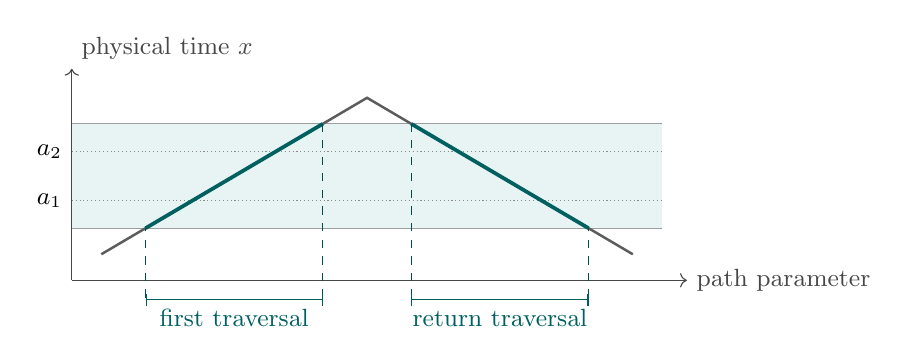
\begin{tikzpicture}[x=1.25cm,y=0.92cm,font=\small]
  \fill[teal!9] (0,0.72) rectangle (6.0,2.16);
  \draw[black!38] (0,0.72)--(6,0.72) (0,2.16)--(6,2.16);
  \foreach \y/\lab in {1.1/{a_1},1.78/{a_2}} {
    \draw[black!46,densely dotted] (0,\y)--(6,\y);
    \node[left] at (0,\y) {$\lab$};
  }
  \draw[->,black!72] (0,0)--(6.25,0) node[right] {path parameter};
  \draw[->,black!72] (0,0)--(0,2.92) node[above right] {physical time $x$};
  \draw[black!64,line width=.9pt] (.3,.36)--(3,2.52)--(5.7,.36);
  \draw[teal!75!black,line width=1.35pt] (.75,.72)--(2.55,2.16);
  \draw[teal!75!black,line width=1.35pt] (3.45,2.16)--(5.25,.72);
  \foreach \x/\y in {.75/.72,2.55/2.16,3.45/2.16,5.25/.72}
    \draw[teal!60!black,dashed] (\x,-.24)--(\x,\y);
  \draw[|-|,teal!75!black] (.75,-.27)--(2.55,-.27)
    node[midway,below] {first traversal};
  \draw[|-|,teal!75!black] (3.45,-.27)--(5.25,-.27)
    node[midway,below] {return traversal};
\end{tikzpicture}
\caption{Two visits to the same physical interval (shaded) occupy disjoint
parts of the path parameter. Each visit incurs a distinct interior break
for each tracer mark $a_1,a_2$. Only the time projection is drawn. A
break in a tracer coordinate need not be visible in that projection.}
\label{fig:return-traversals}
\end{figure}


\subsection{Nested episodes}
There are two depths in the construction. At level $j$, the clock and
resource inputs are systems from level $j-1$. Within a single level we
nest episodes in physical overlaps to depth $g_*$. This second depth
ensures that continuing through overlaps without taking an inner crossing
ultimately incurs just as many breaks.

Fix $K\ge2$ and $0<\eta<1$. For $N=L^h$, where the scheduler base $L$
will be fixed below, set
\[
  e=\frac{\eta}{200K},\qquad
  g_*=\lceil 2K/e\rceil,\qquad q_*=\lceil N^e\rceil .
\]
At each level the number $B_j$ of buckets must exceed four times the
label count $V$ times the dimension of the resource input. We allow
successively larger bucket counts by setting
\[
 b_K=\frac{e}{10g_*},\qquad b_{j-1}=\frac{b_j}{10g_*}\quad(3\le j\le K),
 \qquad B_j=\lceil N^{b_j}\rceil\quad(2\le j\le K).
\]
Set $J=1+\lfloor N^{b_2/8}\rfloor$. The integer multiplier $R\ge1$ controls
the number of marks and may be chosen independently of these parameters.

Write $Q_j(T)$ for a level-$j$ system on the signature $T$. At the top,
$T$ has one node. A level-$j$ driver on $T$ uses $Q_{j-1}(T)$ for its
clocks and $Q_{j-1}(T^+)$ for its resources. Since
Theorem~\ref{thm:scheduler} determines $T^+$ from $T$ before the client
program is chosen, all needed signatures are specified by descending
from the top. We now construct the systems in the opposite order.

At level one take a tracer with $RN$ distinct marked times in $(0,1)$.
At level $j\ge2$, every driver uses $B_j$ buckets and $q_*$ triples of
work windows. Label each overlap by its bucket and by its early or late
phase, giving the same alphabet of $2B_j$ labels in each episode. A word
in this alphabet records the successive overlaps in which an episode
is nested. Use one driver per word of length less than $g_*$.

The empty word indexes the driver with the $N$ prescribed disjoint
episodes in $(0,1)$. Once the driver for word $v$ is built, locate the
$i$th episode of the driver for $va$ strictly inside overlap $a$ of
the $i$th episode for $v$, for every $i$. Thus a child driver serves
all $N$ parent episodes. For $|v|=g_*-1$, choose $R$ distinct interior
times in each of its overlaps and put all these marks in one tracer.
The drivers and the tracer share $x$ and have separate coordinates.
Join their programs at $T$. This is $Q_j(T)$.

A viable set for the joined program restricts to a viable set on each
component. At fixed $x$ the tight coordinate matrix is block diagonal,
so its nullity on the usable coordinates of any component is at most
that of the whole matrix. Thus an admissible point projects to an
admissible point of each driver and of the tracer. In particular, every
viable set has more than $J$ coordinates, as required when $Q_j(T)$
itself becomes a driver input. The coordinate count below verifies
the bucket inequality at each level.

\begin{proposition}[Cost of a nested crossing]\label{prop:iterated-crossing}
Let $D_j=4^{1-j}RN^jq_*^{j-1}$. For all sufficiently large $N$, all
integers $R\ge1$, and all the signatures at level $1\le j\le K$, every segmentation
of an admissible crossing of $[0,1]$ in $Q_j(T)$ has at least $D_j$
segments. At levels $j\ge2$ every segmentation of an admissible traversal
of one empty-word episode has at least $D_j/N$ breaks in its parameter
interior. Both statements hold in either orientation.
\end{proposition}
\begin{proof}
The $RN$ marked times give the assertion for $j=1$. At level $j\ge2$ put
$A=D_{j-1}/2-1$ and fix a segmentation of the traversal. In any episode,
Lemma~\ref{lem:episode} supplies $q_*$ subpaths with disjoint parameter
interiors. Each either contains $A$ or more interior breaks or traverses
a designated overlap. In the latter case trim to the episode placed
inside that overlap. If this is a terminal overlap, use its $R$ tracer
marks instead. The segmentation induced by trimming has only original
breaks in its interior: the new endpoints never enter the count. This
remains true when two subpaths traverse the same physical overlap.

Let $E_t$ denote the lower bound obtained when $t$ driver levels remain
in this episode, counting the current driver. For a terminal overlap the
bound is $E_0=R$. Since a child charge is internal to its parent subpath,
the disjoint subpaths give the recurrence
\[
 E_t=q_*\min\{A,E_{t-1}\}
       =\min\{q_* A,Rq_*^t\}\qquad(t\ge1),
\]
where the second equality follows by induction. At the empty word
$t=g_*$. For large $N$ we have $D_{j-1}\ge4$, so $q_* A\ge
q_*D_{j-1}/4$. Also $q_*^{g_*}\ge N^{2K}\ge N^{j-1}q_*^{j-1}$
for $j\le K$ and sufficiently large $N$. Thus
\[
                     E_{g_*}\ge q_*D_{j-1}/4=D_j/N .
\]
Every full crossing has a traversal of each of the $N$ empty-word
episodes. Taking the first visit to the far endpoint and the last visit
to the near endpoint before it gives these traversals in order,
with disjoint parameter interiors. Hence the full crossing incurs
at least $D_j$ interior breaks and, in particular, at least $D_j$
segments.
\end{proof}

\subsection{Dimension and number of inequalities}
It remains to prove that the cost in inequalities grows by much less
than the factor $N$ gained in crossing length at each level. We track
three quantities: the number of coordinates used by the inputs, the span
of the support of each row, and the total number of rows. The first two
control how many buckets and how many choices of red slacks the next
level needs.

The choice of parameters is uniform in $R$. The depth $K$ and overhead
$\eta$ have already fixed $e,g_*$ and $b_2,\ldots,b_K$. The estimates
below impose two lower bounds on $r$. Once these are met, choose $L,V$
by Theorem~\ref{thm:scheduler} and then increase $N=L^h$. The multiplier
$R$ changes only the number of tracer marks and the coefficients needed
to realize the resulting schedules.

\paragraph{Coordinates.}
Let $H$ and $G$ denote the height and maximum outdegree of any signature
that occurs. Each passage to $T^+$ changes their bounds to $h+2H$ and
$10V(G+1)$. There are at most $K-1$ such passages, so
\[
 H\le C_K h,\qquad G+1\le(20V)^{C_K},\qquad
 |T|\le (G+2)^{H+1}\le N^{C'_K/r}.
\]
Indeed, $20V\le(10V)^2$ and $10V\le L^{3/r}$, so the logarithm of
$|T|$ is bounded by $C'_K h\log L/r$ with $C'_K$ independent of $r$.
Choose $r$ sufficiently large that $C'_K/r<b_2/16$. The span estimate below
will impose one further lower bound on $r$. Then $(J+1)|T|\le N^{b_2/4}$ for all
large $N$. This bounds the number of tracer coordinates regardless of
how many kinks are imposed.

We claim that the numbers $p_j$ of slice coordinates, uniformly over the
signatures at level $j$, satisfy
\[
     p_1\le N^{b_2/4},\qquad
     p_j\le N^{2g_* b_j}\quad(2\le j\le K).
\]
The first bound is the tracer estimate. Inductively the two inputs at
level $j$ each have at most $N^{b_j/4}$ coordinates, since
$2g_* b_{j-1}=b_j/5$ when $j\ge3$. In particular $B_j>4Vm$ for the
number $m$ of resource coordinates. A driver uses at most
$(10V+2) B_j N^{b_j/4}$ coordinates, counting the scheduler and its two
clock vectors per bucket. Its work windows reuse these coordinates.
There are at most $(2B_j)^{g_*}$ drivers, and a single further tracer.
The resulting coordinate exponent is at most
$(g_*+1+1/4)b_j+o(1)<2g_*b_j$. At level $K$, $2g_* b_K=e/5$, leaving
room for the time coordinate in the claimed dimension bound.

\paragraph{Span.}
A coupling row substitutes a red slack for each coordinate in the support
of a resource inequality. Bounding that support by the input dimension
would allow too many independent choices. Instead we show that every row
has span at most $C''_K h+O_{K,r,L,V}(1)$ with $C''_K$ independent of $r$.

An individual bound has span at most $H+1$ and a scheduler row has span
$O(h+H)+O_{r,L,V}(1)$, with an absolute constant in the first term.
In a coupling row the two upper inequalities contribute at most two input
spans, allowing also individual bounds and caps. For a resource row of
span $s$, the union of the supports of its chosen red rows has span at
most $5s$ by Theorem~\ref{thm:scheduler}. Joining the programs adds no
request ancestors, so this calculation passes to their union. Induction
over the fixed $K$ levels gives the claimed span bound, independently of
the number of marks. Support size is at most span. Since there are at
most $2V$ red rows available at each supported request, expanding the
minima costs at most
\[
        (2V)^{C''_K h+O_{K,r,L,V}(1)} \le N^e .
\]
For this final inequality choose $r$ also large enough that $3C''_K/r<e$,
then fix $L,V$ from Theorem~\ref{thm:scheduler}, and take $h$ sufficiently
large. This order meets both requirements on $r$.

\paragraph{Rows.}
Let $F_j$ be the maximum number of affine rows at level $j$. We prove
\[
                     F_j\le R N^{1+20je}.
\]
For large $N$, each of the number of drivers, the bucket count, the number
of tracer coordinates and either input dimension is at most $N^e$. At
level one, each tracer coordinate uses $RN+1$ rows. At subsequent levels
there are at most $(\#\text{drivers})\,2B_j N R$ kink marks. Thus all
tracer rows together cost at most $R N^{1+4e}$. The ordinary
time-dependent clock floors use $O(N)$ affine pieces per coordinate.
Including all drivers and buckets their count is at most $N^{1+4e}$.
By Theorem~\ref{thm:scheduler}, the retained scheduler rows in all
drivers cost at most
\[
 O_{r,L,V}\!\left((\#\text{drivers})\,N B_j m
                         (1+(B_jm)^2)\right)\le N^{1+8e}.
\]

The coupling rows are where a product of input row counts could occur.
In a given bucket, each of the three overlays contributes at most
$q_*F_{j-1}$ input-copy choices and $O(q_* N^e+1)\le N^{3e}$ choices
of blanks and caps. Lemma~\ref{lem:coupling} permits us to delete every
triple containing two or more input-copy rows. There are consequently at
most
\[
                 N^{9e}+3q_*F_{j-1}N^{6e}
\]
retained triples per bucket before expanding minima. The first term counts
triples of blanks and caps, and the factor three in the second chooses the
overlay contributing the single input-copy row. The number of drivers,
the buckets per driver and the expansions per triple each cost at most
$N^e$. As $q_*\le2N^e$, all coupling rows together cost at most
$N^{12e}+6F_{j-1}N^{10e}$. The tracer, clock and scheduler counts above
now give $F_j\le RN^{1+20je}$ by induction. The tracer cost is linear
in $R$, and no product of two input row counts survives. All thresholds
on $N$ can therefore be taken independent of $R$.

\begin{proof}[Proof of Theorem~\ref{thm:seed}]
At the top take the one-node signature. The construction now has
$F_K+3\le R N^{1+\eta}$ and $p_K+1\le N^\eta$. Every crossing on fixed-time
slice faces of dimension at most $J$ is admissible, by
Definition~\ref{def:admissible}. Proposition~\ref{prop:iterated-crossing}
gives at least $RN^K(q_*/4)^{K-1}$ segments on a full crossing and
$RN^{K-1}(q_*/4)^{K-1}$ interior breaks on each admissible traversal of a complete outer
episode. Since $q_*\ge4$ for large $N$, these bounds imply $RN^K$ and
$RN^{K-1}$, respectively. Taking $\gamma=b_2/8$ gives $J=1+\lfloor N^\gamma\rfloor$,
as required in Theorem~\ref{thm:seed}. The coefficients of the system
may depend on $R$ and on the chosen times.
\end{proof}

\section{Numerical states that distinguish time intervals}\label{sec:numerical}

The scheduler uses the same coordinates in many disjoint intervals.
Each interval must have a recognizable set of coordinates at zero. It
must also be possible to interpolate between successive samples using
convex inequalities. We construct finite sets of nonnegative vectors
that meet both requirements.

Call the intervals \emph{sites}, and number them from \(1\) to \(L\).
A \emph{layer} is a sample position in their linear order. Each site
has a blank layer at either end and any positive number of intervening
layers, called \emph{micro layers}. The last blank of one site and the
first blank of the next are distinct.

\begin{theorem}[Numerical layer theorem]\label{thm:coarse}
Fix integers \(r\ge100\) and \(C\ge1000r^2\). There are arbitrarily
large powers of two \(q\) with the following property. Set \(L_0=q^C\)
and \(L=L_0^m\) for any sufficiently large integer \(m\). Let \(b\)
be the least power of two at least \(L^{1/(r+1)}\), and let
\(\mathcal A\) be a nonempty set of at most \(b\) positions.
There are a finite index set \(\mathcal I\) and maps
\(\mathrm h_a:\{1,\ldots,L\}\to\mathbb F_b\) for \(a\in\mathcal A\)
such that
\[
 |\mathcal I|\le L^{8/C},\qquad
 \big|\{a:\mathrm h_a(s)=\mathrm h_a(s')\}\big|\le r
 \quad(s\ne s').
\]
Index coordinates by labels \(\ell=(i,a,t)\) in
\(\mathcal I\times\mathcal A\times\mathbb F_b\). The \emph{bundle}
with index \(i\) at site \(s\) is
\(H_i(s)=\{(i,a,\mathrm h_a(s)):a\in\mathcal A\}\).
For any numbers of micro layers, each layer \(j\) admits a finite
nonempty set \(\mathcal S_j\) of vectors in the unit cube on these
labels, called \emph{states}, with the following properties.
\begin{enumerate}
\item Given states \(u\in\mathcal S_{j-1}\) and
\(v\in\mathcal S_{j+1}\) on either side of any layer \(j\), some
\(y\in\mathcal S_j\) satisfies
\begin{equation}\label{eq:layermerge}
                y_\ell\le\tfrac14\max\{u_\ell,v_\ell\}
                \quad\text{at every label }\ell .
\end{equation}
\item Every state at a micro layer of site \(s\) vanishes on one
entire \(H_i(s)\). On each \(H_{i'}(s')\) with \(s'\ne s\) it has
at most \(r\) zero coordinates.
\item The number of states per layer is bounded independently of all
site lengths. If there are \(n_L\) layers, every positive state entry
has the form \(4^{-k}\) for an integer \(0\le k\le c_0 n_L\);
\(c_0\) may depend on \(r,C,q,m,\mathcal A\).
\end{enumerate}
\end{theorem}

The coordinates will record how often a path changes direction while
avoiding a specified label. To see what paths are needed, imagine
building a state at each layer and repeatedly adjoining the states
required by Equation~\eqref{eq:layermerge}. A binary expression
records the history of each such operation.

\subsection{Binary terms and a one-scale marking lemma}

A \emph{term} is a finite rooted binary expression with a layer
assigned to each node. Each layer has a leaf term. At an interior
layer a new term can be formed by merging any term in the preceding
layer (its west parent) with any term in the following layer (its
east parent). These rules generate all terms. A path follows parent
links and includes both its endpoints. A \emph{turn} is a change of
direction between consecutive links. The west and east \emph{spines}
of a term follow the respective parent at each step until a leaf is
reached.

We will also use terms on a contiguous block of layers. To \emph{clip}
a term to a block containing its root, replace each node first reaching
either boundary layer of the block by the leaf in that layer. The paths
of the clipped term follow the same parent links as in the original
term up to their endpoints. On such a path, clipping the original
subterm at any visited node gives precisely its subterm in the clipped
expression.

The next lemma provides a random mark on a fixed number \(L_0\) of
sites. Every micro term receives the mark with a specified minimum
probability. From any blank term there is a path to a leaf that
encounters the mark in at most one other site. Sections~\ref{sec:probability}--\ref{sec:finite}
give the construction and proof.

\begin{lemma}[Primary Lemma]\label{lem:primary}
For each integer \(C\ge50\) there are arbitrarily large powers of two
\(q\) with the following property. For \(L_0=q^C\) sites there is a
finite probability space \(\Omega\) independent of the numbers of
micro layers. For any choice of those numbers, each term \(v\) can
be assigned a set \(P(v)\subseteq\Omega\) such that
\begin{enumerate}
\item \(P(v)=\varnothing\) on every blank layer and
\(\Pr(P(v))\ge q^{-5}\) on every micro layer.
\item For every blank term in site \(s\) and every \(\omega\in\Omega\),
there is a path from that term to a leaf on which all terms \(v\)
with \(\omega\in P(v)\) lie in a single site different from \(s\).
There may be no such terms. The number of turns is bounded in terms
of \(C,q\) alone.
\end{enumerate}
\end{lemma}

\subsection{Distinguishing sites at successive scales}

Choose \(q\) from Lemma~\ref{lem:primary} large enough that
\(2\log_2 L_0\le q\). Partition the \(L=L_0^m\) sites into blocks
of \(L_0\) consecutive sites. Group \(L_0\) consecutive blocks into
a larger block, repeating until the entire sequence forms one block.
Number the levels from \(1\) to \(m\), starting with the finest blocks.
At each level above the first, a site is a whole block from the previous
level. Regard its first and last layers as blanks and all intervening
layers as micro layers. Apply the Primary Lemma to the \(L_0\) sites
in every block, clipping terms to that block. A term \(v\) on a finest
micro layer is micro at every level and thus has \(m\) sets of marks of
measure at least \(q^{-5}\).

There is a fixed list \(\mathcal T\subseteq\Omega^m\) of size at most
\(q^{7m}\) that meets every product of \(m\) subsets of \(\Omega\)
whose individual measures are at least \(q^{-5}\). Indeed, \(q^{7m}\)
independent tuples sampled from the product measure miss any such
product with probability at most \(\exp(-q^{2m})\). There are at most
\(2^{m|\Omega|}\) products. Since \(\Omega\) was fixed before \(m\),
their total failure probability is less than one for all sufficiently
large \(m\).

Within each block write its site numbers \(0,\ldots,L_0-1\) in binary,
using \(\log_2 L_0\) bits per number. An index \(i\) consists of a
tuple in \(\mathcal T\) and, for each level, a bit position and a bit
value. Thus the set \(\mathcal I\) of possible indices satisfies
\begin{equation}\label{eq:tensor-index-size}
        |\mathcal I|\le q^{7m}(2\log_2 L_0)^m
        \le q^{8m}=L^{8/C}.
\end{equation}
We assign one index to each finest micro term and none to the finest
blank terms. We say that a term \emph{emits} its assigned index.
At every level the tuple entry of an emitted index must be a mark of
the clipped term, and the recorded bit must match the address of its
site. We now choose the bits so that these two necessary conditions
exclude repeated emissions along a suitable path.

\begin{lemma}\label{lem:emission-escape}
The assignment can be made so that from every term emitting \(i\)
there is a path to a leaf on which all emissions of \(i\) occur in
its starting finest site. The number of turns on this path is bounded
independently of the term and the site lengths.
\end{lemma}
\begin{proof}
At a finest micro term \(v\), choose a tuple from \(\mathcal T\)
belonging to all \(m\) sets of marks. Follow one spine in the starting
site as far as a leaf or the first blank. If a blank is reached, apply
Lemma~\ref{lem:primary} there in the level-one block, with the first
entry of the tuple. On the resulting path all occurrences of that mark
lie in a single different site. Choose a bit where the addresses of the
two sites differ, and record the starting site's value. If the mark
never occurs, any position with its correct value suffices. On this
segment a term therefore either lacks the required mark or fails the
bit test. Figure~\ref{fig:layer-bits} illustrates the choice.

Lift the path from the clipped term to the original term. If the endpoint
is a genuine leaf, stop. Otherwise it is an exterior blank of the
level-one block, and therefore a blank of the starting site at level two.
Repeat with the next tuple entry. The preceding clipping observation
ensures that the marks tested on a lifted segment agree with the ones
used to decide whether its terms may emit the index. At the last level
an exterior blank is a global endpoint and necessarily a genuine leaf.
For any unused levels record an arbitrary correct bit. The initial
spine stays within the starting finest site, and each subsequent
segment excludes the index. There are at most \(m\) such segments,
each with the bounded number of turns from the Primary Lemma, and at
most \(m\) joining turns. The choices at \(v\) depend only on addresses
and marks, so they can be made at every micro term independently.
\end{proof}

\begin{figure}[htbp]
\centering
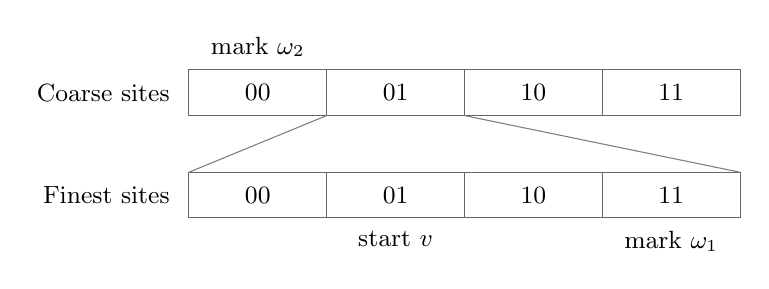
\begin{tikzpicture}[x=1cm,y=1cm,font=\small]
  \foreach \j/\bits in {0/00,1/01,2/10,3/11}{
    \draw[black!60] ({1.75*\j},1.3) rectangle ({1.75*\j+1.75},1.88);
    \draw[black!60] ({1.75*\j},0) rectangle ({1.75*\j+1.75},.58);
    \node at ({1.75*\j+.875},1.59) {\(\bits\)};
    \node at ({1.75*\j+.875},.29) {\(\bits\)};
  }
  \node[anchor=east] at (-.12,1.59) {Coarse sites};
  \node[anchor=east] at (-.12,.29) {Finest sites};
  \draw[black!50] (1.75,1.3)--(0,.58);
  \draw[black!50] (3.5,1.3)--(7,.58);
  \node[anchor=south] at (.875,1.92) {mark \(\omega_2\)};
  \node[anchor=north] at (2.625,-.05) {start \(v\)};
  \node[anchor=north] at (6.125,-.05) {mark \(\omega_1\)};
\end{tikzpicture}
\caption{Choosing an address bit at each of two levels. Within the
starting coarse site \(01\), the finest site of \(v\) is \(01\) and
the first mark occurs only in \(11\) along the first escape segment.
Recording the first bit of \(01\) excludes \(11\). On the next
segment the second mark occurs only in coarse site \(00\). The second
bit of the starting coarse site \(01\) excludes its entire block.}
\label{fig:layer-bits}
\end{figure}

\subsection{Numerical slack from paths}

Assign distinct polynomials of degree at most \(r\) over \(\mathbb F_b\)
to the \(L\) sites, and evaluate each polynomial at distinct field elements
indexed by \(\mathcal A\) to obtain the tags \(\mathrm h_a(s)\). This is
the polynomial evaluation construction of Reed and Solomon~\cite{reedsolomon}.
There are \(b^{r+1}\ge L\) polynomials, and two distinct polynomials agree
at at most \(r\) positions. Whenever a term at site \(s\) emits \(i\),
regard it as emitting each label in \(H_i(s)\).

\begin{proof}[Proof of Theorem~\ref{thm:coarse}]
For a term \(v\) and label \(\ell\), consider all paths from \(v\) to a
leaf that avoid emission of \(\ell\) at every term, including \(v\).
A path of zero steps has cost zero. For a nonempty path \(\pi\), write
\(\partial_\pi\) for the global boundary layer in the direction of its
first step and define
\begin{equation}\label{eq:turn-cost}
 c(\pi)=1+\operatorname{dist}(v,\partial_\pi)
                   +3n_L\,\operatorname{turns}(\pi),
\end{equation}
where distance counts layer steps. Prepending a step increases the cost
by at least one. In the original direction the distance increases by one.
In the opposite direction a new turn contributes \(3n_L\), exceeding any
loss in the distance term. Prepending to an empty path also increases
the cost.

Choose \(c_0\) so that the cutoff \(c_0 n_L\) bounds the cost of a
spine followed by a path from Lemma~\ref{lem:emission-escape}, including
the turn at the join. The lemma bounds the number of turns independently
of \(n_L\). If the minimum cost of an avoiding path is \(k\le c_0 n_L\),
put \(y_\ell(v)=4^{-k}\). If there is no such path below or at the cutoff,
put \(y_\ell(v)=0\). Let \(\mathcal S_j\) consist of the vectors \(y(v)\)
of all terms in layer \(j\). Each layer has a leaf, so its set is
nonempty. At a fixed layer the first direction has two choices and the
number of turns below the cutoff is bounded in terms of \(c_0\). Thus
Equation~\eqref{eq:turn-cost} allows only boundedly many exponents for
each coordinate. The number of labels is independent of the site
lengths, giving the asserted uniform state count.

Given states at the two neighbors of a layer, merge terms carrying those states.
A positive entry \(4^{-k}\) of the merge has an avoiding path of cost
\(k\). Removing its first step gives one parent an avoiding path of cost
at most \(k-1\), so that parent's entry is at least \(4\cdot4^{-k}\).
Thus the merged vector satisfies Equation~\eqref{eq:layermerge}. At a
micro term its own emission cannot be avoided, so the state vanishes on
the entire emitted bundle.

Finally fix an index \(i\) and a micro term at site \(s\). If a spine
from the term reaches a leaf without an emission of \(i\), that one
path avoids every label with first component \(i\) within the cutoff.
Otherwise denote the sites of the first emissions on the west and east
spines by \(s_-\) and \(s_+\). At the first emission on each spine,
continue along the path of Lemma~\ref{lem:emission-escape}. The new
paths stay below the cutoff and can encounter labels of index \(i\)
only in \(H_i(s_-)\) and \(H_i(s_+)\), respectively. Every zero of
index \(i\) therefore lies in \(H_i(s_-)\cap H_i(s_+)\). If either
site equals \(s\), its intersection with a foreign bundle contains at
most \(r\) labels by polynomial evaluation. Otherwise \(s_-\) is
strictly west of \(s\) and \(s_+\) strictly east, so even
\(H_i(s_-)\cap H_i(s_+)\) has at most \(r\) labels in total.
\end{proof}

\section{Directional coverage and small cuts}\label{sec:probability}

Lemma~\ref{lem:primary} requires frequent occurrences on the micro
layers and, from each blank term, a path along which all occurrences lie
at a single other site. To see how the two requirements fit together,
assign each micro term a color and associate it with one blank term on
each shore of its site. These two blank terms are its \emph{keys}. An
outcome selects a color and opens certain keys in that color. An
occurrence requires a term of the selected color with both keys open.

Follow the outward spine from a blank term. If it encounters an
occurrence, then at that site it also encounters an open key in its
direction of travel. It suffices, from the first such key, to find a
continuation to a leaf whose moves charge no open key outside that
site. The rules below encode this condition in a graph that compresses
each straight run of parent steps into one move. A move \emph{charges}
its direction key if the run could contain a term of the selected color.
Thus every occurrence encountered on the run forces a charge to an
open key in the occurrence's site.

The proof builds the rules on a nested sequence of intervals. Within
one interval and for a fixed color, a collection of successful keys
\emph{covers} a test if it is charged on every short path towards one
end of the interval. Low probability of coverage supplies the desired
continuations. This section bounds the weight of the small sets of keys
that can cover such a test and orders typical pairs of those sets. In
Section~\ref{sec:switching} that order will allow the preferred direction
to change as the interval grows. Section~\ref{sec:finite} realizes the
rules on terms using a finite probability space.

\subsection{Moves, colors and path tests}

The sites are the integers from $1$ to $L_0$, in their usual order.
We work in a directed acyclic graph of bounded outdegree. The graph may
be infinite. Write $m(v)$ for the site of a node $v$. A node is either
a \emph{micro node} or a \emph{blank node} on the west or east shore of its site. The
blank nodes are also called \emph{keys}. We say that $u$ reaches $v$ if
there is a finite directed path from $u$ to $v$, allowing the empty path.
We call every node reachable from $u$ an ancestor of $u$.

A blank leaf has no moves. From any other blank node there are two
basic moves. The outward move leads to a blank on the facing shore of
the adjacent site, and the inward move leads to a micro node in the
same site. Thus a blank node with no neighboring site across its shore
is a leaf. Each micro node has a basic move in either direction, leading
to a key on the corresponding shore of its own site, its
\emph{direction key}. It may also have jumps in that direction to
other micro nodes in its site. Every such jump preserves the direction
key. A \emph{spine} follows basic moves in one geographical direction
until it reaches a leaf or leaves the interval being tested. At most
three of its moves originate at a given site, and it visits at most
one micro node there.

The graph is revealed in rounds. All micro nodes have the same color
in round zero. At each later round, a deterministic rule assigns a
shore to each old color. A micro node appends to its old color a datum
computed at its key on that shore. Once these colors have been
calculated, the round supplies flags and witness jumps subject to the
following rules.
\begin{enumerate}
\item For each micro node, direction and color there is a flag. When
the flag is true, every move from that node in that direction charges
its direction key in the specified color. All other moves carry no
charge in that color. In particular a blank node never charges a key.
\item A true flag in a refined color requires a true flag in the same
direction for its projection to the preceding round.
\item Each true flag has a witness of the specified color, either the
micro node itself or a micro node reached by one jump in that
direction. The round adds at most one such jump per node, direction
and color. All earlier moves remain available.
\end{enumerate}
All flags, witnesses and calculated colors are independent of the
randomness used for the gates. In the application to free terms, a basic
move from a micro node compresses travel through several micro layers.
Its flags record the colors encountered there, and the witness jumps
recover individual occurrences. A refinement can add paths
and can remove charges when an old path is read in the refined color.
At a charging move we may always use the basic move to the charged key
instead, with the same charge. Alternatively we may reach the witness
from the source of the charging move in at most one move.

For a cluster (an interval of sites), a \emph{west test at $v$ to depth
$e$} consists of all paths from $v$ inside the cluster to a leaf or
through their first west exit. The number of moves originating at any
one site is at most $e$, including the exiting move. We also use
depth vectors, with a separate bound for each site. East tests are
defined by reflection. A set of keys \emph{covers} a test in a color if
every tested path charges some key in the set in that color. Random
\emph{coverage} means coverage by the keys whose gates in that color
succeed. Each test of finite depth is finite, since path length is bounded
by the sum of the depths and branching is bounded.

Two observations account for the depth bounds below. A depth is
charged to the \emph{source} of a move. Thus replacing a charging jump
by the basic move to its direction key preserves both the charge and
the depth spent at each site. Also, suppose a path prefix from \(v\)
to \(u\) stays in the cluster, avoids charges to a set \(B\), and spends
at most \(b_x\) moves at each site \(x\). If \(B\) covers the west test
at \(v\) to depth vector \(f\ge b\), then \(B\) covers the west test at
\(u\) to depth \(f-b\). Prepending the prefix to a missed path at \(u\)
would give a missed path at \(v\). This applies whatever directions
the prefix follows. Enlarging a depth only enlarges the set of test
paths. Thus a covering set also covers every shallower test, and a
path witnessing failure of coverage persists in every deeper test.

A rule at a key is \emph{local} if it reads a bounded outgoing unfolding
at that key, with the types of the nodes, their sites, flags, labeled
move slots and the equality relation on nodes in the unfolding. The
radius may depend on the parameters of the construction. A rule
refining a color sees only flags and moves already supplied.
The independent random bits read by a gate are indexed by keys or
bounded nonempty sets of keys in the unfolding, with auxiliary indices
such as stages and colors. Different appearances of the same index refer
to the same bit. Both the radius and the number of slots are uniformly
bounded once the parameters are fixed.

\subsection{The induction and its screens}

Fix an integer $C\ge 50$ and put
\begin{equation}\label{eq:prob-parameters}
 \begin{gathered}
 K=4C,\quad J=10000K\,4^K,\quad w=3J,\quad h=Cw,\\
 q=a^w,\quad L_0=a^h=q^C,\quad t=a^{-J},\quad U=at,\quad z=a^{-1/C}.
 \end{gathered}
\end{equation}
Here $a$ is a sufficiently large power of $2$ that is a perfect
$C$th power. Fix a constant $\lambda>0$ with
$K\exp(-\lambda/5)<1/4$. Constants in the estimates can depend on $C$
and $\lambda$. Bounds of the form $a^{o(1)}$ are uniform in the graph.

At stage \(i\), \(0\le i<h\), partition the sites from left to right
into successive clusters of \(a^i\) sites. Each cluster after stage
zero has \(a\) children from the preceding partition. Two rounds of
refinement at each positive stage assign each color a direction.
Within each cluster a key's gate uses only bits indexed in that cluster.

The induction asserts that for every node and color the probability of
coverage to per-site depth \(D_i\) in its assigned direction is at most
\(t\). Here \(D_i\ge4\) and the number of colors are polylogarithmic
in \(a\), since \(C\) and hence \(h\) are fixed. We need the same bound
after choosing any collection of \emph{ignored sites}. Fix the raw
bits at their keys arbitrarily and count only charges originating
outside those sites. All other bits retain their prescribed laws.

There is an independent raw bit at each key at each stage, shared by all
colors. At stage $0$ the gate is the raw bit, of success probability
$q^{-1}$. Assign the unique color the west direction and take $D_0=4$.
The west spine in a single site has at most one charge, so the initial
coverage probability is at most $q^{-1}\le t$, also with ignored sites.
At each positive stage a gate retains the requirements of its projected
color and adds three requirements. Its new raw bit must succeed (with
probability $z$), its \emph{screen} must pass, and a specified collection
of independent \emph{barrier bits} must all succeed. The screen uses
only randomness of previous stages. The barrier indices depend
deterministically on the key and color. The construction will give a
joint passage probability of at least $\exp(-4\lambda)$ for the
barriers at any one key and color at that stage.

Fix a positive stage $i$ and an old color (the color after stage $i-1$).
Reflect the sites, and the coordinate $m(v)$ if necessary
so that the old direction is west. Put \(d=D_{i-1}\). In a new cluster the old probability of west
coverage to depth \(d\) is at most \(U=at\), including under the
conditioning on ignored sites. Start in the child containing the
given node. Unless the test there is covered, choose a missed path
using only that child's bits. It either terminates at a leaf or exits
into the adjacent child to the west. In the second case apply the
same rule from the new starting node. Its location is determined
before any bits of the new child are inspected. Thus the conditional
probability of coverage at each step is at most \(t\). The visited
children are distinct, so concatenating the paths respects every
per-site depth. A union bound over at most \(a\) children proves
the estimate.

At a key $g$, let $A_g$ be old west coverage from $g$ in the new cluster
to depth $d$ with $g$'s own site ignored. In particular
$\Pr(A_g)\le U$ even conditional on arbitrary raw bits at its site.
A \emph{pin} at a key means that its raw bits have all succeeded through
stage $i-1$. Pins at distinct keys are independent, each with probability
\[
 p=q^{-1}z^{i-1}.
\]
For a set of keys $S$ we write $[S]$ for the event that all its pins are
present. Put $\alpha_j=U^{1/4^j}$ for $0\le j\le K$. The screen at $g$
fails if $A_g$ occurs or if
\begin{equation}\label{eq:pin-screen}
 [S]\text{ occurs for some } |S|\le K
 \text{ with }\Pr(A_g\mid [S])>\alpha_{|S|}.
\end{equation}
Passing the first part of the screen guarantees a missed path from
\(g\). Passing the second means that exposing a small set of successful
pins cannot make the absence of such paths too likely. The second test
is local as well. The event \(A_g\) depends on only finitely many local
bits. Removing pins outside that dependence leaves the conditional
probability unchanged and can only lower the threshold. Thus it
suffices to check sets \(S\) of local keys. For the rest of this
section a \emph{screened success} means that the old gate succeeds
and the current screen passes. The thinning and barrier bits of the
current stage enter in Section~\ref{sec:switching}.

\begin{lemma}[Conditional cost of a screen]\label{lem:pcost}
Suppose that a bounded set $P$ of keys satisfies
$\Pr(A_g\mid[S])\le\alpha_{|S|}$ for each $S\subseteq P$ with
$|S|\le K$. Conditional on $[P]$, the probability of
\eqref{eq:pin-screen} is $O_{|P|}(\alpha_K)$.
The same bound holds for failure of the whole screen if also
$\Pr(A_g\mid[P])\le\alpha_K$, as holds whenever $|P|\le K$.
\end{lemma}

\begin{proof}
Let $X_1,\ldots,X_N$ be independent Bernoulli variables with success
probability $p$, and $E$ an event, possibly using additional randomness,
with probability $\mu$. For $u>0$ and $u\ge2\mu$, the probability that
some set of at most $K$ present successes raises the conditional
probability of $E$ above $u$ is at most $4^{K+1}\mu/u^2$. To see this,
expand $\Pr(E\mid X_1,\ldots,X_N)$ in the orthonormal product basis
whose one-coordinate factor is $(X_j-p)/\sqrt{p(1-p)}$
\cite[Sections~8.1 and~8.4]{Odonnell2014}. The constant
coefficient is $\mu$, and the sum of squares of the coefficients is at
most $\mu$ by conditional Jensen's inequality. Conditioning a proposed
set $T$ to succeed kills all terms indexed outside $T$. Each surviving
factor is at most $p^{-1/2}$ in absolute value. If the conditional
mean exceeds $u$, some nonempty $I\subseteq T$ therefore has coefficient
of magnitude at least $2^{-K-1}u p^{|I|/2}$. Sum
$\Pr([I])=p^{|I|}$ over the sets with such a coefficient and apply the
sum-of-squares bound.

Now suppose \(T\) witnesses~\eqref{eq:pin-screen}, and put
\(S=T\cap P\), \(j=|S|\). The hypothesis rules out \(T\subseteq P\),
so \(j<K\). First condition on \([S]\). The pin indicators outside
\(P\) still form a product measure, and the conditional probability
of \(A_g\) is at most \(\alpha_j\). The outside pins of \(T\) raise
this probability above \(\alpha_{|T|}\ge\alpha_{j+1}\).
For fixed \(S\), the event that some such outside pins are present
depends only on their indicators: the conditional probabilities
used to decide which sets qualify are deterministic numbers. Hence
the further conditioning on \([P]\) leaves the probability of this
event unchanged. The product-measure estimate with
\(u=\alpha_{j+1}\ge2\alpha_j\) bounds it by
\[
 O_K\bigl(\alpha_j/\alpha_{j+1}^2\bigr)
   =O_K\bigl(\alpha_{j+1}^{\,2}\bigr)=O_K(\alpha_K).
\]
Summing over \(S\subseteq P\) proves the first assertion. The
additional hypothesis bounds the cost of \(A_g\) itself.
\end{proof}

\begin{lemma}[Joint screened successes]\label{lem:joint-gates}
If $k\le K$ distinct keys can all have screened success in the old
color, their probability of doing so is at least $\gamma p^k$, where
$\gamma=\tfrac12\exp(-8\lambda hK)$. The bound also holds if, in
addition, one independently resamples all raw bits at any one site and
requires the keys at all other sites to retain screened success.
\end{lemma}

\begin{proof}
Condition on the $k$ pins. At every required screen, joint possibility
implies that none of the deterministic conditional-probability tests on
subsets of these pins violates its threshold. For a screen of an earlier
stage this applies to the corresponding earlier pins. Later raw bits are
independent of its inputs. Lemma~\ref{lem:pcost} consequently bounds the
conditional failure probability at each screen by $O_K(\alpha_K)$,
using the same $U$ in all stages. Every barrier requires positive
values of specified bits independent of the raw bits. Overlaps in these
requirements can only increase their joint probability above the product
of their individual passage probabilities, so all pass with conditional
probability at least $\exp(-4\lambda hK)$.

For the second assertion, keep the barrier bits fixed and independently
resample all raw bits at the chosen site. The only imposed pins in this
new environment are those outside that site. Every subset of them
passed the same deterministic tests under the original possibility
assumption. The conditional failure bound therefore applies to the
additional screens as well. Their barrier requirements use exactly the
original indices and bits. Conditional on the pins, all barriers pass
with probability at least \(\exp(-4\lambda hK)\). Subtract the
conditional failure probabilities of at most \(2hK\) screens.
This subtraction requires no independence between screens and
barriers. For large \(a\) the remaining probability is at least
\(\gamma\). Multiplying by the original pin probability \(p^k\)
proves both claims.
\end{proof}

\subsection{The weight of minimal cuts}

When a set of keys covers a test, every permitted path charges at least
one of those keys. To bound the probability of coverage by successful
keys, we count small covering sets that remain minimal when the depth
is reduced.
We require the two depths because concatenating a prefix uses up part
of the depth budget.

Choose the old moves and color, or the moves and a refined color after
either round of the current stage. Keep this choice fixed when testing
coverage. In every case the success probability is measured using
the screened gates for the \emph{old} color. Given per-site depths
\(d\le e\), \(e+d\le f\), with \(\max f=a^{o(1)}\), form the
\emph{\((e,f)\) list} at \(v\) of all sets \(B\) of at most \(K\) keys
satisfying three conditions.
\begin{enumerate}
\item \(B\) covers the west test at \(v\) to depth \(f\).
\item No proper subset of \(B\) covers it to depth \(e\).
\item The keys in \(B\) can have simultaneous screened success.
\end{enumerate}
The depth inequalities are componentwise when \(e,f\) are vectors.
The west spine ensures that \(B\) is nonempty. For each \(b\in B\),
a path missed by \(B\setminus\{b\}\) to depth \(e\) must charge \(b\),
so every listed key occurs in the local unfolding. In particular the
list is finite and is determined before the bits are sampled. Assign
each set the weight \(r(B)=p^{|B|}\), the probability of its pins.
The next lemma bounds both the total weight and the weight of all
strict extensions of a fixed nonempty set \(S\).

\begin{lemma}[Mass and link of a list]\label{lem:cut-list}
For every $(e,f)$ list $\mathcal L$ and every nonempty set $S$ of keys,
\[
 \sum_{B\in\mathcal L}r(B)\le aU,
 \qquad
 \sum_{\substack{B\in\mathcal L\\ B\supsetneq S}}r(B)
       \le a^{-500K}r(S).
\]
\end{lemma}

\begin{proof}
First we bound the number of cuts on the list that can succeed in
one outcome. Fix the bits and call a key available if it has screened
success. Further keys may be excluded arbitrarily. Let \(S\) contain
at most \(K\) available keys and suppose it fails to cover to depth
\(e\). We construct at most
\begin{equation}\label{eq:cut-branch}
 K\max e+1+d
\end{equation}
candidate keys outside \(S\). Every extension of \(S\) by available
keys that covers to depth \(f\) must contain a candidate, whatever
the cardinality of the extension.

Choose a depth-$e$ path $P$ missed by $S$. Offer all available keys it
charges at sites of $S$, at most $K\max e$ in number. For extensions
using none of these keys, exclude them for the rest of this step. Take
the first charge along $P$ to any remaining available key $g$. If there
is none, no such extension covers $P$. Otherwise $g$ lies at a site
unused by $S$. Its screen guarantees an old depth-$d$ west path from
$g$ missed by the old successes outside its site. Follow $P$ up to the
charge, redirect the charging move to $g$, and append this missed path.
The result is a west test path of depth at most $e+d$ in the selected
round. The prefix before the charge avoids every still eligible extension,
and the appended old path can only lose charges under refinement.
The extension must therefore use $g$ or a key charged on the appended
path at $g$'s site. Offering these at most $1+d$ possibilities proves
\eqref{eq:cut-branch}.

Branch from the empty set until $K$ keys have been chosen or the
depth-$e$ test is covered. In the latter case minimality forces any
listed extension to equal the current set. Consequently
at most $M=(K\max e+d+2)^K=a^{o(1)}$ cuts on the list can succeed
simultaneously. For any subfamily $\mathcal F$ let $E_B$ denote either
screened success of $B$ or its joint success with one-site resampling
as in Lemma~\ref{lem:joint-gates}. Counting the successful sets gives
\begin{equation}\label{eq:cut-multiplicity}
 \gamma\sum_{B\in\mathcal F} r(B)
 \le \mathbb E\sum_{B\in\mathcal F}{\bf 1}_{E_B}
 \le M\Pr\Bigl(\bigcup_{B\in\mathcal F}E_B\Bigr).
\end{equation}
Even one successful cut implies old coverage to depth $d$, since all
old paths of that depth remain available and old charges include their
refined charges. The union probability for the full list is at most $U$,
giving the mass bound.

For the link bound suppose the family of strict extensions of $S$ on the
list is nonempty. By minimality there is a depth-$e$ path $P$ missed by
$S$. Fix one independently of the bits. The keys it charges at sites of
$S$ are all outside $S$, at most $K\max e$ in number. Conditional on
$[S]$, the probability that at least one has a pin is at most
$K(\max e)p$. For the extensions using such a key, the union of the success events
requires both $[S]$ and an extra pin on the path. By
\eqref{eq:cut-multiplicity} their weight is at most
$M K(\max e)p\,r(S)/\gamma$.

Let $\mathcal R$ be the family of remaining extensions. If it is
nonempty, let $g$ be the first key in $\bigcup_{B\in\mathcal R}B$
charged along $P$. Thus its site is free of $S$, the prefix
before its charge misses the whole family, and some member contains
$S\cup\{g\}$. Possibility for that member implies
$\Pr(A_g\mid[S])\le\alpha_{|S|}$ by the screen at $g$.
Independently resample all raw bits at $g$'s site, recomputing every
gate and screen with these replacements. Conditional on the
original pins $[S]$, the same bound on $A_g$ holds in the resampled
environment. Unless $A_g$ occurs there, choose a missed old path from
$g$ to depth $d$, using the resampled environment. For $B\in\mathcal R$
let $E_B$ denote the joint event of Lemma~\ref{lem:joint-gates},
including resampling. If $E_B$ occurs, $B$ must meet the concatenation
of the redirected prefix of $P$ with the missed path. All its keys outside
$g$'s site still succeed after resampling. Thus $B$ must contain $g$ or
one of at most $d$ keys charged on this path at $g$'s site. Conditional
on $[S]$, the original raw bits of these candidate keys are independent
of the resampled environment used to choose the path. The probability
that at least one has an original pin is at most $(1+d)p$.

Thus $\bigcup_{B\in\mathcal R}E_B$ requires $[S]$ and has conditional
probability at most $\alpha_K+(1+d)p$ given $[S]$. By
\eqref{eq:cut-multiplicity},
\[
 \gamma\sum_{B\in\mathcal R}r(B)
 \le M r(S)\bigl(\alpha_K+(1+d)p\bigr).
\]
In the two contributions the factor multiplying \(r(S)\) is at most
\[
  (M/\gamma)\bigl(\alpha_K+(K\max e+1+d)p\bigr).
\]
The factor \(M/\gamma\) and the depths are \(a^{o(1)}\).
Since \(\alpha_K=a^{-(J-1)/4^K}\), \(p\le a^{-3J}\), and
\(J=10000K\,4^K\), the displayed factor is at most \(a^{-500K}\)
for sufficiently large \(a\).
\end{proof}

Set
\begin{equation}\label{eq:cut-depths}
 H=(2K+8)d,\qquad H_-=(K+3)d,\qquad E_0=t a^{-200K}.
\end{equation}

\begin{lemma}[Coverage by a proper subset]\label{lem:proper-loss}
On any list at $v$, cuts with a proper subset covering the depth-$H_-$
west test at a specified node $u$ have total weight at most $E_0$.
The test at $u$ may use a different one of the permitted refinements
of the same old color.
\end{lemma}

\begin{proof}
For each such cut $B$, record the minimum size of a subset of $B$
covering the test at $u$ to depths $d,2d,\ldots,(K+2)d$. These numbers
are nondecreasing and lie between $1$ and $K-1$. For two consecutive
equal values, take a minimizer $S$ at the larger depth. It is minimal
even at the smaller depth, and $S\subsetneq B$ has possible simultaneous
success. Hence $S$ belongs to one of $K+1$ lists at $u$. Summing first
over $B\supsetneq S$ by the link bound and then over these lists by the
mass bound gives at most $(K+1)a^{-500K}aU\le E_0$.
\end{proof}

\subsection{The order of typical cuts}

For switching direction we need more than the weight of individual
cuts. We compare two cuts on the same list by tracing the first one
charged along a path. A \emph{core list} has \(e=H\) and \(f\ge4H\).
Call an ordered pair \(B,D\) of its cuts \emph{bad} if they share a
key, or if a proper subset of either cut covers the depth-\(H_-\)
west test from any key of the other. Use the moves and charges of the
list in these tests. Every other pair is \emph{good}.

\begin{lemma}[Good comparisons]\label{lem:good-comparisons}
The total product weight of ordered bad pairs on a core list is at most
$t^2 a^{-100K}$. For a good pair one cut, say $B$, is newer in the
following sense. Every key of $B$ reaches every key of $D$, and at every
key of $B$ the set $D$ covers the west test to depth $f-H$, minimally
even to depth $H$.
\end{lemma}

\begin{proof}
The weight of cuts containing a fixed key is at most
$(1+a^{-500K})p\le2p$ by Lemma~\ref{lem:cut-list}, including the
possible singleton. Summing over the at most $K$ keys of a cut, and using
Lemma~\ref{lem:proper-loss} in both orders, bounds the bad product weight
by $aU\,(2Kp+2K E_0)\le t^2a^{-100K}$.

Consider any path prefix within the cluster to depth $H$ which charges
one of the two cuts before it charges the other. Suppose the first charge
is to $b\in B$. Redirect that move to $b$, preserving the prefix depth
and charge. Any west test path to depth $f-H$ from $b$ can be appended
to this prefix. The resulting path at $v$ must charge $D$, and the
prefix does not. Hence $D$ covers the test at $b$. Goodness rules out
coverage by a proper subset even at depth $H_-$, hence also at depth $H$.
For each $g\in D$ there is consequently a depth-$H$ path at $b$ missed
by $D\setminus\{g\}$. That path must charge $g$. Redirecting that charge shows
that $b$ reaches $g$.

There is such a first charge on the west spine from $v$. Name the cuts
so that it belongs to $B$. No depth-$H$ prefix can then charge $D$
first. Otherwise the argument with the roles interchanged would produce a
key \(g\in D\) reaching every key of \(B\), including \(b\). Since
\(b\) also reaches \(g\) and the two cuts are disjoint, this would
give a directed cycle. For any $b'\in B$, minimality at $v$
provides a depth-$H$ path charging $b'$ and no other key of $B$.
Its first $B$ charge must precede every $D$ charge. Applying the prefix
argument again proves the assertion at $b'$.
\end{proof}

For a core list at an east-shore key $v$, let $l(B)$ be the least site
of a west-shore key of $B$. Let $r_v^+(B)$ be the site of the first key
of $B$ charged on the east spine, or $+\infty$ if that spine misses $B$. The west spine must
charge a west key at or west of $v$, and the east spine leaves $v$'s
site before its first possible charge. Thus $l(B)\le m(v)<r_v^+(B)$.
For a good pair with $B$ newer than $D$ we have
\begin{equation}\label{eq:cut-endpoints}
 l(D)<l(B),\qquad r_v^+(B)\le r_v^+(D),
\end{equation}
and equality on the right requires both endpoints to be infinite.
Indeed the west spine from a west key realizing $l(B)$ must charge $D$
and can do so only on a strictly more westerly site. On the east spine
from $v$, the prefix argument of Lemma~\ref{lem:good-comparisons}
excludes a first $D$ charge before $B$. The spine has at most one charged
key per site, and the two cuts are disjoint.

\section{Changing the direction of a test}\label{sec:switching}

Fix one stage and orient the preceding color toward the west as in
Section~\ref{sec:probability}. To extend the coverage bound \(t\) to
the larger cluster, we must choose a direction for each refined color.
The choice depends on the cuts covering the west test. If their total
weight on a suitable list is small, we keep testing west. If the
weight is large, we switch east.

Two facts make the switch possible. First, only a small weight of
west cuts can also be charged along the east spine. Most cuts can
therefore be carried forward along that spine. Second, among the cuts
that persist, one can select a cut \(D\) and many newer cuts whose keys
all strictly reach those of \(D\) (Lemma~\ref{lem:good-comparisons}).
An east test that succeeds must pass barrier bits shared by the newer
cuts. Except on a rare event, it must also succeed from a key of \(D\),
where none of those bits can be read. Their independence gives a
contraction for east coverage.

\subsection{Cuts hit by both spines}

The first refinement appends \(h\) scale bits to the old color of a
micro node. We call the result its \emph{mid color}. Compute the bits
at the node's east key \(v\), using the old-color core list at \(v\)
of depth \(4H\). For each \(s=a^j\), \(0\le j<h\), collect the cuts
\(B\) on this list for which some east-spine charge at a site \(x\)
satisfies
\begin{equation}\label{eq:scale-bit}
 s\le x-l(B)<as,\qquad x-m(v)\le s/10 .
\end{equation}
Set the bit if these cuts have total weight at least
\(\theta=t a^{-10K}\). The charge at \(x\) need not be the first one
to \(B\). Thus the bit records a large collection of cuts of span
comparable to \(s\), each charged within \(s/10\) of the observation
site. Put \(f_*=(3K+6)H\).

The two occurrences of a mid color in Figure~\ref{fig:cut-transfer}
read the same scale bit. This will force an older cut to acquire an
east charge near the left endpoint of a newer one.

\begin{figure}[htbp]
\centering
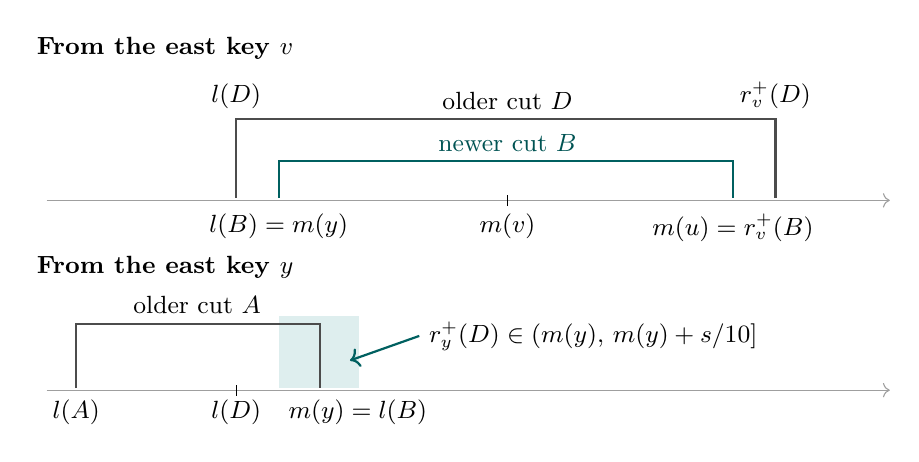
\begin{tikzpicture}[x=.83cm,y=.82cm,font=\small,
    axis/.style={->,gray!75},older/.style={draw=black!70,thick},
    newer/.style={draw=teal!75!black,thick}]
  \node[anchor=west,font=\small\bfseries] at (0,2.72) {From the east key \(v\)};
  \draw[axis] (.3,.36)--(13.2,.36);
  \draw[older] (3.2,.4)--(3.2,1.62)--(11.45,1.62)--(11.45,.4);
  \node[above] at (3.2,1.62) {\(l(D)\)};
  \node[above] at (7.35,1.62) {older cut \(D\)};
  \node[above] at (11.45,1.62) {\(r_v^+(D)\)};
  \draw[newer] (3.85,.4)--(3.85,.97)--(10.8,.97)--(10.8,.4);
  \node[above,text=teal!65!black] at (7.35,.97) {newer cut \(B\)};
  \draw (7.35,.27)--(7.35,.45);
  \node[below] at (3.85,.3) {\(l(B)=m(y)\)};
  \node[below] at (7.35,.3) {\(m(v)\)};
  \node[below] at (10.8,.3) {\(m(u)=r_v^+(B)\)};

  \node[anchor=west,font=\small\bfseries] at (0,-.68) {From the east key \(y\)};
  \draw[axis] (.3,-2.58)--(13.2,-2.58);
  \fill[teal!13] (3.85,-2.55) rectangle (5.08,-1.43);
  \draw[older] (.75,-2.55)--(.75,-1.55)--(4.48,-1.55)--(4.48,-2.55);
  \node[above] at (2.60,-1.55) {older cut \(A\)};
  \draw (3.2,-2.67)--(3.2,-2.5);
  \node[below] at (.75,-2.58) {\(l(A)\)};
  \node[below] at (3.2,-2.58) {\(l(D)\)};
  \node[below,anchor=north west] at (3.85,-2.58) {\(m(y)=l(B)\)};
  \node[anchor=west] (window) at (6,-1.74)
    {\(r_y^+(D)\in(m(y),\,m(y)+s/10]\)};
  \draw[newer,->] (window.west)--(4.94,-2.12);
\end{tikzpicture}
\caption{Transferring an endpoint. At \(v\), the first east charge
to \(B\) occurs at \(u\). Older cuts such as \(D\) set the scale bit
there. A west flag witness for \(B\) carries that same bit to \(y\).
At \(y\), the bit supplies a cut \(A\) with an old charge in the
shaded interval. Now \(D\) is newer than \(A\), forcing a mid charge
to \(D\) in that interval. Positions are schematic.}
\label{fig:cut-transfer}
\end{figure}

\begin{lemma}[Cuts charged by both spines]\label{lem:straddlers}
On the mid-color core list of depth \(f_*\) at any east key \(v\),
the cuts with \(r_v^+(B)<\infty\) have total weight at most \(t/a\).
\end{lemma}

\begin{proof}
Suppose the finite-endpoint cuts have weight greater than \(t/a\).
Starting at \(v\), we pass to another east key and retain a subfamily
of these cuts. Each step spends \(3H\) of depth and retains at least
\(a^{-4}\) of the weight. Every retained cut has a strictly smaller
finite right endpoint at the new key. This last property prevents
\(K\) such steps, since a cut has at most \(K\) keys.
Before each step we thus have \(f\ge9H\) and weight
\(M\ge t a^{-1-4(K-1)}\).

\emph{Selecting a nested pair.}
Group the cuts by the scale \(s\le r_v^+(B)-l(B)<as\), then by
the bins of width \(s/10\) containing their two endpoints. All these
intervals straddle \(m(v)\), so there are \(O_h(a^2)\) groups. One has
weight \(M'\ge c_h M/a^2\). Write \(\beta=t^2a^{-100K}\). The
bad ordered pairs in this group have product weight at most \(\beta\)
by Lemma~\ref{lem:good-comparisons}. Both orientations of a good
pair have the same product weight. Averaging, some cut \(B\) is
newer than cuts \(D\) of total weight at least
\((M'^2-\beta)/(2M')\ge M'/3\).

\emph{Reading the bit on the east.}
Let \(u\) be the east key at the first charge to \(B\) on the east
spine from \(v\). Every one of these older cuts \(D\) covers the
mid-color west test at \(u\) to depth \(f-H\), by
Lemma~\ref{lem:good-comparisons}. It therefore covers the old test
to depth \(4H\). Indeed each old path is allowed in the mid round,
and every mid charge on it is an old charge. By
Lemma~\ref{lem:proper-loss} applied between the list at \(v\) and the
old tests at \(u\), discard weight at most \(E_0\) to ensure
that no proper subset covers the old test at \(u\) to depth \(H_-\).
Since \(H_-<H\), this gives minimality at depth \(H\) as well. The
old and mid lists use the same requirement of possible screened
success for the keys of \(D\). Each remaining \(D\) therefore belongs
to the old core list at \(u\). Its former right endpoint occurs strictly
after \(u\) as an old charge on the continuing east spine. The common
right-endpoint bin and the choice of scale give
\eqref{eq:scale-bit}. The remaining mass exceeds \(\theta\).
Consequently the bit for \(s\) is set at \(u\), and the flag witness
for this charge to \(B\), which has east key \(u\), shows that the
bit is set in the given mid color.

\emph{Transporting the bit to the west.}
Take a mid west path at \(v\) witnessing the necessity, to depth
\(H\), of a west key of \(B\) at site \(l(B)\). At its first charge
to \(B\), go to the flag witness for this charge, and from the witness
move to its \emph{east} key \(y\). Thus \(m(y)=l(B)\). No older \(D\)
can have been charged before the first \(B\) charge, by the proof of
Lemma~\ref{lem:good-comparisons}. Going to the witness charges at most
the same west key of \(B\). For the move to \(y\), discard cuts
containing \(y\), of weight at most \(2p\) by
Lemma~\ref{lem:cut-list}. The prefix to \(y\) uses at most \(H+1\)
moves per site. Prepending it shows that the remaining \(D\)'s cover
mid west tests at \(y\) to depth \(f-3H\), and hence cover the old
tests there as well. By another application of
Lemma~\ref{lem:proper-loss} from \(v\) to \(y\), discard weight at most
\(E_0\) to ensure minimality to depth \(H\) in the old round. This
implies minimality in the mid round, since any covering subset in the
mid round covers the old tests. We have placed these cuts on the mid
core list at \(y\) of depth \(f-3H\) and the old one of depth \(4H\).

\emph{Forcing a new east endpoint.}
The witness at the west endpoint has the same mid color as the east
witness. Thus
the bit for \(s\) is set at its east key \(y\). At \(y\) the old list
contains cuts \(A\) of weight at least \(\theta\) charged at
\(x\le m(y)+s/10\) with \(l(A)\le m(y)-9s/10\).
By the product-weight bound on this old list, except for cuts \(D\)
of total weight at most \(\beta/\theta\), each transferred \(D\) has
a good comparison with such an \(A\). Since
\(\lvert l(D)-m(y)\rvert\le s/10\), \(l(D)>l(A)\).
Thus \(D\) has changed roles. At \(v\) it was older than \(B\).
At \(y\) it is newer than \(A\), so every key of \(D\) strictly
reaches the nearby key of \(A\).

The comparison at \(y\) was made in the old round. To finish the step
we need a \emph{mid} charge to \(D\) on the east spine from
\(y\) by site \(m(y)+s/10\). Otherwise follow the basic spine to
the east key \(g\) of the indicated old charge to \(A\).
That prefix misses \(D\) in the mid round. It uses at most three
moves per site, so \(D\) transfers to \(g\), covering even the old
west test to depth \(H\). Since \(g\in A\) and \((D,A)\) is good in
the old list, no proper subset of \(D\) covers that test even to
depth \(H_-\). Minimality forces \(g\) to reach every key of \(D\).
But every key of \(D\) strictly reaches \(g\) by the same comparison,
contradicting acyclicity.

The accumulated losses \(2E_0+2p+\beta/\theta\) are \(o(M')\),
and \(M'/3-o(M')\ge M/a^4\) for large \(a\). The new finite right
endpoint of every retained \(D\) is at most \(m(y)+s/10\), whereas
its former one was greater than \(r_v^+(B)\ge m(y)+s\). This proves
the asserted step. After \(K\) steps a retained cut would have had
\(K+1\) distinct right endpoints, each the site of one of its at most
\(K\) keys.
\end{proof}

\subsection{The direction and its barrier bits}

When the start moves east from \(v\) to \(u\), we transfer a west test
at \(u\) back to \(v\) by prepending the intervening spine. The
following depth vector saves four moves per visited site for exactly
that purpose. Define the \emph{band list} at an east key \(v\) to be
its mid-color core list with depth vector
\[
 F_v=f_*+(K+5)d+\sigma_v,\qquad
 \sigma_v(x)=
 \begin{cases}
 0& x<m(v),\\
 4& x=m(v),\\
 8& x>m(v).
 \end{cases}
\]
Compute the next refinement of a micro node at its east key \(v\).
If the total band weight is less than \(t/4\), append the symbol
\emph{neutral} and keep the west direction. Otherwise append the
unique \(b=(t/4)2^j\), \(j\ge0\), for which that weight lies in
\([b,2b)\), and set the direction east. In the latter case the gate
at this east key in this new color requires one additional bit for
each \(B\) on its band list. The bit is shared by all such gates
within the stage and new color that require it. Its index consists
of the stage, the new color, and \(B\). Choose its success
probability, depending only on the parameters, \(b\), and \(|B|\),
rationally in the interval
\[
 [\exp(-2\lambda r(B)/b),\,\exp(-\lambda r(B)/b)] .
\]
These are the only new barrier requirements. At any one key their
joint passage probability is at least \(\exp(-4\lambda)\). A new
gate requires the screened old gate, its fresh independent
key-thinning bit of probability \(z\), and the barriers just assigned.

Lemma~\ref{lem:cut-list} bounds every band weight by \(aU\), so there
are \(O(\log a)\) bins. With \(h\) fixed, the \(h\) scale bits and the
bins at each of the \(h-1\) refinement stages give polylogarithmically
many colors. The rules are local. A depth bound \(F\) gives a radius
at most \(L_0\max_x F(x)\), and minimality makes every cut key
reachable within such a bound. Coverage, possibility, and all
probabilities defining a screen can be evaluated from the resulting
finite unfoldings and the local rules of the preceding stages.

\subsection{The probability bound in the new direction}

We now relate the two deterministic lists used by the color rule to
the probability of coverage by successful gates. Three steps suffice.
Coverage after thinning usually produces a core cut of at most \(K\)
successful keys. Lemma~\ref{lem:two-spine-estimates} uses that cut to
bound the exceptional west tests. Proposition~\ref{prop:directional-cap}
then uses the shared barriers to obtain the cap after switching east.

Fix the mid color. Throughout, arbitrary sites may be ignored and
the raw bits there fixed arbitrarily. Count only hits at other sites.
Call a key \emph{thinned} here if its screened old gate and its new
thinning bit both succeed. Write \(f^\sharp=f+(K+4)d\), also for a
depth vector, with addition in each component.

\begin{lemma}[Extracting a cut after thinning]\label{lem:thinned-cover}
Let \(v\) be an east key and \(f\ge f_*\) a depth used in this stage.
Except on an event of probability \(o(t)\), mid west coverage at
\(v\) by thinned keys to depth \(f^\sharp\) implies that a cut on the
mid core list of depth \(f\) consists of nonignored thinned keys.
The error is uniform under the allowed conditioning.
\end{lemma}

\begin{proof}
Expose all bits through the preceding stage. Carry out the branching
search of Lemma~\ref{lem:cut-list} among the screened successes at
nonignored sites, stopping a branch when it covers to depth
\(f^\sharp-d\). Before it stops, any extension covering to depth
\(f^\sharp\) must use one of the \(a^{o(1)}\) candidates at its next
step. The candidates depend only on the exposed randomness. If
coverage by thinned keys occurs, follow only branches whose selected
keys survive thinning. Either one stops early or one reaches \(K\)
distinct surviving keys. Coverage also requires coverage in the crude
old test, an event of probability at most \(U\) measurable before
thinning. Thus the latter possibility together with coverage has
probability at most
\[
 Ua^{o(1)}z^K=o(t).
\]

On an early stopping branch the selected keys cover to depth
\(f^\sharp-d\). The minimum sizes of covering subsets of these keys
at depths \(f,f+d,\ldots,f+(K+2)d\) are nondecreasing integers in
\([1,K]\). Two consecutive values agree. A minimum subset at the
larger depth is minimal at the smaller, so belongs to the corresponding
two-depth mid list. If it fails to be minimal at depth \(H\), it has
a proper subset covering to \(H_-\). For each of the \(K+2\) possible
lists Lemma~\ref{lem:proper-loss} bounds the weight lost this way by
\(E_0\). A fixed cut of nonignored keys succeeds with probability at
most its weight, since it requires its independent pins. This adds
only \(O(KE_0)=o(t)\). Every remaining cut belongs to the claimed
core list.
\end{proof}

The two parts of the following lemma will bound coverage for the
neutral and switched colors, respectively.

\begin{lemma}[Coverage on the two spines]\label{lem:two-spine-estimates}
At every east key \(v\) the following estimates hold.
\begin{enumerate}
\item\label{item:small-band}
If \(v\) gives the neutral refinement, mid west coverage to
\((F_v)^\sharp\) by thinned keys has probability at most \(t/4+o(t)\).
\item\label{item:rare-joint-hit}
The probability of mid west coverage to \((f_*)^\sharp\) by thinned
keys \emph{and} a mid charge to a nonignored thinned key on the east
spine is \(o(t)\).
\end{enumerate}
\end{lemma}

\begin{proof}
The first estimate follows by the band weight and Lemma~\ref{lem:thinned-cover}.
For the second estimate, Lemma~\ref{lem:thinned-cover} provides a
successful cut \(B\) of depth \(f_*\), and Lemma~\ref{lem:straddlers}
costs at most \(t/a\) for cuts that meet the east spine. Otherwise
let the spine reach the charged thinned key \(g\). The screen at
\(g\) gives a missed old west path at depth \(d\) ignoring its site.
Prepend the east spine to \(g\). The concatenation is a mid west test
at \(v\) to depth \(f_*\), so must charge \(B\). All keys of \(B\) have
successful old gates. The hit must therefore be a key of \(B\) at
\(g\)'s site, distinct from \(g\). For fixed \(B\) there are at most
\(K\) candidate sites for \(g\) and at most one charged spine key at
each. At nonignored sites the additional pin is independent, so the
joint probability is at most \(Kp\,r(B)\). Summing gives at most
\(KpaU=o(t)\).
\end{proof}

\begin{proposition}[Coverage after one refinement stage]\label{prop:directional-cap}
For some \(D_i=O(D_{i-1}\log a)\), each new color has coverage
probability at most \(t\) in its chosen direction from every node
of its cluster, under arbitrary allowed conditioning on ignored sites.
\end{proposition}

\begin{proof}
For a neutral new color, test west from an arbitrary node. Follow its
west spine to the first charge in that color, go to its flag witness,
and from there to its east key \(v\), which gives the neutral
refinement. If there is no charge, coverage is impossible. The prefix
is deterministic, uses at most four moves per site, and has at most
two possible charges to nonignored keys in the new color. It has a
successful such charge with probability at most \(2p\). Otherwise
coverage at the starting node forces new west coverage at \(v\)
with the depth decreased by four, and hence mid west coverage there
by thinned keys. With starting depth at least
\(\max_x (F_v)^\sharp(x)+4\), Lemma~\ref{lem:two-spine-estimates}(\ref{item:small-band}) proves the
desired cap \(t\).

Consider finally a new color with bin \(b\), and an east key \(v\)
giving that refinement. Let \(\mathcal D\) be the intersection of the
band lists for the mid color over all east keys along the east spine
from \(v\), including \(v\). We claim
\begin{equation}\label{eq:common-bands}
 \sum_{B\in\mathcal D}r(B)\ge 0.9b .
\end{equation}
At \(v\) discard the cuts hit by that spine, of weight at most \(t/a\)
by Lemma~\ref{lem:straddlers}, since its band list is contained in
the core list at \(f_*\). For any later east key \(u\) on the spine,
prepend the spine prefix. It uses at most three moves per site, and
at each site used \(F_v(x)-F_u(x)\ge4\). Thus each retained cut
covers to \(F_u\) at \(u\). At the \emph{last} such east key discard
weight at most \(E_0\) by Lemma~\ref{lem:proper-loss} to guarantee
minimality to depth \(H_-\) there. From each earlier east key prepend
the segment to the last key to each witness of minimality. The segment
misses the cut and \(H_-+3\le H\), so this establishes minimality to
depth \(H\) at every one of them. A single application of the loss
bound therefore suffices to prove \eqref{eq:common-bands}.

By the good-pair averaging argument in Lemma~\ref{lem:straddlers},
applied now to the older member, there is \(D\in\mathcal D\) and
there are \(B\in\mathcal D\) newer than \(D\) of weight at least
\(b/4\). All of their corresponding barrier bits pass with probability
at most \(e^{-\lambda/4}\). A coverage test at \(g\in D\) uses only random bits indexed by
reachable keys or by sets of reachable keys. Every key of a newer
\(B\) strictly reaches \(g\), so acyclicity prevents \(g\) from
reaching any of them. The shared barrier bit indexed by \(B\)
is therefore independent of the coverage event at \(g\). This
independence also holds after the permitted conditioning on raw bits.

Suppose there is new east coverage at \(v\) to depth \(R>F_{\max}\),
where \(F_{\max}=f_*+(K+5)d+8\). The east spine must charge a successful
new gate. The charge has a flag witness of this new color with the
same east key. Hence that key assigns the bin \(b\) and requires
every shared barrier above. If thinned keys also cover the mid west
tests at \(v\) to depth \(F_v\), Lemma~\ref{lem:two-spine-estimates}(\ref{item:rare-joint-hit}) bounds this case by \(o(t)\), since
\(F_v\ge(f_*)^\sharp\) and the successful east charge is also a
thinned mid charge. Otherwise choose a missed mid west path to depth
\(F_v\). As \(D\) belongs to the band list, this path charges some
key \(g\in D\). Redirect this move to \(g\) itself. The prefix uses
allowed new moves, and every new charge is also a mid charge, so it
contains no nonignored successful new charge. It follows by
concatenation that new east coverage to depth \(R-F_{\max}\) must
hold at \(g\).

Let \(\Pi(R)\) be the supremum of new east coverage probabilities
over starting nodes in the cluster for this new color and the given
conditioning. From an arbitrary starting node use the east spine
up to its first new charge and go to its east key, which assigns
this bin by the flag witness. The prefix uses at most four moves per site. Its possible charged
keys are determined by the flags, before any random bits are read.
The probability of a nonignored success on the prefix is at most
\(2p\). Using the preceding implication at
that key, independence of the shared barriers, and a union bound
over the fixed set \(D\), we obtain
\[
 \Pi(R+4)\le o(t)+K e^{-\lambda/4}\Pi(R-F_{\max}).
\]
The coefficient \(\rho=K e^{-\lambda/4}\) is less than \(1/4\).
Start with the bound \(\Pi\le1\) and iterate
\(k=\lceil2J\log_2 a\rceil\) times. The contribution \(\rho^k\)
is at most \(a^{-4J}=t^4\), and the uniform errors sum to
\(o(t)/(1-\rho)=o(t)\). Thus \(\Pi\le t\) for large \(a\). A common depth \(D_i=O(D_{i-1}\log a)\) meets this
bound and the neutral one. Since \(h\) is fixed, every stage has
\(D_i=a^{o(1)}\). This completes the induction.
\end{proof}

\subsection{The last screen}

After stage \(h-1\), merge once more to the full interval. Set
\(d=D_{h-1}\). At depth \(d\) the crude cap \(U\) now applies to
coverage of all paths to leaves, since there are no exits. For each
key and color add a final screen forbidding this coverage with the
key's own site ignored. The resulting gate will be called final.

\begin{lemma}[A final gate and its continuation]\label{lem:final-gates}
For every key \(g\) and final color, its required raw bits have joint
success probability at least \(q^{-2}\), and its required barriers
have joint passage probability at least \(\exp(-4h\lambda)\).
Condition on the required raw successes at \(g\), optionally also
at one other key of the same site. The sum of the conditional
failure probabilities of its required screens is \(o(1)\), uniformly
over the allowed graphs and choices. Whenever the final gate at
\(g\) succeeds, there is a path from \(g\) to a leaf of per-site depth
at most \(d\) on which every charge to a successful final gate in
this color lies in the site of \(g\).
\end{lemma}

\begin{proof}
The raw probability is at least \(q^{-1}z^h=q^{-2}\). All barriers
ask for successes of deterministic sets of independent bits, so
multiplying their per-stage lower bounds gives the stated estimate.
For the screen of a given stage, later raw bits can be dropped from
the conditioning. Every subset of the remaining one or two pins is
in the key's site. The ignored-site crude cap gives conditional
coverage probability at most \(U\) under each such subset, so
Lemma~\ref{lem:pcost} gives conditional screen cost \(o(1)\).
The final screen costs at most \(U\) by the same crude cap. There
are at most \(h\) screens. Passage of the last one provides the
asserted path, since final successes are among the gate successes
tested by that screen.
\end{proof}

\section{One finite probability space for all layer lengths}\label{sec:finite}

Lemma~\ref{lem:final-gates} assigns random bits to keys and to sets of keys
in a directed acyclic graph. A term of Section~\ref{sec:numerical} can have
arbitrarily many distinct ancestors. Assigning a fresh bit to each ancestor
would make the probability space depend on the term. We instead index the
bits by finite descriptions of keys, called names. Two keys with the same
name receive the same bits. We choose the depth of the descriptions at
random. At each fixed key, with high probability the equalities between
names in its neighborhood are exactly the equalities of keys in some legal
graph. This local guarantee will suffice both for the occurrence probability
and for the path in Lemma~\ref{lem:primary}.

\subsection{Recognizing a legal neighborhood}

Fix the parameters of the gate construction. The \emph{unfolding} at a key
to radius \(R\) is the rooted tree of its move sequences of length at most
\(R\). A named unfolding records the node data, the available labeled move
slots and an equivalence relation on the occurrences, namely equality of
names. At each fixed depth there are only finitely many such patterns up
to renaming, since branching, slots and node data are bounded.

A color refinement is a function of a finite pattern from earlier rounds.
Give the function an arbitrary default on patterns where it was undefined,
proceeding through the rounds in order. Extend the local prescriptions of
raw, barrier and screen tests to all patterns in the same manner. These
extensions use only equality of names and preserve the bit indices on
realizable patterns.

\begin{lemma}[Local realizability]\label{lem:local-extension}
For every \(R\) there exists \(R'\ge R\) such that the radius-\(R\)
restriction of a named unfolding to radius \(R'\) is realized in the graph
model of Section~\ref{sec:probability} if it passes the following checks.
\begin{enumerate}
\item Equal names have the same node data. Whenever a move slot is
exposed at two occurrences of one name, it has the same target name.
\item The basic move rules and the prefix and witness rules for flags hold
wherever the neighborhoods needed to test them are exposed. In these
checks the colors are calculated by the extended refinement rules.
\item Identifying equal names in the graph of exposed moves creates no
directed cycle.
\end{enumerate}
\end{lemma}
\begin{proof}
If no such radius exists, there are counterexamples of arbitrarily large
radii. By successive extraction, stabilize their patterns at each finite
depth. In the limiting tree identify equivalent occurrences. The first
check makes each move well defined on the quotient. A directed cycle
would use finitely many exposed moves and name equalities, contradicting
the third check at a finite depth.

The second check gives the basic moves. Suppose the first rounds of
colors and flags already satisfy the rules of the graph model. These
rounds admit a legal completion by making all subsequent flags false.
The next refinement reads only the completed earlier rounds, so its
extended value is its specified value on the graph. The second check now
gives the prefix and witness conditions for the next flags. Induction
produces a legal graph, possibly infinite, whose root realizes the
stabilized radius-\(R\) pattern. This contradicts the choice of the
counterexamples.
\end{proof}

Put \(d=D_{h-1}\). Choose \(R\) large enough to evaluate the color
refinements and gate tests at the root, including the flags and gates at
charged keys along every path in the final screen. Such a path uses at
most \(dL_0\) moves. Fix the resulting \(R'\) from
Lemma~\ref{lem:local-extension}. A pattern passing its checks inherits
the probability bounds and the missed path of Lemma~\ref{lem:final-gates}.
Indeed, realization preserves every equality among the indices read by
these tests, so the local bits have precisely their graph-model joint law.

\subsection{Giving names to the keys of a term}

The two blank layers of each site are its shores. A nonleaf blank term has
its two parent steps as basic moves. Attach two temporary blank leaves to
each micro leaf, one on each shore of its site. From a micro term, a
straight run of parent steps in either direction now reaches a first blank
term, its direction key. Compress this straight run, or \emph{leg}, into
one basic move to its key. A witness jump in the same direction will end
at a strictly older micro term on the leg, with the same direction key.
When we return to the original terms we stop a path at the micro leaf
preceding a temporary blank.

Choose a radius \(j\) uniformly among the integers
\(N_*,\ldots,2N_*-1\). In round zero this range is a single bin. In each
later round subdivide every preceding bin into equally many consecutive
bins of equal size. We first choose the subdivision counts, then take
\(N_*\) sufficiently large and divisible by the number of final bins.
Each bin in a round has its own flags and witness slots.

To define names, retain the moves and flags for \emph{all} bins, the site,
the node type and an auxiliary symbol. The \(j\)-name of a term is the
tree of its moves truncated after \(j\) levels, with these data through
depth \(j\). It records neither identities of terms nor the positions of
micro layers within a site. Once the parameters and subdivision counts
are fixed, the number of outgoing move slots is bounded. Choose a finite
ordered alphabet larger than the number of strict ancestors that can be
reached in \(2N_*\) enriched moves. Each term takes the first symbol
absent at those ancestors. The symbol is part of its name, but the local
rules use names only for equality. In particular, the check radius
\(R'\) was fixed before choosing the auxiliary alphabet.

Process terms in order of construction, with temporary blanks first and
parents before their merges.
\begin{itemize}
\item A blank term has known outgoing moves. Assign its symbol, form
its names and compute every round's refinement outputs for every \(j\).
Use equality of \(j\)-names and the bins containing \(j\) in the
previous rounds. Call a round's bin \emph{stable at the key} if the vector
of outputs for all input colors is constant on that bin. Round zero is
stable.
\item In a bin a micro term is \emph{live} if both direction keys are
stable in that bin and in every containing bin of earlier rounds. Its
calculated color is then constant on the bin. On each leg set flags for
exactly the colors of the live micro terms encountered, including the
source. Witness each flag by the first such occurrence of its color.
If the source is the witness, no jump is needed. Otherwise the
corresponding slot jumps to the witness. Assign the source its auxiliary
symbol after all these moves have been determined.
\end{itemize}
In the second step the source's liveness and color are calculated from
its two keys, both strictly older, so the specification is recursive.
Every witness keeps the same direction key along the leg. Its liveness
in the preceding bin supplies the flag for its prefix color.

\begin{lemma}[Finite names]\label{lem:finite-names}
Given \(\varepsilon>0\), the subdivisions and \(N_*\) can be chosen
independently of the numbers of micro layers so that, for each fixed blank
term, with probability at least \(1-\varepsilon\) over \(j\),
\begin{enumerate}
\item the bin containing \(j\) is stable at this key in every round, and
\item the unfolding at this key computed with the bins of \(j\) and
equality of \(j\)-names passes the radius-\(R'\) checks of
Lemma~\ref{lem:local-extension}.
\end{enumerate}
\end{lemma}
\begin{proof}
Inside a bin of the preceding round, the flags and move slots read by the
current refinement are fixed. It inspects at most \(u\) occurrences. Here
\(u\) may be chosen uniformly for the fixed local rules, since the
refinement reads one bin per earlier round. Increasing \(j\) only refines
the partition of these occurrences by name equality. Each strict
refinement adds at least one class. Between refinements the output vector
is constant, so at most \(u-1\) of the new bins can be unstable. Choose
enough bins at each subdivision that, summed over the finitely many
rounds, the probability of instability is less than \(\varepsilon/2\).

With these counts fixed, the radius-\(R'\) tree using the slots of
\emph{all} bins contains at most \(M\) occurrences, independently of
\(N_*\) and the lengths of the sites. Its partition by \(j\)-names
can strictly refine at most \(M-1\) times between depths \(j\) and
\(j+1\). For every other \(j\), equal \(j\)-names among these occurrences
have identical \((j+1)\)-names and hence, in every exposed slot, targets
with identical \(j\)-names. This gives the first check. The decoration
gives the second, since each witness is evaluated with the same bin and
the same name equalities that supplied its flag.

For the third check, suppose the identified graph has a simple directed
cycle of length \(m\le M\). Follow the cycle's slots in the actual tree
starting at its first representative. After one step the subtree agrees
with the next representative to depth at least \(j-1\): the chosen slot
occurs in the starting name and its target has the next representative's
name. At each succeeding step at most one more level of agreement is
lost. If \(N_*>M\), the terminal term agrees with the starting one at
least through depth zero. It therefore has the same auxiliary symbol,
although it is a strict ancestor within \(m\le 2N_*\) enriched moves.
The choice of symbols excludes this. Finally choose \(N_*\) so large
that \((M-1)/N_*<\varepsilon/2\). This bounds the probability of failure
of the checks and completes the proof.
\end{proof}

\begin{proof}[Proof of the Primary Lemma (Lemma~\ref{lem:primary})]
Call a blank key \emph{good} at \(j\) when both conclusions of
Lemma~\ref{lem:finite-names} hold there, with
\(\varepsilon=L_0^{-10}\). An outcome selects \(j\), a uniform final color,
and a common table of independent gate bits, independently of one another.
Supply entries for every syntactically possible index of a raw or barrier
bit. Replace keys by names and sets of keys by sets of names, and retain
the prescribed stages, colors, and other index data, including the sizes
of sets when these affect a bit's law. The screens read this same table.
All trees naming the bits have bounded depth over a finite alphabet.
Hence the outcome space \(\Omega\) is finite and works for every choice
of the numbers of micro layers.

For a micro term \(v\) let \(P(v)\) consist of the outcomes for which
both direction keys are good, the term has the selected final color,
and both keys' final gates succeed in that color. For a blank term put
\(P(v)=\varnothing\).

The two keys of \(v\) are good together with probability at least
\(1-2L_0^{-10}\). Fix such a radius. Conditional on selecting the color
of \(v\), their joint raw successes have probability at least \(q^{-4}\)
by Lemma~\ref{lem:final-gates}, since their opposite shores distinguish
their names. Condition on these successes. At each key the sum of the
conditional failure probabilities of its screens is \(o(1)\). To see
why the conditioning at the other key is allowed, if its name occurs
in the local test, it denotes a key of the same site in the realizing
graph. If its name is absent, its raw bits are independent of that test.

At each key the required barrier bits pass with probability at least
\(\exp(-4h\lambda)\). Shared barrier bits require the same success, so
the probability that both prescriptions pass is at least
\(\exp(-8h\lambda)\). These bits are independent of the raw bits.
Subtracting the sum of the conditional screen failure probabilities
therefore gives, with \(k_f=a^{o(1)}\) final colors,
\[
 \Pr(P(v))\ \ge\ (1-2L_0^{-10})\,k_f^{-1}q^{-4}
       \bigl(\exp(-8h\lambda)-o(1)\bigr)\ \ge\ q^{-5}.
\]
The last inequality holds for sufficiently large \(a\), since \(q=a^w\)
and \(h,\lambda,w\) depend only on \(C\). The allowed powers of two \(a\)
in~\eqref{eq:prob-parameters} give arbitrarily large powers of two \(q\).

Fix an outcome and a starting blank term in site \(s\). Say a charge
succeeds if its key is good and its final gate succeeds in the selected
color. Expand each compressed move to its straight sequence of parent
steps. A potential occurrence on this sequence, with the source included
and the destination excluded, forces a successful charge at that move.
Indeed, such an occurrence is a live micro term of the selected color
on the source's leg, and the common direction key is good with
a successful gate. The color at that occurrence sets the source's flag.
The half-open convention includes a micro leaf whose move ends at a
temporary blank.

Follow the basic spine pointing out of \(s\). If no charge succeeds, it
ends at a leaf without an occurrence. Otherwise its first successful
charge takes the basic move to its key in a site \(s'\ne s\). Its
expansion so far can have occurrences only on this last leg, which lies
in \(s'\). At this good key local realizability and Lemma~\ref{lem:final-gates}
supply a continuation to a leaf on which all charges to successful final
gates of the selected color belong to \(s'\). The path lifts by following
its labeled slots in the actual term. Our choice of \(R\) includes every
move of the path and every gate test at its charged keys. Thus every
potential occurrence on its expanded path belongs to that site.
The two pieces use at most \(3L_0\) and \(dL_0\) compressed moves
respectively. Each expands in a single direction, so the path has at
most \((d+3)L_0\) turns. Stop at the original leaf before any temporary
blank. This gives the path and the uniform turn bound of
Lemma~\ref{lem:primary}.
\end{proof}

\section{Realizing the scheduler by blocking inequalities}\label{sec:layers}

At a probe for bucket \(P\), the scheduler of
Theorem~\ref{thm:scheduler} must make enough of the corresponding red
rows tight to serve the client program. Each red row will be a lower
bound on an affine expression, called an \emph{output}. A module has two
ways to supply a tight output. It can attain one of its own bounds, or
it can transmit tight bounds from all of its children at one label.
Section~\ref{sec:vertex} proves this alternative for the inequalities
constructed here. Section~\ref{sec:compiler} chooses modules to match
the alternative to the options in the client program.

\paragraph{One episode.}
Write \(x_P\) for the probe of bucket \(P\) in a single episode.
One coordinate \(v_P\) per bucket suffices to realize the first alternative
at height zero. Impose
\begin{equation}\label{eq:base-module}
 v_P\ge0,\qquad v_P+v_{P'}\ge1\quad(P\ne P'),\qquad
 v_P\ge I_0|x-x_P|-1 .
\end{equation}
Choose \(I_0\) so that the time-dependent bound for \(P\) is at
least two at every other probe and at both anchors. At \(x_P\) its
value is \(-1\), while each retained \(v_{P'}\) for \(P'\ne P\) is at
least two. Thus \(v_P\) can move in both directions if it is present
and positive. At a vertex that retains it, the floor \(v_P=0\) must
be tight. Reusing a coordinate at two separated probes poses a new
problem. A convex lower bound low at those probes stays low between
them. The numerical construction provides many different zero sets
on the same coordinates. They will distinguish the sites in a time
block, while the prices introduced below select children to serve at
a probe.

\subsection{From ordered layers to prescribed times}

Fix \(r\ge100\). The positions \(\mathcal A\) will carry a tournament
in which each set of at most \(2^r\) positions has a common dominator
outside the set. Such a tournament exists. For a fixed \(j\)-set in
a uniform random tournament on \(a_0\) positions, with \(1\le j\le
2^r\), the probability of having no common dominator is
\((1-2^{-j})^{a_0-j}\). Multiplying by \(\binom{a_0}{j}\) and summing
over these \(j\) gives a bound tending to zero as \(a_0\to\infty\).
Fix the tournament once for this \(r\).

Apply Theorem~\ref{thm:coarse} with \(C=1000r^2\). Choose a power of
two \(q\) supplied by that theorem and take \(L=(q^C)^k\) for sufficiently
large \(k\). Its field size \(b\), the least power of two at least
\(L^{1/(r+1)}\), then accommodates all the positions. Every block
will use the same label alphabet
\[
   \mathcal I\times\mathcal A\times\mathbb F_b,\qquad
   H_i(s)=\{(i,a,\mathrm h_a(s)):a\in\mathcal A\}
    \quad(i\in\mathcal I,\ 1\le s\le L).
\]
Here \(H_i(s)\) is the bundle assigned to site \(s\) by index \(i\).
Since \(\lvert\mathcal I\rvert\le L^{8/C}\), the total number \(V\)
of labels satisfies
\[
 V\le 2|\mathcal A| L^{8/C+1/(r+1)},\qquad 10V\le L^{3/r}
\]
for all sufficiently large \(k\).

At each site the theorem allows a blank sample, any positive number of
interior samples, and another blank sample. At an interior sample of
site \(s\), every state vanishes on some whole \(H_i(s)\) and has at
most \(r\) zeros on any bundle of a different site. Its third conclusion
bounds the number of states at a sample independently of the number of
interior samples. We now use its merge inequality to realize these
states at the \emph{prescribed real times}, including unevenly spaced ones.

For a sample time \(x\) with immediate neighbors \(x^-<x<x^+\), write
\(x=\alpha_x x^-+(1-\alpha_x)x^+\). Choose a single positive integer
\(e\) for the finite sequence so that \(4^{-e}<\min(\alpha_x,1-\alpha_x)\)
at every such \(x\). Raise each entry of every state to the power \(e\).
The zero sets persist and the merge factor in
Equation~\eqref{eq:layermerge} becomes \(4^{-e}\). Let \(Z_x\) be the
convex hull of the powered states at \(x\) plus the nonnegative
orthant. For \(c\ge0\), the value
\(m_c(x)=\min\{c\cdot v:v\in Z_x\}\) is attained by a powered state.
Merging minimizing states at the two neighbors gives
\[
 m_c(x)\le 4^{-e}\bigl(m_c(x^-)+m_c(x^+)\bigr)
        \le \alpha_x m_c(x^-)+(1-\alpha_x)m_c(x^+).
\]
The last inequality is strict whenever \(m_c(x)>0\), since the two
neighboring values then have positive sum. Thus the linear interpolation
of the data \(m_c\) is convex and bends strictly at each interior time
where the data are positive. At any sample \(x_0\) with \(m_c(x_0)>0\),
choose an affine function \(b_c\) equal to \(m_c\) there and strictly
below it at every other sample. At an interior sample one may use any
slope strictly between the two chord slopes. At the first or last
sample use a slope below or above its adjacent chord slope, respectively.

\subsection{Time blocks and the forest of modules}
Time blocks organize the sample times. Modules organize the physical
coordinates. Blocks at one height are disjoint intervals of time,
and the same module serves all of them.

Arrange the $N=L^h$ episodes as the leaves of an ordered $L$-ary
tree of time blocks. A block of height zero contains the anchors
and probes of one episode. A block $E$ of positive height has one
site $s$ for each of its children $E_s$. All samples of $E_s$,
including its own blanks if any, are interior samples of that site.
Insert two new blank samples around them. The gaps between prescribed
episodes leave room for all internal insertions, and the outermost
blanks can be placed beyond the episodes. Every prescribed probe is an
interior sample of its site at each positive height, so the zero-bundle
conclusion applies there. The added blanks serve only the interpolation
within the block that inserted them. A common exponent \(e\) can be chosen
for the finitely many interpolation triples in all the blocks. The
total number of distinct times, including the new blanks, is
$S=O(NB)$, since two blanks are added per tree edge. Whenever sample
data on the whole tree are interpolated, we use linear interpolation in
their order and extend the two outermost pieces affinely to the line.

A separate finite forest specifies which coordinates we use. Each
module owns distinct coordinates. The roots are
modules of height $h$. A module of height $t>0$ may have any number of
children of height $t-1$ at each label, and modules of height zero
have no children. Its own outputs, called quick outputs, come in classes with one member
per bucket $P\in\{1,\ldots,B\}$. It also propagates each output class
of each child as a separate class of its own. Thus a root has one
class for each quick-output class in its subtree. The rows bounding
these root outputs below will be the red rows. At any fixed time the
root systems use disjoint coordinates, so their joint slice is a product.

All modules use one physical time $x$. Each module has a fixed set of
physical coordinates shared across its blocks. To state the inequalities
for block $E$, take the local value of every output to be its physical
value minus
\begin{equation}\label{eq:module-shift}
 D_E(x)=T_E(x)+R_t(x),
\end{equation}
where $T_E$ is affine and $R_t$ is convex piecewise affine, common
to all blocks of this height. At height $h$ we set the shift to zero.
At the samples in \(E\), its lines and shifts will make the local system
of this block govern its module. We first give those local inequalities.

At height zero there is one physical coordinate per bucket. Subtracting
the shift \eqref{eq:module-shift} gives the local coordinates $v_P$ in
\eqref{eq:base-module}. Choose a common $I_0$ large enough to serve all
height-zero blocks.

\subsection{Local inequalities at positive height}
Fix $t>0$ and a block $E$ of height $t$.
The child systems are already fixed. Their pair bounds have positive
gaps, and Lemma~\ref{lem:descent} at height \(t-1\) supplies an allowance
for raising their local output floors independently at probes. Choose
\(\delta>0\) with \(10\delta\) smaller than all those gaps and with
\(2\delta\) within the child floor allowance. In assigning the shifts
at height \(t-1\), take \(0\le R_{t-1}\le\delta/8\) at all samples.
The final paragraph describes the choices in inductive order.

At each label $\ell$ introduce local variables $W_\ell,p_\ell$ and,
for every bucket $P$, quick outputs $F_{\ell,P},G_{\ell,P}$. The
$F$'s at a fixed label constitute one class, and the $G$'s another.
If a child attached at $\ell$ has physical output $v_j^{\rm phys}$,
its propagated output in this block is the expression
\begin{equation}\label{eq:module-propagation}
 Y_j=p_\ell+\varepsilon v_j^{\rm phys}.
\end{equation}
The index $j$ includes the child identity. No new coordinate is
introduced for $Y_j$. Take $\mu=\sigma^2$ and $\varepsilon=\sigma^3$,
where $\sigma>0$ will be chosen small at this height. Impose output
floors $F,G,Y\ge0$. A floor raise in a fixed slice refers to an
increase of one of these local lower bounds.

\paragraph{Numerical constraints.}
Use the states and $Z_x$ for this block, and require $W\ge0$.
Choose a piecewise affine function $g$ with positive values at
all samples, so that adding any offsets in $\{0,1\}$ to its sample
values still gives concave data. A sufficiently large multiple of
$-x^2$ on the finite sample set, translated upward and interpolated,
has this property. We use the same \(g\) on the full sample set at this
height. Write $z=W-\sigma g(x)\mathbf1$ and let $z^+,z^-$
denote its positive and negative parts, both taken nonnegative.
The numerical rows must reproduce the following condition at each
sample \(x\) of \(E\):
\begin{equation}\label{eq:layer-state}
 z^+\in D Z_x,\qquad D=1+M_0\sum_\ell z_\ell^- .
\end{equation}
A coordinate of \(W\) is allowed to fall below the offset
\(\sigma g(x)\). When that happens the negative parts of \(z\) enlarge
the required positive part by the factor \(D\). The following rows
implement this compensation with nonnegative coefficients.

Apart from nonnegativity, $Z_{x_0}$ is described by its facet
inequalities $c\cdot v\ge m$, with $c\ge0$ and $m=m_c(x_0)>0$.
Indeed its recession cone is the nonnegative orthant, and an
inequality with minimum zero already follows from $v\ge0$.
The number of facets is bounded in the fixed parameters, since each
face is generated by a subset of the boundedly many states and coordinate
rays. For all the finitely many facets and samples in use take $M_0$
large enough that $M_0m\ge\max_\ell c_\ell$. If $b_c$ is the affine
minorant of $m_c$ touching only at $x_0$, impose
\begin{equation}\label{eq:coarse-rows}
 c'\cdot W\ge b_c(x)+\sigma\|c'\|_1g(x_0)
\end{equation}
for each $c'$ formed by replacing any subset of the entries of $c$
by $M_0m$. At $x_0$ the least value of $c'\cdot z$ over these
choices is $c\cdot z^+-M_0m\sum_\ell z_\ell^-$. Hence the rows
generated there enforce exactly \eqref{eq:layer-state}. At any other
sample $x$ of $E$, its own rows suffice. Since $W\ge z^+$ and $c'\ge c$,
we have $c'\cdot W\ge m_c(x)$ by \eqref{eq:layer-state} and the
inclusion $D Z_x\subseteq Z_x$ for $D\ge1$. The strict gap
$m_c(x)-b_c(x)$ makes \eqref{eq:coarse-rows} strict there for small
enough $\sigma$.

\paragraph{Links and prices.}
Let $o_P$ have value one at probes for $P$ and zero at every other
sample. At such a probe the quick outputs in $P$ will be called
\emph{target outputs}, and those in the remaining buckets \emph{other-bucket outputs}. Impose
\begin{equation}\label{eq:module-link}
 F_{\ell,P}\ge W_\ell-\sigma (g+o_P)(x),\qquad
 p_\ell\ge W_\ell-\sigma g(x)-3\mu .
\end{equation}
At the target probe the first link allows one extra \(\sigma\) of slack.
In Lemma~\ref{lem:descent}, this slack frees the price from its link to
\(W\) at a zero coordinate of the limiting state. A tournament on each
bundle will select one of the freed prices for the common descent. Enforce $p_\ell\ge-K_0\varepsilon$, with $K_0$ so large
that $K_0-T_{E_s}(x)-\delta>0$ for all relevant sites and samples.
For every site $s$ set
\[
 u_\ell^s=-p_\ell/\varepsilon-T_{E_s}(x)-\delta .
\]
Thus \(u_\ell^s\) measures the price in the units of a child at site
\(s\), with sign reversed. The price floor gives a common upper bound
\(K_1>0\) for these quantities at the samples. Choose $M_1>1$ such that $rK_1/M_1<\delta/2$.
For every $H_i(s)$ and every list $\ell_0,\ldots,\ell_r$ in it whose
positions form a transitive tournament in the stated order (each
beats all later positions), impose
\begin{equation}\label{eq:module-tournament}
 \sum_{j=0}^r M_1^{r-j}u_{\ell_j}^s\le0 .
\end{equation}

For the link to the second quick output put
$\mathcal D(x)=\max_{E'}D_{E'}(x)$ over all blocks of height $t-1$.
Take $0<\lambda<\delta/4$ so small that the sample values of
$\mathcal D+\lambda-2\lambda o_P$ are convex for every $P$.
This is possible because $\mathcal D=R_{t-1}+\max T_{E'}$ has strict
bends in its sample data. With the expression in parentheses
interpolated from those values, impose
\begin{equation}\label{eq:module-g}
 G_{\ell,P}\ge p_\ell+\varepsilon
       (\mathcal D+\lambda-2\lambda o_P)(x).
\end{equation}
Finally give each pair of distinct outputs within a class a positive
gap. For their sum the lower bound is
\begin{equation}\label{eq:module-pairs}
 \mu\quad\text{in an $F$ class},\qquad
 \varepsilon\lambda/4\quad\text{in a $G$ class},\qquad
 \varepsilon\delta\quad\text{in a propagated class}.
\end{equation}

\subsection{One blocking system for all blocks}
At positive height the actual coordinates of a module are
\begin{equation}\label{eq:module-coordinates}
 W_\ell^{\rm phys},\quad p_\ell^{\rm phys}-W_\ell^{\rm phys},\quad
 F_{\ell,P}^{\rm phys}-W_\ell^{\rm phys},\quad
 G_{\ell,P}^{\rm phys}-p_\ell^{\rm phys}.
\end{equation}
We refer to these, in order, as the coordinates associated to $W,p,F,G$.
For block $E$, subtract $D_E$ from the physical variables $p,F,G$ and
$D_E/2$ from $W$ to obtain local variables. Descendant variables in
\eqref{eq:module-propagation} keep their physical values. This makes
the physical propagated output $p_\ell^{\rm phys}+\varepsilon
v_j^{\rm phys}$, with the same shift as a quick output.

This choice of coordinates separates the differences in the links from
the sums in output floors. For example, \(p_\ell^{\rm phys}\) is the sum
of the first two coordinates, and \(G_{\ell,P}^{\rm phys}\) is their sum
plus the fourth. Propagation adds a positive multiple of a descendant
output. Thus each output is a nonnegative linear combination of blocking
coordinates. We verify the convexity of the corresponding time bounds.
In particular, \eqref{eq:module-link} and \eqref{eq:module-g} bound single
difference coordinates. The former acquires the convex shift $D_E/2$
and the latter has zero shift. The negative interpolants of \(g\) and
\(g+o_P\) are convex, as is the interpolant in the \(G\) link. The numerical rows acquire nonnegative
multiples of $D_E$. Equation~\eqref{eq:module-tournament} bounds a
positive weighted sum of physical prices below by an affine function
plus a positive multiple of $D_E$. Output floors and pair rows also
acquire nonnegative multiples of $D_E$. Each such lower bound
represents the finite list of its affine pieces, all imposed on the
whole time line. Even after removing every output floor, a bound on
each single coordinate remains, from $W\ge0$ and the links, or from
the absolute-value bound at height zero.

Choose the lines $T_E$ at each height with slopes increasing in the
order of the blocks and with successive intersections lying in the
gaps between them. Then $T_E$ is the unique highest line at every
sample of $E$. Scaling all these lines by a common positive factor
makes the gaps between the highest line and the others arbitrarily
large at those finitely many samples. In particular
$\mathcal D(x)=D_{E_s}(x)$ at the samples of $E_s$.
We check that the current block imposes all the required inequalities
at its samples. Express a feasible point for $E$ in the local variables of
another block $E'$. The values of $F,G,p$ and all propagated outputs
increase by $D_E-D_{E'}$, and $W$ increases by half that amount.
The difference $G_{\ell,P}-p_\ell$ is invariant under this change,
and its lower bound in \eqref{eq:module-g} is shared by all blocks at
height $t$. Thus the copies of this link in $E$ and $E'$ have exactly
the same slack, which may be zero. For each remaining row of $E'$
the left side gains a positive multiple of $D_E-D_{E'}$. Before this
gain its value is bounded below uniformly on the current slice.
Use the floors and links for individual quantities and differences,
$W\ge0$ for numerical rows, and the price floors for the tournament.
There are finitely many rows and samples. One scaling therefore gives
strict slack in every off-block row other than the shared links.
At height zero every off-block row gains positive slack by the same
argument. Raising current output floors preserves the implications. The conclusion also holds after coordinate restriction. The system of
\(E\) and its descendants has nonnegative coordinate normals, so any
feasible restricted point can be lifted by taking omitted coordinates
sufficiently large. The full lift satisfies the other blocks' rows,
and hence so does its projection for every such row that is retained.

The construction in height is inductive. First fix all times,
numerical states, and powers. Construct the local systems at height
zero. Their pair gaps and allowable raises of the output floors
determine how small the next $\delta$ must be. After each height
$t<h$ has acquired its local pair gaps and positive floor allowance,
choose the next $\delta$ accordingly, then choose $R_t$ by interpolating
a sufficiently small positive multiple of $x^2$ on the full sample
set, so that $0\le R_t\le\delta/8$ there. Choose the lines $T_E$ at
that height as above. Thus when the next height is constructed all
child shifts are fixed. At a positive height first choose
$g,M_0,K_0,K_1,M_1,\lambda$, then choose a common sufficiently small
$\sigma$ for all its modules and blocks. Lemma~\ref{lem:descent}
gives a uniform floor allowance in these local systems, using only
their probe slices and the already fixed child systems. Thus its
choice of $\sigma$ and allowance is independent of the current
height's shifts. At the root height there is one
block, its shift is zero, and its output floors are single affine rows.

\section{A tight output or a descent at a probe}\label{sec:vertex}

The output floors transmit information down a subtree and back to
its root. Fix a probe \(x\) for bucket \(P\), and at each module use
the local coordinates of the block containing \(x\). Under a coordinate
restriction, a floor is \emph{retained} when its row is supported on
the retained coordinates. At the current module one may raise each
retained output floor independently from zero to a prescribed value.
This includes floors on propagated outputs. The descendant systems
initially keep their original inequalities.

Call a module \emph{ready} if the restriction keeps its coordinates
associated to \(W_\ell,p_\ell,F_{\ell,P},G_{\ell,P}\) for every label
\(\ell\). At height zero it suffices to keep the output coordinate for
\(P\). Readiness is a condition on this one module.

\begin{lemma}[Descent at a probe]\label{lem:descent}
The parameters at each height can be chosen with a positive allowance
for independent raises of the module's output floors. For every choice
of raises within that allowance, each vertex of the restricted slice
of a ready subtree has at least one of the following properties.
\begin{enumerate}
\item A quick output of the module in bucket $P$ is at its floor.
\item The module has positive height and has a label $\ell$ with the
following property for every child at $\ell$. After allowed raises of
that child's output floors, the point restricted to its subtree is a
vertex. A retained child output is at its prescribed floor precisely
when its propagated output is at its floor in the parent.
\end{enumerate}
The second alternative includes a label with no children.
\end{lemma}

The two quick outputs in bucket \(P\) enforce this alternative in
different ways. If neither kind is tight, we first find a bundle of
labels on which the link between \(W\) and the price \(p\) is slack.
The \(F\)-outputs are responsible for this freedom. The tournament
then singles out a label in the bundle, and a \(G\)-output forces its
price into the interval in which the parent floors become admissible
raises in every child.

\begin{proof}
At height zero take allowance $1/2$. At the probe for $P$, the
absolute-value bound on its output has value $-1$, and every other
present output is at least $2$. All pair bounds touching the $P$
output are therefore strict. Unless that output is at its floor, it
can move in both directions.

For a module of positive height we prove that \(\varepsilon\lambda/4\)
is an allowance. The child systems and their shifts are already fixed.
Suppose there are arbitrarily small \(\sigma>0\) for which the
assertion fails. Take a sequence \(\sigma\downarrow0\) and, for each
term, a counterexample vertex with prescribed raises
\(0\le a_j\le\varepsilon\lambda/4\). Pass to a subsequence fixing the
module, probe and coordinate restriction. In particular, every
retained target quick output is strictly above its prescribed floor.

At this sample we need only the current block's rows at the module
(Section~\ref{sec:layers}). By readiness the triangular change
\eqref{eq:module-coordinates} is invertible on the retained variables.
All prices and target outputs are present. An output from another
bucket is used only when its associated coordinate is retained.

\smallskip
\noindent\emph{Bounds for the children.}
Keep the current module fixed. Each child point is then a vertex of its
own restricted system augmented by the propagated floors and pair rows
from the parent. The frozen section is a product
over children, since a pair of propagated outputs belongs to a single
class from a single child. Dividing these extra rows by $\varepsilon$
gives fixed normals and right-hand sides $a_j/\varepsilon-p_\ell/\varepsilon$
and $\delta-2p_\ell/\varepsilon$, respectively. The price floor
$p_\ell\ge-K_0\varepsilon$ and the bound $a_j\le\varepsilon\lambda/4$
bound these right-hand sides above. For a tight extra row its right-hand
side also has a lower bound. Indeed it then equals the corresponding
physical child output or the sum of two such outputs, and a retained
parent row includes the supports of the relevant child floors. Indeed
the output expressions have nonnegative coefficients in the coordinates
\eqref{eq:module-coordinates}, so their supports cannot cancel in a sum.
The child floors give fixed lower bounds at \(x\). A vertex is determined by
linearly independent tight rows of full rank in the retained child
coordinates. Their normals come from finitely many fixed matrices, and
all their tight right-hand sides have just been bounded on both sides.
Thus the child coordinates remain bounded as \(\sigma\downarrow0\).

\smallskip
\noindent\emph{A common limiting state.}
Now freeze the children instead. The current node is a vertex of this
section. Recall from \eqref{eq:layer-state} that $z=W-\sigma g(x)\mathbf 1$
and that its coarse constraint is $z^+\in D Z_x$, with
$D=1+M_0\sum_\ell z_\ell^-$. Hold this particular value of $D$ fixed
and replace $W$ and all its constraints by
\[
  \widehat z\in D Z_x,\qquad
  F_{\ell,Q}\ge\widehat z_\ell-\sigma o_Q(x),\qquad
  p_\ell\ge\widehat z_\ell-3\mu .
\]
The point with $\widehat z=z^+$ is feasible. At negative entries of
$z$, the displayed output links follow from $F_{\ell,Q}\ge0$ and
$p_\ell\ge-K_0\varepsilon>-3\mu$ for small $\sigma$.
It is still a vertex. Any two-sided motion in the new section fixes
the zero entries of $\widehat z$ by nonnegativity. Restore their
original $z$-values and let the other entries move with $\widehat z$
on a sufficiently short segment. All negative parts stay fixed, so the
original dilation is preserved. The original links follow from
$z\le\widehat z$, and $W\ge0$ holds since moving entries of $z$
are positive. This would lift any nonzero two-sided motion to the
original section.

Divide the current variables by \(D\), writing dots for the
result. Since \(W\ge0\),
\[
        1\le D\le 1+M_0V\sigma g(x).
\]
In the divided coordinates every constraint can be written with a
normal independent of \(\sigma\). For the tournament constraints,
first multiply \eqref{eq:module-tournament} by \(\varepsilon\).
The frozen child coordinates are bounded, so propagated floors and
pair rows give lower bounds on \(\dot p_\ell\) of order
\(O(\varepsilon)\). The limiting inequalities reduce to
\[
 \dot{\widehat z}\in Z_x,\qquad
 \dot p_\ell\ge\dot{\widehat z}_\ell,\qquad
 \dot F_{\ell,Q}\ge\dot{\widehat z}_\ell,\qquad
 \dot G_{\ell,Q}\ge\dot p_\ell .
\]
All remaining rows follow from these inequalities. Their right-hand
sides tend to zero, and their left-hand sides are nonnegative
combinations of the displayed variables. Take a further subsequence
on which one nonsingular matrix of tight rows determines the divided
vertex. Its right-hand sides converge, so its solution converges and
the same independent rows remain tight in the limit. The limit is
therefore a vertex of the displayed polyhedron. The differences
$\dot p-\dot{\widehat z}$, $\dot F-\dot{\widehat z}$ and $\dot G-\dot p$,
taken label by label, identify the limiting system
with $Z_x$ times an orthant. At a vertex all those differences vanish and
$\dot{\widehat z}$ equals a vertex $z_*$ of $Z_x$. Since $Z_x$ is
the convex hull of the sample states plus the nonnegative orthant,
$z_*$ is one of the states.

\smallskip
\noindent\emph{Freedom of the prices at zero labels.}
We claim that whenever $z_{*,\ell}=0$ the original price satisfies, for all sufficiently small $\sigma$ in our sequence,
\begin{equation}\label{eq:zero-price-link}
                  p_\ell>z_\ell-3\mu .
\end{equation}
Call a target $F$ or $G$ \emph{paired} if one of its pair inequalities
is tight. Pass to a fixed pattern of pairings for the target $F$'s.
For a paired target $F$, the other-bucket partner is at most $\mu$
by the tight pair bound and nonnegativity. The partner's link then gives
$\widehat z_\ell\le\mu$. Thus the target link to $\widehat z_\ell$ is
strict, as $\widehat z_\ell-\sigma<0$. The price floor
$p_\ell\ge-K_0\varepsilon>-2\mu$ implies
\eqref{eq:zero-price-link} at such a label.

It remains to show that a target \(F_{\ell,P}\) at a zero label
cannot be unpaired. In the divided system the target link has an
offset of order \(\sigma\), whereas the other tight rows have offsets
of order at most \(\mu=\sigma^2\). For each unpaired target \(F\),
use \((F_{\ell,P}+\sigma)/D\) in place of \(F_{\ell,P}/D\).
Its floor and pair rows are slack, so the only tight row involving
this variable is its link to \(\widehat z_\ell\). The translation
cancels the offset in that row. For paired targets the link is already
slack. In the translated tight system the right-hand sides therefore differ
from their limits by \(O(\mu)\). The rows of \(Z_x\) are fixed,
the other-bucket \(F\)-links have zero offset, and the remaining price,
pair and floor terms have size \(O(\mu)\) or \(O(\varepsilon)\).
The tight basis has a fixed inverse, which gives the same error bound
for each translated variable. At a zero label the limiting
target output is zero, while any unpaired translated output is at least
$\sigma/D$. This contradicts $\mu=\sigma^2$ and $D\to1$,
establishing \eqref{eq:zero-price-link}.

\smallskip
\noindent\emph{One label for all children.}
Let $s$ be the site containing the probe in its current block $E$.
Each tournament tuple for another site $s'$ has a label with
$z_{*,\ell}>0$, by the bound of $r$ zeros per foreign bundle. At
that label $p_\ell$ tends to a positive value, whence
$u_\ell^{s'}\to-\infty$. All other terms are bounded above by $K_1$
before weighting, so every foreign-site tournament row is strict.

Choose a bundle $H_i(s)$ on which $z_*$ vanishes. Fewer than $2^r$
of its positions have $u_\ell^s>0$. Otherwise there is a transitive
$(r+1)$-tuple among them, contradicting its tournament row. Indeed
any tournament on $2^r$ vertices has a vertex beating at least
$2^{r-1}$ others, and induction supplies the rest of the tuple. Choose
a position outside this positive set beating every position in it,
using the defining property of the tournament on positions. Pass to a
subsequence so its label $\ell\in H_i(s)$ is fixed. We have $u_\ell^s\le0$.
If $u_\ell^s<-\delta/2$, every current-site tournament row containing
this label is strict. Indeed the label determines $i$, so every
such tuple lies in $H_i(s)$. All positive terms follow
$\ell$ in the order and each has weight at most $1/M_1$ times that
of $\ell$. Their combined contribution, relative to its weight, is
at most $rK_1/M_1<\delta/2$.

Express the selected price in local child units by
\[
  \theta=-p_\ell/\varepsilon-D_{E_s}(x)
        =\delta+u_\ell^s-R_{t-1}(x)\le\delta .
\]
A propagated output \eqref{eq:module-propagation} is
$\varepsilon(v_j-\theta)$ for the local child output $v_j$.
The child pair sum exceeds $10\delta$, so a
retained pair has parent sum $\varepsilon(v_j+v_k-2\theta)>8\varepsilon\delta$,
strictly above its bound $\varepsilon\delta$.
At this label the target $G$ link has bound $\varepsilon(-\theta-\lambda)$,
and each other-bucket $G$ link has bound $\varepsilon(-\theta+\lambda)$.

If $G_{\ell,P}$ is unpaired, it must attain its link bound, since its floor is slack and it could otherwise move alone. It follows that
$\theta<-\lambda$. We can then move the price $p_\ell$ and every
present $G$ at this label by the same small amount in either
direction. Indeed,
$u_\ell^s=\theta-\delta+R_{t-1}(x)<-\delta/2$, using
$R_{t-1}(x)\le\delta/8$. All tournament rows at this price are
therefore slack. Its price floor is slack too, since at that floor
$u_\ell^s=K_0-T_{E_s}(x)-\delta>0$.
Its link from $W$ is slack by \eqref{eq:zero-price-link}.
All present other-bucket $G$'s exceed $2\varepsilon\lambda$, so their
floors and pair rows are strict. The target $G$ has slack floor and
no tight pair. Each retained propagated output also exceeds \(\varepsilon\lambda\),
since \(v_j\ge0\), while its floor is at most
\(\varepsilon\lambda/4\). Its pair rows were shown strict above.
The price motion preserves the \(G\)-links, contradicting extremality.

Thus the target $G$ is paired. Its other-bucket partner has value at most
$\varepsilon\lambda/4$. Substituting the other-bucket link gives
$3\lambda/4\le\theta\le\delta$. Freeze the selected price. For a
propagated output with floor $a_j\in[0,\varepsilon\lambda/4]$ the
parent now requires
\[
                  v_j\ge \theta+a_j/\varepsilon .
\]
The right-hand side is positive and at most $\delta+\lambda/4\le2\delta$,
within the child's floor allowance. Because the price coordinates are
present, this propagated row survives precisely when the child output
floor survives. All other parent rows on these child coordinates
are the slack propagated pair bounds. A two-sided motion of any one
child point respecting the new floors would consequently lift to a
two-sided motion of the original vertex. Each child point is a vertex
with these raises, and equality in a raised floor gives equality in
the parent's propagated floor. This proves the second alternative for
our common label, contradicting the choice of the sequence.

The contradiction excludes a sequence of failures for a fixed module,
probe and restriction, even when the raises vary along the sequence.
There are finitely many such triples at this height, so one sufficiently
small \(\sigma\) works for all of them. This choice uses only the local
rows at the current height and the systems and shifts already fixed at
lower heights. Once the floor allowance is known, the current shifts
can be chosen as in Section~\ref{sec:layers}.
\end{proof}

\section{Building the scheduler from the modules}\label{sec:compiler}

To prove Theorem~\ref{thm:scheduler}, assign one module to each request of the client.
At a probe, a ready module either supplies a tight quick output or passes the test to
every child attached at a single price (Lemma~\ref{lem:descent}). A restriction may
also leave the module short of a coordinate. In that case viability of the scheduler
program provides an upgrade at the request for the missing coordinate. We now build a
client signature that permits both continuations and show that the tight outputs at
any vertex certify a viable set of client requests.

\subsection{Assigning modules and coordinates}

The recursive construction has three parameters. The module height is \(t\).
Coordinates shared by all buckets are requested in a \emph{common bank} of signature
\(T_0\). Coordinates specific to bucket \(P\) are requested in its \emph{terminal
bank}, of signature \(T_1\) for every \(P\). Write \(\mathcal T(t,T_0,T_1)\) for
the signature we build from these parameters. For the scheduler on \(T\) we take
\[
                     T^+=\mathcal T(h,T,T).
\]
At the initial call the root bank on \(T\) serves in all bank roles. Even when two
roles use the same bank, each new request has its own identity and successor banks.

A direct client request receives a module of height \(t\). For \(t>0\), request the
\(2V\) coordinates associated to \(W_\ell,p_\ell\) in the common bank and the
\(2V\) coordinates associated to \(F_{\ell,P},G_{\ell,P}\) in the terminal bank of
each \(P\). These are the individual blocking coordinates of
\eqref{eq:module-coordinates}. At \(t=0\) request only the single output coordinate
in each terminal bank.

The following options define the successor signatures of \(\mathcal T(t,T_0,T_1)\)
and the attachment of the modules for their client programs. In each case an empty
program creates no modules.
\begin{enumerate}
\item \emph{Price.} At positive height, label \(\ell\) gives an option with signature
\(\mathcal T(t-1,T_0,T_1)\). Keep the banks and attach the roots of this new call at
label \(\ell\) of the present module.
\item \emph{Common bank.} Choose one common position and an option \(\alpha\) of
\(T_0\). Replace the common bank by the \(\alpha\)-successor bank of the request in
that position. With \((T_0)_\alpha\) denoting the corresponding successor signature,
the new call has signature \(\mathcal T(t,(T_0)_\alpha,T_1)\).
\item \emph{Terminal banks.} Choose one terminal position name and an option \(\beta\)
of \(T_1\). For every bucket \(P\), take the \(\beta\)-successor bank of the request
in that position of \(P\). The signature is \(\mathcal T(t,T_0,(T_1)_\beta)\).
For example, the name \(F_\ell\) denotes position \(F_{\ell,P}\) in each terminal
bank. One choice of name and option works simultaneously for all buckets.
\end{enumerate}
For either bank option the roots of the new call have the same incoming physical
attachment as the present module. At the top of the forest they are themselves
physical roots. Calls using the same scheduler bank concatenate their direct requests
there and preserve the successor banks of each request. This gives a program on \(T\).
Figure~\ref{fig:request-upgrades} shows the two physical attachments. In a price
upgrade all the attached outputs use the same \(p_\ell\), hence the same two blocking
coordinates for that price.

\begin{figure}[htbp]
\centering
\definecolor{moduleink}{RGB}{40,82,94}
\begin{tikzpicture}[x=1cm,y=1cm,font=\small,line width=.65pt,
  module/.style={draw=moduleink,rounded corners=1pt,inner xsep=5pt,inner ysep=3.5pt},
  current/.style={module,fill=moduleink!13},edge/.style={draw=moduleink},
  linklabel/.style={font=\footnotesize,text=moduleink,fill=white,inner sep=1.3pt}]
  \node at (0,2.15) {\textbf{Price upgrade}};
  \node[current] (m) at (0,1.55) {module \(M\)};
  \node[module] (c1) at (-1.25,0) {child \(1\)};
  \node[module] (c2) at (1.25,0) {child \(2\)};
  \draw[edge] (m.south) -- (0,.72) -- (-1.25,.72) -- (c1.north);
  \draw[edge] (0,.72) -- (1.25,.72) -- (c2.north);
  \node[linklabel,anchor=west] at (.06,1.02) {price \(p_\ell\)};
  \node at (0,-.56) {Children have height \(t-1\).};
  \begin{scope}[shift={(6.1,0)}]
    \node at (0,2.15) {\textbf{Bank upgrade}};
    \node[module] (up) at (0,1.55) {parent of \(M\)};
    \node[current] (old) at (-1.25,0) {module \(M\)};
    \node[module] (new) at (1.25,0) {new root};
    \draw[edge] (up.south) -- (0,.72) -- (-1.25,.72) -- (old.north);
    \draw[edge] (0,.72) -- (1.25,.72) -- (new.north);
    \node[linklabel,anchor=west] at (.06,1.02) {price \(p_k\)};
    \node at (0,-.56) {Both modules have height \(t\).};
  \end{scope}
\end{tikzpicture}
\caption{The two physical attachments for an upgrade at module \(M\) of
height \(t\). At a price upgrade, child outputs \(v_1,v_2\) reach \(M\)
as \(p_\ell+\varepsilon v_1\) and \(p_\ell+\varepsilon v_2\).
A bank upgrade places its new roots alongside \(M\), at the same incoming
price \(p_k\) when \(M\) has a parent.}
\label{fig:request-upgrades}
\end{figure}


Along any option path \(t\) decreases at most \(h\) times. Each bank signature also
descends at most \(H\) times. Thus \(T^+\) has height at most \(h+2H\). If \(G\)
bounds the outdegree in \(T\), a positive-height call has at most \(V+4VG\) options,
and a height-zero call has at most \(G\). In particular the signature is independent
of \(B\), the client program and the sample times. For \(m\) client requests the
forest has \(m\) modules. The number of scheduler coordinates per module is
\(2V+2VB\le4VB\) at positive height and \(B\) at height zero.

Build the physical inequalities as in Section~\ref{sec:layers}. Declare the floors
on all root outputs \emph{red}. Each is a single affine row because the shift is zero
at the root. Propagating a quick output along its physical ancestors produces a
unique root output, preserving the bucket and the originating request. This gives
the groups of red rows indexed by \((P,i)\). A group contains one row for a height-zero
module and \(2V\) rows for a positive-height module. The bounds on \(W\), the links
and the height-zero time bounds supply individual lower bounds on all coordinates
after deleting the red rows.

\subsection{Viability at probes and separation at anchors}

Fix a probe of \(P\) and a coordinate restriction viable for the scheduler.
Independently raise the retained red floors within their allowances from
Lemma~\ref{lem:descent}, and take any vertex of the resulting slice. Declare \(i\)
usable for the client when a retained red row in group \((P,i)\) is tight there.

At each call we maintain two facts. First, the common bank and the terminal bank
of \(P\) have viable programs, including requests placed there by other calls.
Second, at each physical root of this call's forest, the point in its subtree is
a vertex under permitted raises of its retained output floors. Whenever one of
these floors is tight in bucket \(P\), its propagated red row is tight at the
original vertex. At the initial call the banks coincide and the restricted slice
is a product over its physical roots. Both facts therefore hold.

Consider a direct client request of the call. If its module is missing a coordinate
required for readiness, the scheduler restriction omits the request in that position.
Its bank is viable, so an option at the omitted request leads to a viable successor
bank. Take the corresponding bank option of the client. The unchanged bank stays
viable, and the new call's physical roots already belong to the present call's
forest of roots. Both facts pass to this option. For a terminal-bank upgrade we need
viability of the new terminal bank only for the probed \(P\).

For a ready module, a tight quick floor in \(P\) makes the direct client request
usable by the second fact. Otherwise Lemma~\ref{lem:descent} selects a price.
Every child at that label inherits a vertex, and every tight child floor propagates
to the parent. The price option therefore inherits both facts, also when it has no
children. Induction on the remaining signature height proves that each direct
request is usable or has a viable upgrade. This proves the required viability
at the probe for all allowed raises.

At an anchor the unraised red floors have value zero. Distinct outputs in a single
class have a strictly positive lower bound on their sum. Take the raises, the later
perturbations of rows and the tolerances for small violations and near equalities
all sufficiently small compared with the least of these pair gaps. Two nearly
tight outputs in the same class would then violate their pair row beyond the
tolerance. Each class accounts for at most one bucket. There are at most \(2Vm\)
classes, giving the anchor bound. When \(B=1\) the conclusion is immediate.

\subsection{Reducing the number of rows}

Only the slices at the prescribed probes and anchors enter the preceding arguments.
We use this to choose enough affine pieces to preserve those slices. The probe
bands will follow by perturbation.

At each of the \(N(B+2)\) probe and anchor times, choose the time block containing
this sample at each module's height. For every ordinary bound in the block,
including its tournament constraints, keep one affine piece attaining the bound
at the sample. For the coarse bounds do this for each inequality
\eqref{eq:coarse-rows} generated \emph{at} the sample. Take the union of these
rows, all root red and pair rows, and one surviving individual lower bound for
every coordinate after red deletion.

At any selected sample, the retained coarse inequalities give exactly the required
membership \eqref{eq:layer-state}. The strict supporting-line bounds of
Section~\ref{sec:layers} then give all coarse inequalities from other samples of
the same block. The chosen ordinary pieces realize their full bounds there.
Starting with the leaves, block dominance at a module now gives the inequalities
of every other block at its height once its descendants satisfy their full systems.
Consequently the pruned and full slices agree at every probe and anchor. This
agreement persists after raising the red floors, all of which were retained. Both
blocking systems project exactly onto each coordinate restriction. On those slices
the vertex sets and the identities of tight red rows thus also agree.

A module has at most \(2VBm\) outputs, including all those propagated from its
descendants. The pairs of outputs contribute \(O_{r,L,V}((Bm)^2)\) ordinary bounds
in its current block. Its other ordinary bounds, including all label tuples over
\(L\) sites, fit in \(O_{r,L,V}(1+(Bm)^2)\). The bounded number of numerical states
and labels gives \(O_{r,L,V}(1)\) coarse inequalities generated per sample at that
module. Counting the choices over samples and modules, including the root and
individual rows, gives
\[
                      O_{r,L,V}\!\left(NBm[1+(Bm)^2]\right)
\]
retained rows.

\subsection{Extending a probe to a band}

We use two perturbations of the pruned system. The first ensures that the rows
certifying client viability belong to a vertex basis. The second makes the tight
rows independent at every feasible point. A basis at a fixed restriction is a set
of rows whose normals on the retained coordinates form a basis of the coordinate
space. Its equality solution is a vertex if feasible, and every vertex has such a
basis among its tight rows.

At the probes choose independently small positive raises of all red constants, the
same raises for every probe and restriction. Exclude the values for which a basis
solution satisfies an additional red equality outside that basis. For any given
basis and additional row, these values lie on a proper affine hyperplane since
the additional red constant varies independently of the basis solution. There are
only finitely many such exclusions. At every feasible basis of a viable restriction,
the tight red rows certifying viability for \(P\) then lie in the basis.

Next vary time and all row constants slightly. Every basis infeasible at the
probe after the first raises has a strict violation and stays infeasible in a
neighborhood. Hence each feasible basis in that neighborhood already carries
its certificate, a list of red identities among the basis rows. Make one further
generic perturbation of all constants within these neighborhoods. For each probe
and restriction, equalities on a minimally dependent set of normals are now
inconsistent. Indeed, a nonzero dependence on those normals yields a proper
affine hyperplane of exceptional right-hand sides. Avoiding this finite list is
an open condition. We can thus choose closed bands with the probes in their
interiors, pairwise disjoint inside the episodes, and a common positive tolerance
for all subsequent perturbations of the right-hand sides. Throughout the bands
every feasible point has independent tight normals, and every feasible basis
of a viable restriction keeps its certificate for \(P\). Making the changes
sufficiently small also preserves the anchor bounds.

\subsection{Span of rows and of simultaneous substitutions}

Along a chain of client requests, the common bank stays fixed or descends by one
scheduler request at a time. The same holds for the terminal bank of each fixed
bucket. Requests made directly in one bank share all their scheduler ancestors.
A local row involving no propagated output has a bounded number of coordinates
in one module. These lie in the common bank and at most two terminal banks, so
closing the support under ancestors adds at most \(3H\) requests. A floor or
pair on a propagated output class can be traced to the module that originated
the class. Each physical propagation on this chain adds at most the two common
coordinates of its price, and there are at most \(h\) such steps. Again the
common-bank ancestors lie on one chain and the terminal-bank ancestors on at
most two. The span of any row is consequently at most
\(2h+3H+O_{r,L,V}(1)\).

Finally fix one bucket \(P\) and select one red row there for each request in a
set of client requests. Let \(S\) be its closure under client ancestors and
\(s=|S|\). A chosen quick output uses at most three blocking coordinates at its
originating module, by \eqref{eq:module-coordinates}. Trace its propagation and
the scheduler ancestry of its coordinates along the client path in \(S\).
A price edge adds the two common coordinates of its price, shared by \emph{all}
outputs reached through that edge. A bank edge changes exactly one of the
common or \(P\)-terminal roles and adds one ancestor, the request through which
the changed bank was entered. Thus the whole union of supports and scheduler
ancestors has size at most \(3s+2|E(S)|\le5s\), including any branches shared
by several selected requests. This proves the simultaneous substitution bound
and completes Theorem~\ref{thm:scheduler}.

\section{Complementary vertices, prismatoids, and packing polytopes}\label{sec:geometry}

The distant vertices of Theorem~\ref{thm:main} can be made
\emph{complementary}, meaning that each facet contains exactly one of them.
A simple $d$-polytope with such a pair has exactly $2d$ facets.
The wedge of Klee and Walkup~\cite{kw} lets us assign an uncovered facet
to the two vertices without shortening the distance between them.

\begin{corollary}[Complementary vertices]\label{cor:spindle}
For every prescribed positive integer function $s(d)=d^{o(1)}$ and all
sufficiently large $d$, a rational simple $d$-polytope with $2d$ facets
has complementary vertices at $s(d)$-move distance $d^{\omega(1)}$.
\end{corollary}

\begin{proof}
Start with the polytope of Theorem~\ref{thm:main} having $d$ facets and
move allowance $s(d)$. Let $v,w$ be two distant vertices and let $F$ be
the smallest face containing both. Every face of $F$ is a face of the
original polytope, so restricting to $F$ preserves the distance lower
bound. In its affine hull $F$ is rational and simple. Write $p=\dim F$
and let $m\le d$ be its facet count. Each of $v,w$ lies on $p$ facets
of $F$, and no facet of $F$ contains both. Thus $m-2p$ facets of $F$
contain neither vertex.

Choose such a facet with rational affine slack $a(x)$. The wedge is
\[
               W=\{(x,t):x\in F,\ 0\le t\le a(x)\}.
\]
Its bottom and top sheets replace the chosen facet, and every other
facet of $F$ lifts to a facet of $W$. A vertex above a vertex of $F$
with $a(x)>0$ belongs to one sheet and $p$ lifted facets. When
$a(x)=0$, the single vertex above it belongs to both sheets and
$p-1$ lifted facets. This list exhausts the vertices, since each sheet is an
affine copy of $F$, and an interior point of a fiber can move along
that fiber. Hence $W$ is a rational simple $(p+1)$-polytope.

Consider any face of $W$ maximizing $b\cdot x+ct$. Maximizing first
over the fiber gives $b\cdot x+\max(c,0)a(x)$, an affine function of
$x$. The projection of the face is therefore a face of $F$, of
dimension at most that of the original face. Every allowed move of
wedge vertices projects to an allowed move or a stationary step.

Lift $v$ to the bottom sheet and $w$ to the top. Both vertices had
positive slack in the chosen facet, so each new sheet contains just one
of the two lifted tips. The incidence of the other facets with $v,w$ is
preserved. Repeating the operation $m-2p$ times produces complementary
vertices in dimension $m-p\le d$. Take the product with a cube of
dimension $d-(m-p)$ and choose opposite cube vertices over the tips.
Every product face projects to a face of the first factor. This gives
complementary vertices in dimension $d$ with the required distance.
\end{proof}

\subsection{Two simplex bases and their middle section}

Translate the midpoint of the complementary vertices to the origin.
It is interior, since a supporting facet through it would contain both
vertices. In the polar $T$, the two vertices correspond to facets
$T_0,T_1$ with opposite normals. Each vertex of $T$ lies on exactly one
of these facets. Thus $T$ is a rational simplicial \emph{prismatoid},
the convex hull of two simplex bases in parallel hyperplanes. For
$1\le s<d$, let an $s$-step between facets join two that share a nonempty
face of codimension at most $s$ within each facet. A primal face of
dimension $j$ containing two vertices corresponds to a face of
codimension $j$ within their dual facets. Hence the $s$-step distance
$D_s$ between $T_0,T_1$ equals the primal $s$-move distance between
the tips. For $s=1$, this is the \emph{width} of the prismatoid, measured
by adjacency across ridges~\cite{santos}.

\begin{corollary}[Minkowski sum of two simplices]\label{cor:minkowski}
For every positive integer function $s(d)=d^{o(1)}$ and all sufficiently
large $d$, there are rational $(d-1)$-simplices $U,V$ in
$\mathbb R^{d-1}$ for which two facets of $U+V$ require $d^{\omega(1)}$
$s(d)$-steps. The sum has at most $d^2$ vertices, and each proper
nonempty face is affinely isomorphic to a product of two simplices,
allowing point factors.
\end{corollary}

\begin{proof}
Choose rational affine coordinates in which the bases are $(U,0)$ and
$(V,1)$. In a convex combination at height $1/2$, the coefficients of
the vertices on each base sum to $1/2$. The middle hyperplane $H$
therefore cuts $T$ in a copy of $(U+V)/2$, the section construction of
Santos~\cite[Proposition~5.1]{santos}. Figure~\ref{fig:prismatoid}
illustrates the correspondence between the section facets and the
lateral facets of $T$.

\begin{figure}[htbp]
\centering
\definecolor{sectionink}{RGB}{40,82,94}
\begin{tikzpicture}[x=1.08cm,y=1.08cm,font=\small,line join=round,
    edge/.style={draw=black!85,line width=.65pt},
    hidden/.style={draw=black!48,line width=.48pt,dash pattern=on 2pt off 2pt},
    cut/.style={draw=sectionink,line width=.7pt},
    walk/.style={draw=sectionink,line width=1.9pt,line cap=round}]
  % View of a triangular antiprism with a horizontal middle section.
  \coordinate (u0) at (-1.273,-.368);
  \coordinate (u1) at (1.739,-.135);
  \coordinate (u2) at (-.466,.502);
  \coordinate (v0) at (.466,1.648);
  \coordinate (v1) at (1.273,2.518);
  \coordinate (v2) at (-1.739,2.285);
  \path (u0) -- coordinate[midway] (p1) (v0);
  \path (u1) -- coordinate[midway] (p2) (v0);
  \path (u1) -- coordinate[midway] (p3) (v1);
  \path (u2) -- coordinate[midway] (p4) (v1);
  \path (u2) -- coordinate[midway] (p5) (v2);
  \path (u0) -- coordinate[midway] (p6) (v2);
  \fill[black!7] (v0) -- (v1) -- (v2) -- cycle;
  \fill[sectionink!13] (u0) -- (u1) -- (v0) -- cycle;
  \fill[sectionink!27] (u1) -- (v1) -- (v0) -- cycle;
  \draw[hidden] (u0) -- (u2) -- (u1) (v2) -- (u2) -- (v1);
  \draw[hidden,sectionink] (p6) -- (p5) -- (p4) -- (p3);
  \draw[edge] (u0) -- (u1) -- (v1) -- (v2) -- cycle
    (u0) -- (v0) -- (u1) (v2) -- (v0) -- (v1);
  \draw[cut] (p6) -- (p1);
  \draw[walk] (p1) -- (p2) -- (p3);
  \fill[sectionink] (p2) circle (1.8pt);
  \node at (.02,2.13) {$T_1$};
  \node[fill=sectionink!13,inner sep=1pt] at (.18,.17) {$F_0$};
  \node[fill=sectionink!27,inner sep=1pt] at (1.10,1.54) {$F_1$};
  \node[below] at (.12,-.39) {$T_0$};
  % View of the same section from above, aligned left-to-right.
  \begin{scope}[shift={(4.60,1.14)}]
    \coordinate (q1) at (-.362,-1.352);
    \coordinate (q2) at (.990,-.990);
    \coordinate (q3) at (1.352,.362);
    \coordinate (q4) at (.362,1.352);
    \coordinate (q5) at (-.990,.990);
    \coordinate (q6) at (-1.352,-.362);
    \filldraw[fill=black!3,edge] (q1) -- (q2) -- (q3) -- (q4) --
      (q5) -- (q6) -- cycle;
    \draw[walk] (q1) -- (q2) -- (q3);
    \fill[sectionink] (q2) circle (1.8pt);
    \node at (0,.19) {$(U+V)/2$};
    \node[below] at (.13,-1.33) {$F_0\cap H$};
    \node[anchor=west] at (1.26,-.47) {$F_1\cap H$};
  \end{scope}
\end{tikzpicture}
\caption{The middle plane $H$ cuts a triangular antiprism in a hexagon.
The lateral facets $F_0,F_1$ meet along an edge with one endpoint
on each base. Its midpoint is the common vertex of the two highlighted
section edges. The three-step walk $T_0,F_0,F_1,T_1$ thus gives the
one-step walk $F_0\cap H,F_1\cap H$ in the section.}
\label{fig:prismatoid}
\end{figure}


At a relative interior point of a nonempty section face $G$, the tight
facet inequalities determine a unique face $\widetilde G$ of $T$.
Intersecting those equalities with $H$ gives $G$ again. Conversely, a
face with vertices on both bases meets $H$ in its relative interior
and loses exactly one dimension on slicing. This correspondence
preserves inclusions and codimensions within lateral facets.

Let $\mathcal A_i(s)$ be the facets of the section whose lifts have at
least $d-s$ vertices on $T_i$. A lateral facet is a simplex, so this
vertex condition says precisely that the facet is one $s$-step from
$T_i$. We claim that
\[
  \operatorname{dist}_s\bigl(\mathcal A_0(s),\mathcal A_1(s)\bigr)=D_s-2,
\]
where the left side is the minimum facet-to-facet distance in the
section. Any section walk lifts to a lateral walk with the same
codimension at each step. Adding the two base facets gives the lower
bound $D_s-2$ on its length. For the reverse inequality, take a
shortest walk from $T_0$ to $T_1$. Two successive lateral facets on
this walk share at least $d-s$ vertices. If their entire intersection
lay in $T_0$, the second facet could be reached in one step directly
from $T_0$. If it lay in $T_1$, the first could step directly to
$T_1$. Either shortcut would shorten the walk. Hence each such
intersection cuts $H$ in the same codimension within the section
facets. The interior of the walk descends to a section walk of length
$D_s-2$. Taking $s=s(d)$ gives the asserted distance.

The Minkowski sum is the convex hull of the $d^2$ pairwise vertex
sums. The lift of any proper nonempty section face is a simplex.
Its barycentric coordinates on $H$ are two nonnegative vectors, one
for each base, each with sum $1/2$. Thus the face is affinely a
product of the two simplices of these barycentric vectors.
\end{proof}

\paragraph{A regular triangulation of large depth.}
Project through $T_0$ from a rational viewpoint just beyond that facet
and strictly beneath all the others. In this Schlegel diagram~\cite{ziegler},
the remaining facets triangulate the $(d-1)$-simplex $T_0$. The
$d$ images of the vertices of $T_1$ are interior and span one maximal
simplex. To see that the triangulation is regular, place the viewpoint
at $(0,-1)$ and the base at height $z=0$, with $T$ in $z\ge0$.
The rational projective map
\[
       (x,z)\longmapsto \bigl(x/(1+z),-z/(1+z)\bigr)
\]
takes the sight lines to vertical lines. Write $(X,Z)$ for the new
coordinates. A non-base inequality $a\cdot x+bz\le c$ becomes
$a\cdot X-(b+c)Z\le c$, with $b+c>0$ by strictness at the viewpoint.
Every non-base facet is therefore lower, and their projections give the
triangulation. All vertices of
$T_1$ have the same negative height after the map. Rescaling that height
to $-1$ gives a regular lifting with boundary height zero.

A maximal simplex has at least $d-s$ boundary vertices exactly when
its lift shares a face of codimension at most $s$ with $T_0$. Walks among the maximal simplices lift to walks
among the facets other than $T_0$. Deleting or restoring the last
step into $T_0$ shows that the distance from the interior simplex to
the nearest such simplex is exactly $D_s-1$. For $s=1$ this gives
ridge-adjacency distance $D_1-1$ to the nearest maximal simplex with a
boundary ridge.

\subsection{A packing linear program}

The complementary vertices can also serve as the prescribed minimum
and maximum of a packing LP. In dimension $k$, take the $k$ facet
slacks at the first tip as affine coordinates, each divided by its
positive value at the second tip. Their normals are independent, and
the tips become $0$ and $\mathbf1$. The remaining $k$ inequalities,
normalized to have right-hand side one at $0$, give
\[
          x\ge0,\qquad Ax\le\mathbf1,\qquad A\mathbf1=\mathbf1 .
\]
The rational matrix $A$ is invertible because those $k$ facets meet
simply at $\mathbf1$. Summing their inequalities shows that
$(A^{\mathsf T}\mathbf1)^{\mathsf T}x$ is uniquely maximized there.
The optimizer is now specified by its coordinates, while reaching
it from $0$ still requires the full face-move distance.

\begin{corollary}[Symmetric positive packing]\label{cor:packing}
For every positive integer function $s(d)=d^{o(1)}$, every sufficiently
large $d$, and every $\epsilon>0$, there is an invertible rational
symmetric doubly stochastic matrix $B$ of size $d$, with positive
entries satisfying $|B_{ij}-1/d|<\epsilon$, such that
\[
      \{x\in\mathbb R^d:x\ge0,\ Bx\le\mathbf1\}
\]
is simple with exactly $2d$ facets. Its unique minimizer $0$ and
unique maximizer $\mathbf1$ for the objective $\sum_i x_i$ require
$d^{\omega(1)}$ moves in faces of dimension at most $s(d)$.
\end{corollary}

\begin{proof}
Set $k=\lfloor d/2\rfloor$. Apply Corollary~\ref{cor:spindle} in
dimension $k$ with the subpolynomial allowance
$\max\{s(2k),s(2k+1)\}$, and use the slack coordinates above.
We first make the constraint matrix positive and doubly stochastic
by a change of coordinates that fixes both tips. For large rational
$M$, set
\[
 c_j=M-k^{-1}\sum_i A_{ij},\qquad h=kM,\qquad
 B_0=(A+\mathbf1c^{\mathsf T})/h .
\]
Here $c_j>0$ and $c^{\mathsf T}\mathbf1=h-1$. The column sums of $B_0$
are one by the choice of $c$, and the row sums are one because
$A\mathbf1=\mathbf1$. Its entries approach $1/k$ with increasing $M$,
so we can take them all positive. The transformation
$y=hx/(1+c^{\mathsf T}x)$ fixes $0,\mathbf1$ and satisfies
\[
              \mathbf1-B_0y
              =(\mathbf1-Ax)/(1+c^{\mathsf T}x).
\]
At any $y\ge0$ with $B_0y\le\mathbf1$ we have $c^{\mathsf T}y<h$.
Otherwise $y$ would be a nonzero vector with $y\ge0$ and $Ay\le0$,
a recession direction of the original bounded polytope. Thus
$x=y/(h-c^{\mathsf T}y)$ is an inverse on the whole packing. The
transformation preserves tight facet sets and hence all face moves.

We next choose a rational doubly stochastic perturbation $C$ of $B_0$
for which the original packing keeps its face lattice and the transpose
packing is also simple. The first property holds throughout a relative
neighborhood of $B_0$. Indeed, the packings there are uniformly bounded
by strict positivity. Any convergent sequence of vertices, after a
subsequence, has the same $k$ specified tight inequalities. The limit is
a vertex with those defining rows, since the original packing is simple
and all its rows define facets. Conversely, every original vertex persists
at the intersection of its defining rows, with the others still strict.
Thus we may retain the entire incidence list, including the two tips.

To make the transpose packing simple, consider supports $S$ with
$l=|S|<k$. If $l+1$ packing rows indexed by $I$ are tight at a
point of that support, then
\[
                  \det\bigl[(C^{\mathsf T})_{I,S}\mid\mathbf1\bigr]=0 .
\]
This polynomial is nonzero on the affine space of matrices with row
and column sums one. Indeed, take a permutation matrix whose transpose sends
the $l$ columns of $S$ to $l$ distinct rows of $I$. Rational points
avoiding all these finitely many zero sets are dense in the affine
space. Choose such a $C$ near $B_0$, with positive entries and full
rank. At support size $l<k$, a vertex of the transpose packing then
has at most $k-l$ tight coordinate inequalities and $l$ tight packing
inequalities, so it is simple. At full support, a vertex must solve
$C^{\mathsf T}x=\mathbf1$ and therefore equals $\mathbf1$. Both
packings have $2k$ facets. The $k$ independent rows at each tip give
distinct facets, and the two lists are disjoint.

Form the matrix with diagonal blocks zero and off-diagonal blocks
$C,C^{\mathsf T}$. Its packing is the product of the two packings,
since each row block constrains just one group of variables. If $d$
is odd, add the diagonal block $[1]$, which contributes an interval
factor. The resulting $d\times d$ matrix $H$ is symmetric, invertible
and doubly stochastic. Projection to the $C$ factor retains the
distance lower bound $k^{\omega(1)}=d^{\omega(1)}$ between the tips.

Finally, for rational $t>0$ use the preceding projective change with
$c=t\mathbf1$ and $h=1+dt$. It replaces $H$ by
\[
                 B=\frac{H+t\mathbf1\mathbf1^{\mathsf T}}{1+dt}
\]
and preserves the two tips and their face incidences. The matrix $B$
is positive, symmetric, doubly stochastic and invertible, the last
property also following from the independent facets at $\mathbf1$.
Taking $t$ sufficiently large gives the entrywise bound. Summing
$Bx\le\mathbf1$ now gives $\sum_i x_i\le d$, with equality precisely
at $\mathbf1$. Nonnegativity gives the unique minimum at $0$.
\end{proof}

\begin{thebibliography}{99}
\addcontentsline{toc}{section}{\refname}
\markboth{\refname}{\refname}
\small

\bibitem{dantzig}
G. B. Dantzig,
\emph{\href{https://press.princeton.edu/books/paperback/9780691059136/linear-programming-and-extensions}{Linear Programming and Extensions}},
Princeton University Press, Princeton, NJ, 1963.

\bibitem{davies}
A. Davies, P. Gupta, S. Racanière, G. Swirszcz, A. Z. Wagner,
T. Weber, and G. Williamson,
\href{https://doi.org/10.1112/plms.70031}{Drums of high width},
\emph{Proc. Lond. Math. Soc.} (3) \textbf{130} (2025), e70031.

\bibitem{abstraction}
F. Eisenbrand, N. H\"ahnle, A. Razborov, and T. Rothvo\ss,
\href{https://doi.org/10.1287/moor.1100.0470}{Diameter of polyhedra: limits of abstraction},
\emph{Math. Oper. Res.} \textbf{35} (2010), 786--794.

\bibitem{kalai}
G. Kalai and D. J. Kleitman,
\href{https://doi.org/10.1090/S0273-0979-1992-00285-9}{A quasi-polynomial bound for the diameter of graphs of polyhedra},
\emph{Bull. Amer. Math. Soc.} (N.S.) \textbf{26} (1992), 315--316.

\bibitem{kw}
V. Klee and D. W. Walkup,
\href{https://doi.org/10.1007/BF02395040}{The $d$-step conjecture for polyhedra of dimension $d<6$},
\emph{Acta Math.} \textbf{117} (1967), 53--78.

\bibitem{larman}
D. G. Larman,
\href{https://doi.org/10.1112/plms/s3-20.1.161}{Paths on polytopes},
\emph{Proc. Lond. Math. Soc.} (3) \textbf{20} (1970), 161--178.

\bibitem{liugeye}
T. Liu, D. Ge, and Y. Ye,
\href{https://arxiv.org/abs/2609.33434}{A curved-path refinement of the Kalai--Kleitman diameter bound},
arXiv:2609.33434 (2026).

\bibitem{msw}
B. Matschke, F. Santos, and C. Weibel,
\href{https://doi.org/10.1112/plms/pdu064}{The width of five-dimensional prismatoids},
\emph{Proc. Lond. Math. Soc.} (3) \textbf{110} (2015), 647--672.

\bibitem{Odonnell2014}
R. O'Donnell,
\emph{\href{https://doi.org/10.1017/CBO9781139814782}{Analysis of Boolean Functions}},
Cambridge University Press, Cambridge, 2014.

\bibitem{lpcompanion}
OpenAI, \emph{Strongly polynomial linear programming},
OpenAI Math Release preprint
\href{https://github.com/openai/math/blob/main/preprints/Strongly-polynomial-linear-programming-November-24-2026/paper.pdf}{{\ttfamily OAI:Strongly-\allowbreak{}polynomial-\allowbreak{}linear-\allowbreak{}programming-\allowbreak{}November-\allowbreak{}24-\allowbreak{}2026}}, 2026.

\bibitem{reedsolomon}
I. S. Reed and G. Solomon,
\href{https://doi.org/10.1137/0108018}{Polynomial codes over certain finite fields},
\emph{J. Soc. Indust. Appl. Math.} \textbf{8} (1960), 300--304.

\bibitem{santos}
F. Santos,
\href{https://doi.org/10.4007/annals.2012.176.1.7}{A counterexample to the Hirsch conjecture},
\emph{Ann. of Math.} (2) \textbf{176} (2012), 383--412.

\bibitem{sukegawa}
N. Sukegawa,
\href{https://doi.org/10.1007/s00454-018-0016-y}{An asymptotically improved upper bound on the diameter of polyhedra},
\emph{Discrete Comput. Geom.} \textbf{62} (2019), 690--699.

\bibitem{todd}
M. J. Todd,
\href{https://doi.org/10.1137/140962310}{An improved Kalai--Kleitman bound for the diameter of a polyhedron},
\emph{SIAM J. Discrete Math.} \textbf{28} (2014), 1944--1947.

\bibitem{ziegler}
G. M. Ziegler,
\emph{\href{https://doi.org/10.1007/978-1-4613-8431-1}{Lectures on Polytopes}},
Graduate Texts in Mathematics, vol. 152, Springer-Verlag, New York, 1995.

\end{thebibliography}

\end{document}
